% =====================================================================
%  MOP PSH-PR -- Caderno do Componente 3
%  Atividade 3.2.2 -- Implantar e reabilitar sistemas coletivos de abastecimento
%  de água no meio rural e as soluções de saneamento associadas
%
%  Versão LaTeX gerada a partir das mesmas fontes do caderno Word
%  (caderno_c3/fonte/latex.py). Compilar com pdfLaTeX (padrão do Overleaf).
%  Figuras: figuras/*.pdf (as fontes TikZ estão em figuras/tikz/).
% =====================================================================
\documentclass[12pt, oneside, a4paper, english, brazil]{abntex2}

% Mostrar (true) ou ocultar (false) as caixas de pendência no PDF.
\newif\ifmostrarpendencias
\mostrarpendenciastrue

% =====================================================================
%  PACOTES
% =====================================================================
\usepackage[T1]{fontenc}
\usepackage[utf8]{inputenc}
\usepackage[scaled=0.92]{helvet}          % Arial (Guia de Identidade Visual, seção 2.1)
\renewcommand{\familydefault}{\sfdefault}
\usepackage{microtype}
\usepackage[table]{xcolor}
\usepackage{graphicx}
\usepackage{array}
\usepackage{enumitem}
\usepackage{xurl}                          % quebra URLs longas nas referências
\urlstyle{same}
\setlist{itemsep=2pt, parsep=0pt, topsep=2pt, leftmargin=*}
\setlength{\marginparwidth}{2cm}
\ifmostrarpendencias
  \usepackage[colorinlistoftodos, textsize=footnotesize, figwidth=\linewidth]{todonotes}
\else
  \usepackage[disable]{todonotes}
\fi

% =====================================================================
%  CORES (Guia de Identidade Visual do MOP)
% =====================================================================
\definecolor{azulEscuro}{HTML}{0B3A5A}
\definecolor{azul}{HTML}{0A73BA}
\definecolor{verde}{HTML}{029749}
\definecolor{cinza60}{HTML}{666666}
\definecolor{cinza20}{HTML}{CCCCCC}
\definecolor{cinza10}{HTML}{E6E6E6}
\definecolor{cinza5}{HTML}{F2F2F2}
\definecolor{verde20}{HTML}{CCEADB}
\definecolor{amarelo30}{HTML}{FDF9C8}
\definecolor{petroleo}{HTML}{00747A}      % cor do Caderno C3
\definecolor{petroleo12}{HTML}{E0EEEF}

% =====================================================================
%  CONFIGURAÇÕES
% =====================================================================
\makeatletter
\hypersetup{
  pdftitle={MOP PSH-PR -- Atividade 3.2.2}, pdfauthor={Instituto Água e Terra},
  colorlinks=true, linkcolor=azulEscuro, citecolor=azulEscuro,
  filecolor=azulEscuro, urlcolor=azulEscuro, bookmarksdepth=4
}
\makeatother

% Títulos: os números já fazem parte do texto (Ação 3.2.2.1, 1. Contextualização, 4.1 Etapa 1)
\renewcommand{\ABNTEXchapterfont}{\bfseries\color{petroleo}}
\renewcommand{\ABNTEXchapterfontsize}{\large}
\renewcommand{\ABNTEXsectionfont}{\bfseries\color{petroleo}}
\renewcommand{\ABNTEXsectionfontsize}{\normalsize}
\renewcommand{\ABNTEXsubsectionfont}{\bfseries\color{azulEscuro}}
\renewcommand{\ABNTEXsubsectionfontsize}{\normalsize}
\renewcommand{\ABNTEXsubsubsectionfont}{\bfseries\itshape}
\renewcommand{\ABNTEXsubsubsectionfontsize}{\normalsize}
\settocdepth{subsection}

% Texto: Arial 12, espaçamento 1,5, justificado, parágrafos sem recuo (como no Word)
\setlength{\parindent}{0pt}
\setlength{\parskip}{6pt}
\setlength{\emergencystretch}{3em}

% Legendas acima (Arial 10, negrito, à esquerda); fonte e nota abaixo (Arial 10, Cinza 60)
\captionnamefont{\small\bfseries}
\captiontitlefont{\small\bfseries}
\AtBeginDocument{\captionstyle[\raggedright]{\raggedright}}   % depois da configuração do abnTeX2
\newcommand{\fonteMOP}[1]{\par\vspace{2pt}{\SingleSpacing\raggedright\footnotesize\color{cinza60}#1\par}}
\newcommand{\notaMOP}[1]{\par\vspace{1pt}{\SingleSpacing\raggedright\footnotesize\color{cinza60}#1\par}}

% Quadros: conteúdo textual vai em "quadro"; dados, em "tabela"
\newcommand{\quadroname}{Quadro}
\newcommand{\listofquadrosname}{Lista de quadros}
\newfloat[chapter]{quadro}{loq}{\quadroname}
\newlistof{listofquadros}{loq}{\listofquadrosname}
\newlistentry{quadro}{loq}{0}
\counterwithout{quadro}{chapter}
\renewcommand{\cftquadroname}{\quadroname\space}
\renewcommand*{\cftquadroaftersnum}{\hfill--\hfill}
\setfloatlocations{quadro}{htbp}
\counterwithout{figure}{chapter}
\counterwithout{table}{chapter}
% [H] = exatamente aqui. O pacote float precisa vir DEPOIS do \newfloat do quadro
\usepackage{float}

% =====================================================================
%  COMANDOS
% =====================================================================
% \pendencia{texto}: caixa de pendência no texto; todas são listadas ao final
\newcommand{\pendencia}[1]{%
  \todo[inline, color=amarelo30, bordercolor=azulEscuro, caption={#1}]{\textbf{Pendência:} #1}}

% Título da atividade (Título 2 do modelo Word): nova página, à esquerda, na cor do caderno
\newcommand{\atividade}[1]{%
  \clearpage\phantomsection\addcontentsline{toc}{chapter}{#1}%
  \markboth{MOP PSH-PR -- Caderno do Componente 3}{MOP PSH-PR -- Caderno do Componente 3}%
  {\raggedright\large\bfseries\color{petroleo}#1\par}\vspace{8pt}}

% Título da ação: nova página, cor do caderno e fio de 1,5 pt abaixo (Guia, seção 6)
\newcommand{\acao}[1]{%
  \clearpage\phantomsection\addcontentsline{toc}{section}{#1}%
  \section*{#1}\vspace{-0.9\baselineskip}%
  {\color{petroleo}\hrule height 1.5pt}\vspace{0.6\baselineskip}}

% Matriz RACI: letras em selos nas cores fixas do Guia (seção 5.3)
\newcommand{\selo}[3]{{\setlength{\fboxsep}{1.4pt}\colorbox{#1}{\textcolor{#2}{\textbf{#3}}}}}
\newcommand{\raciR}{\selo{azul}{white}{R}}
\newcommand{\raciA}{\selo{azulEscuro}{white}{A}}
\newcommand{\raciC}{\selo{verde20}{black}{C}}
\newcommand{\raciI}{\selo{cinza10}{black}{I}}
\newcommand{\raci}[1]{\csname raci#1\endcsname}

% =====================================================================
%  DADOS DO DOCUMENTO
% =====================================================================
\titulo{Manual Operativo do Programa de Segurança Hídrica do Paraná (PSH-PR)}
\autor{Instituto Água e Terra -- IAT}
\local{Curitiba}
\data{2026}
\instituicao{Governo do Estado do Paraná\par Instituto Água e Terra}
\tipotrabalho{Manual Operativo}
\preambulo{Caderno do Componente 3 -- Atividade 3.2.2: Implantar e reabilitar sistemas
coletivos de abastecimento de água no meio rural e as soluções de saneamento associadas.}

\begin{document}
\selectlanguage{brazil}
\frenchspacing

% =====================================================================
%  ELEMENTOS PRÉ-TEXTUAIS
% =====================================================================
\pretextual
\imprimirfolhaderosto

\pdfbookmark[0]{\listfigurename}{lof}
\listoffigures*
\cleardoublepage

\pdfbookmark[0]{\listofquadrosname}{loq}
\listofquadros*
\cleardoublepage

\pdfbookmark[0]{\listtablename}{lot}
\listoftables*
\cleardoublepage

\begin{siglas}
  \item[ABNT] Associação Brasileira de Normas Técnicas
  \item[AQ] Caderno de Aquisições do MOP (código)
  \item[AS] Caderno Ambiental e Social do MOP (código)
  \item[BIRD] Banco Internacional para Reconstrução e Desenvolvimento
  \item[CISPAR] Consórcio Intermunicipal de Saneamento do Paraná
  \item[CNEFE] Cadastro Nacional de Endereços para Fins Estatísticos
  \item[CNPJ] Cadastro Nacional da Pessoa Jurídica
  \item[DBO] Demanda bioquímica de oxigênio
  \item[DISAR] Diretoria de Saneamento Ambiental e Recursos Hídricos (IAT)
  \item[EPI] Equipamento de proteção individual
  \item[Funasa] Fundação Nacional de Saúde
  \item[IAT] Instituto Água e Terra
  \item[IBGE] Instituto Brasileiro de Geografia e Estatística
  \item[IDR-Paraná] Instituto de Desenvolvimento Rural do Paraná – Iapar-Emater
  \item[IPDM] Índice Ipardes de Desempenho Municipal
  \item[LGPD] Lei Geral de Proteção de Dados Pessoais
  \item[MGAS] Marco de Gestão Ambiental e Social
  \item[MOP] Manual Operativo do Programa
  \item[MQR] Mecanismo de Queixas e Reclamações
  \item[MROSC] Marco Regulatório das Organizações da Sociedade Civil
  \item[NAS] Normas Ambientais e Sociais do Banco Mundial
  \item[PAD] Documento de Avaliação do Projeto (Project Appraisal Document)
  \item[PEPI] Plano de Engajamento das Partes Interessadas
  \item[PIP] Plano Integrado de Propriedade
  \item[PSH-PR] Programa de Segurança Hídrica do Paraná
  \item[SANEPAR] Companhia de Saneamento do Paraná
  \item[SEAB] Secretaria de Estado da Agricultura e do Abastecimento
  \item[SECID] Secretaria de Estado das Cidades
  \item[SEPL] Secretaria de Estado do Planejamento
  \item[SIGARH] Sistema de Gestão Ambiental e de Recursos Hídricos
  \item[Sinisa] Sistema Nacional de Informações em Saneamento Básico
  \item[SISAR] Sistema Integrado de Saneamento Rural
  \item[TRD] Termo de Recebimento Definitivo
  \item[UGP] Unidade de Gerenciamento do Programa
\end{siglas}

\pdfbookmark[0]{\contentsname}{toc}
\tableofcontents*
\cleardoublepage

% =====================================================================
%  ELEMENTOS TEXTUAIS
% =====================================================================
\textual

\atividade{Atividade 3.2.2 – Implantar e reabilitar sistemas coletivos de abastecimento de água no meio rural e as soluções de saneamento associadas}

\textbf{Correspondência:} Acordo de Empréstimo, Parte 3.2(b); nota técnica: NT IAT – Subcomponente 3.2.b (IAT, 2026b); NT 2026 – Componente 3, Saneamento Rural (IAT, 2026a).

\textbf{Valor da atividade:} R\$~250,15 milhões (empréstimo BIRD: R\$~183,00 milhões; contrapartida: R\$~67,15 milhões).

\textbf{Ações:} 3.2.2.1 Implantação dos modelos de gestão; 3.2.2.2 Trabalho técnico-social; 3.2.2.3 Implantação e reabilitação dos sistemas coletivos de abastecimento de água; 3.2.2.4 Programa Sanepar Rural; 3.2.2.5 Esgotamento sanitário nas comunidades atendidas com água; 3.2.2.6 Esgotamento sanitário em propriedades de mananciais (área da SEAB); 3.2.2.7 Supervisão e gerenciamento das obras.

A atividade compreende a implantação e a reabilitação de sistemas coletivos de abastecimento de água em comunidades rurais, as soluções de esgotamento sanitário associadas e os modelos de gestão responsáveis pela prestação dos serviços após as obras. O objetivo comum às ações é ampliar o acesso sustentável aos serviços de abastecimento de água e de esgotamento sanitário no meio rural do Paraná, no período de 2027 a 2033 (IAT, 2026a; IAT, 2026b). As metas físicas compreendem 83 sistemas coletivos implantados pelo IAT, 222 sistemas do Programa Sanepar Rural e soluções individuais de esgotamento sanitário em 6.367 domicílios.

As ações articulam-se em sequência (Figura~\ref{articulacao}). Os modelos de gestão e o trabalho técnico-social antecedem as obras: formalizam a adesão dos municípios, caracterizam as famílias e as condições sanitárias de cada comunidade e estruturam a entidade gestora de cada sistema. Na sequência, o IAT implanta os sistemas de abastecimento de água e as soluções de esgotamento sanitário, com supervisão independente das obras, e a Sanepar executa o Programa Sanepar Rural com recursos de contrapartida.

\begin{figure}[H]
  \centering
  \caption{Articulação das ações de abastecimento de água e esgotamento sanitário rural}\label{articulacao}
  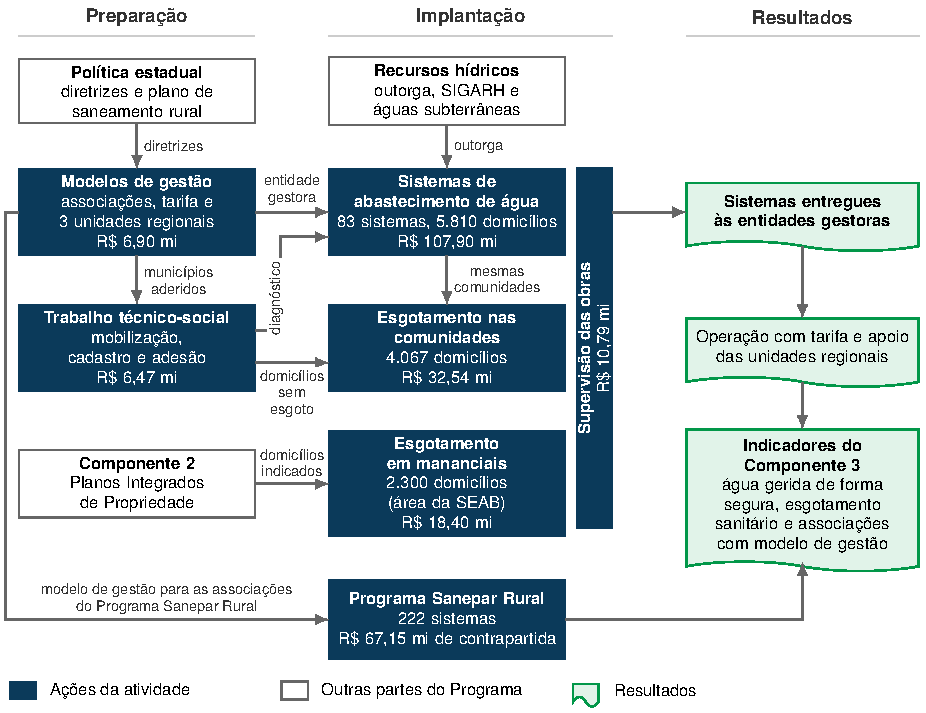
\includegraphics[width=15.68cm]{figuras/f-articulacao.pdf}
  \fonteMOP{Fonte: IAT (2026), com valores da planilha PSH\_CUSTO\_Consolidada (PARANÁ, 2026).}
  % Texto alternativo: Diagrama da articulação entre as sete ações da atividade, da preparação social e institucional à entrega dos sistemas e aos indicadores do componente.
\end{figure}

A Figura~\ref{crono-atividade} apresenta o período de execução e o investimento anual de cada ação.

\begin{figure}[H]
  \centering
  \caption{Período de execução e investimento anual das ações de abastecimento de água e esgotamento sanitário rural (R\$~milhões)}\label{crono-atividade}
  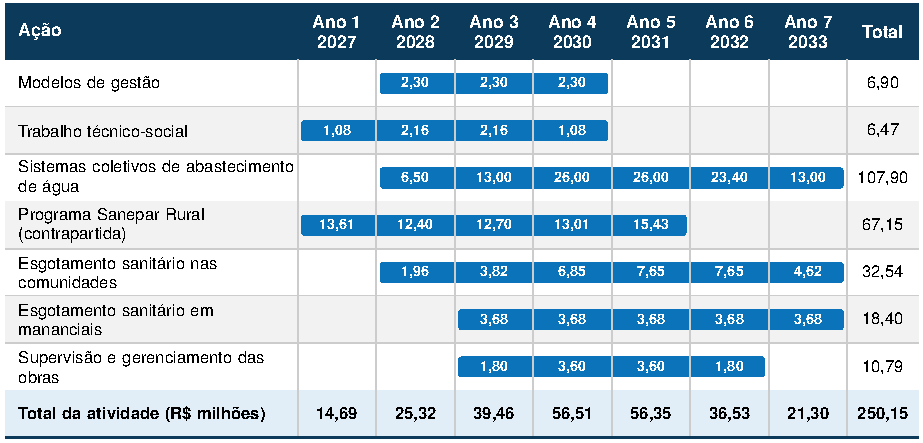
\includegraphics[width=15.64cm]{figuras/g-crono-atividade.pdf}
  \fonteMOP{Fonte: Planilha PSH\_CUSTO\_Consolidada, versão v2408 (PARANÁ, 2026). Valores arredondados; o total anual corresponde à soma dos valores exatos da planilha.}
  % Texto alternativo: Cronograma de 2027 a 2033 com o investimento anual de cada ação e o total da atividade por ano.
\end{figure}

\acao{Ação 3.2.2.1 – Implantação dos modelos de gestão}

\phantomsection
\addcontentsline{toc}{subsection}{1. Contextualização}
\subsection*{1. Contextualização}

A ação estrutura os modelos de gestão responsáveis pela operação e pela manutenção dos sistemas de abastecimento de água e das soluções de esgotamento sanitário implantados na atividade. Os objetivos são: definir, com as prefeituras e as comunidades, o arranjo de gestão de cada sistema; constituir ou regularizar as associações de saneamento rural; instituir a tarifa; e estruturar três unidades regionais de apoio técnico às entidades gestoras (IAT, 2026a; IAT, 2026b).

O Paraná não dispõe de política estadual de saneamento rural que estabeleça modelo de gestão para esses serviços. As iniciativas existentes são descentralizadas, concentram-se no abastecimento de água e são executadas pela Sanepar, por serviços municipais, por arranjos entre o Estado e os municípios e, em parte dos casos, pelas próprias comunidades (IAT, 2026a).

A autogestão comunitária, predominante no meio rural, apresenta deficiências de capacidade técnica, financeira e institucional e carece de apoio do poder público, o que compromete a regularidade e a qualidade da prestação. A dispersão das comunidades e a limitação de pessoal e de recursos dos municípios agravam esse quadro (BRASIL, 2019; IAT, 2026a).

A ação responde pela sustentabilidade dos investimentos da atividade. Sem entidade gestora habilitada a operar o sistema, cobrar a tarifa e executar a manutenção, os poços, as redes e as soluções de esgotamento sanitário tendem à deterioração em poucos anos; por esse motivo, o modelo de gestão é pactuado antes das obras e acompanha cada sistema até a entrega. A contribuição da ação é medida pelo indicador de associações de saneamento rural com modelo de gestão adotado.

\textbf{Inclui:} a definição e o enquadramento jurídico do modelo; a pactuação com os municípios, formalizada em Termo de Cooperação; a constituição ou a regularização das associações e a adesão das famílias; a elaboração de estatutos, manuais e cartilhas; a instituição da tarifa, com tarifa social; a estruturação das três unidades regionais de apoio (equipe técnica, sede, veículo, geração de energia fotovoltaica e custeio de operação e manutenção); e o acompanhamento das entidades gestoras até o encerramento.

\textbf{Não inclui:} as obras dos sistemas de abastecimento de água e das soluções de esgotamento sanitário, o trabalho técnico-social com as famílias e a formulação da política estadual de saneamento rural, objeto de atividade própria do subcomponente.

\textbf{Valor previsto:} R\$~6,90 milhões (empréstimo BIRD: R\$~6,90 milhões; contrapartida: R\$~0,00 milhões), conforme a planilha PSH\_CUSTO\_Consolidada.

\phantomsection
\addcontentsline{toc}{subsection}{2. Área de atuação}
\subsection*{2. Área de atuação}

A ação abrange as comunidades atendidas pelos sistemas coletivos de abastecimento de água do IAT, selecionadas pelos seguintes critérios: 70 ou mais domicílios ocupados; município classificado como de médio baixo ou de médio desempenho no Índice Ipardes de Desempenho Municipal (IPDM); e prioridade para demandas já encaminhadas ao IAT e para associações que já operam sistemas. A seleção preliminar indicou 83 comunidades, com 5.810 domicílios, sendo o número mínimo de domicílios o requisito de viabilidade da gestão (IAT, 2026a). Os modelos de gestão aplicam-se também às associações constituídas no Programa Sanepar Rural.

A Figura~\ref{mapa} apresenta o mapa inicial das áreas potenciais de atuação: 2.571 aglomerados de domicílios rurais situados a menos de 350 m entre si, classificados em nove faixas de número de domicílios, com os limites das associações de municípios e os 112 municípios consorciados ao Consórcio Intermunicipal de Saneamento do Paraná (CISPAR). A presença do consórcio indica as regiões com base institucional para o arranjo intermunicipal, e as maiores concentrações de domicílios (Região Metropolitana de Curitiba, Centro-Sul e Sudeste do Estado) indicam as localizações candidatas às unidades regionais de apoio. A localização das três unidades é definida após a seleção final das comunidades.

\begin{figure}[H]
  \centering
  \caption{Áreas prioritárias, associações de municípios, CISPAR e concentração de domicílios rurais}\label{mapa}
  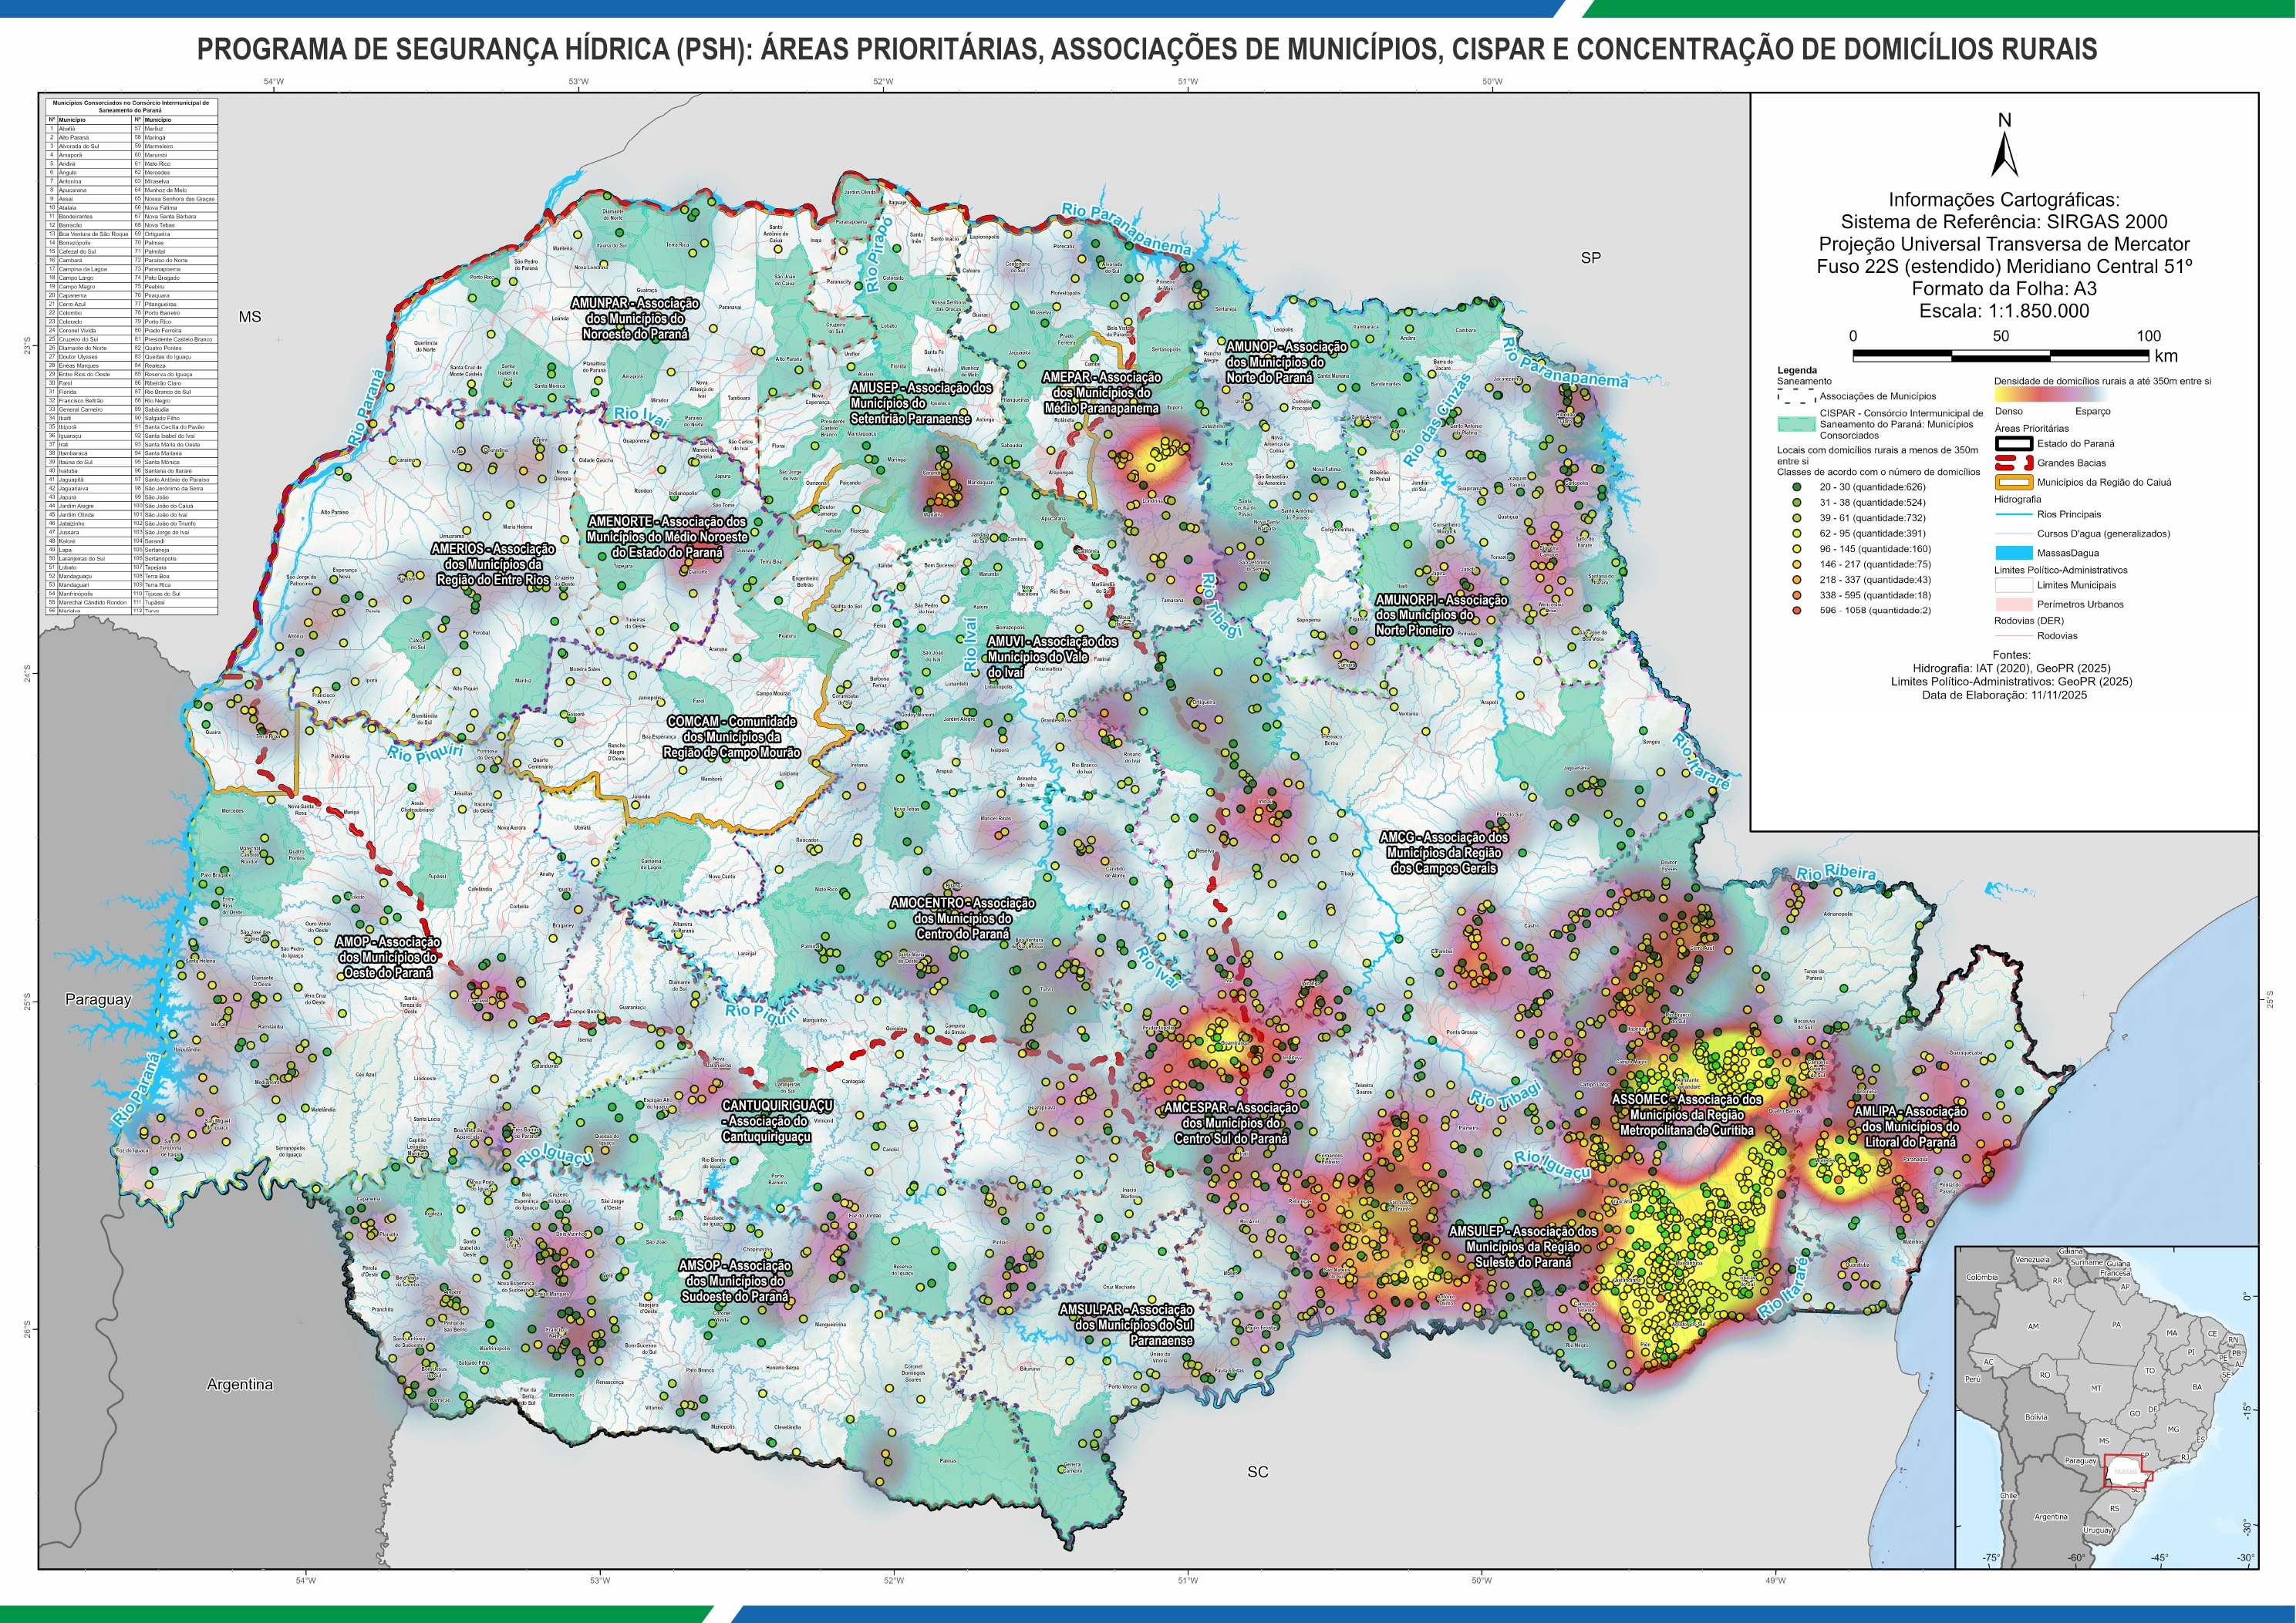
\includegraphics[width=16.00cm]{figuras/f-mapa.jpg}
  \fonteMOP{Fonte: IAT e IDR-Paraná (2025). Hidrografia: IAT (2020) e GeoPR (2025); limites político-administrativos: GeoPR (2025).}
  % Texto alternativo: Mapa do Paraná com as áreas prioritárias do PSH-PR, as associações de municípios, os municípios do CISPAR e os aglomerados de domicílios rurais.
\end{figure}

\pendencia{O Acordo de Empréstimo, item (j)(vii) das definições, exige a identificação das áreas rurais da Parte 3.2 no MOP. O mapa representa o potencial de atuação, e não as 83 comunidades selecionadas; incluir a lista ou o mapa das comunidades e a localização das três unidades regionais.}

\pendencia{Os logos institucionais foram removidos do mapa, conforme o Guia de Identidade Visual (seção 2.6). Na versão final, refazer o mapa sobre a base cartográfica oficial (IAT/ITCG), com as áreas do Programa na cor do Caderno C3 e 40\% de transparência (seção 5.4).}

\phantomsection
\addcontentsline{toc}{subsection}{3. Arranjo institucional e partes interessadas}
\subsection*{3. Arranjo institucional e partes interessadas}

A ação é coordenada pelo IAT, por meio da Diretoria de Saneamento Ambiental e Recursos Hídricos (DISAR), responsável pela definição do modelo, pela pactuação com os municípios e pela constituição e pelo acompanhamento das entidades gestoras. A Secretaria de Estado das Cidades (SECID) valida o modelo de gestão e a tarifa. A UGP acompanha a execução e consolida o reporte ao Banco Mundial.

\pendencia{Indicar a gerência do IAT responsável pela ação (instituição, diretoria e gerência).}

As partes interessadas são:

\begin{itemize}
  \item \textbf{Coexecutores:} a Secretaria de Estado da Agricultura e do Abastecimento (SEAB), na mobilização social e na articulação local, e a Sanepar, nas associações constituídas no Programa Sanepar Rural;
  \item \textbf{Intervenientes:} a SECID, que valida o modelo e a tarifa; as prefeituras, que participam da governança, celebram o Termo de Cooperação, aprovam a lei autorizativa, quando exigida, e apoiam as associações; os consórcios públicos intermunicipais, como o CISPAR, na hipótese de arranjo consorciado; e as empresas contratadas para a equipe técnica e a estrutura das unidades regionais;
  \item \textbf{Comunidades e associações de moradores:} participam da definição do modelo, constituem a entidade gestora e operam os sistemas.
\end{itemize}

Os beneficiários diretos são as associações de saneamento rural e as famílias das comunidades atendidas, que passam a dispor de operação regular, tarifa instituída e suporte técnico. Os beneficiários indiretos são os municípios, que passam a contar com arranjo de gestão para o saneamento rural, e a população das bacias, beneficiada pela manutenção adequada dos sistemas.

\phantomsection
\addcontentsline{toc}{subsection}{4. Processo de execução operacional}
\subsection*{4. Processo de execução operacional}

A ação compreende seis etapas, da definição do modelo ao encerramento dos Termos de Cooperação (Figura~\ref{raias-3221}). Duas premissas orientam a sequência: o modelo de gestão é pactuado antes do início das obras, e nenhum sistema é entregue sem entidade gestora constituída e capacitada para operá-lo.

\begin{figure}[H]
  \centering
  \caption{Fluxograma da implantação dos modelos de gestão: entradas, etapas por responsável e saídas}\label{raias-3221}
  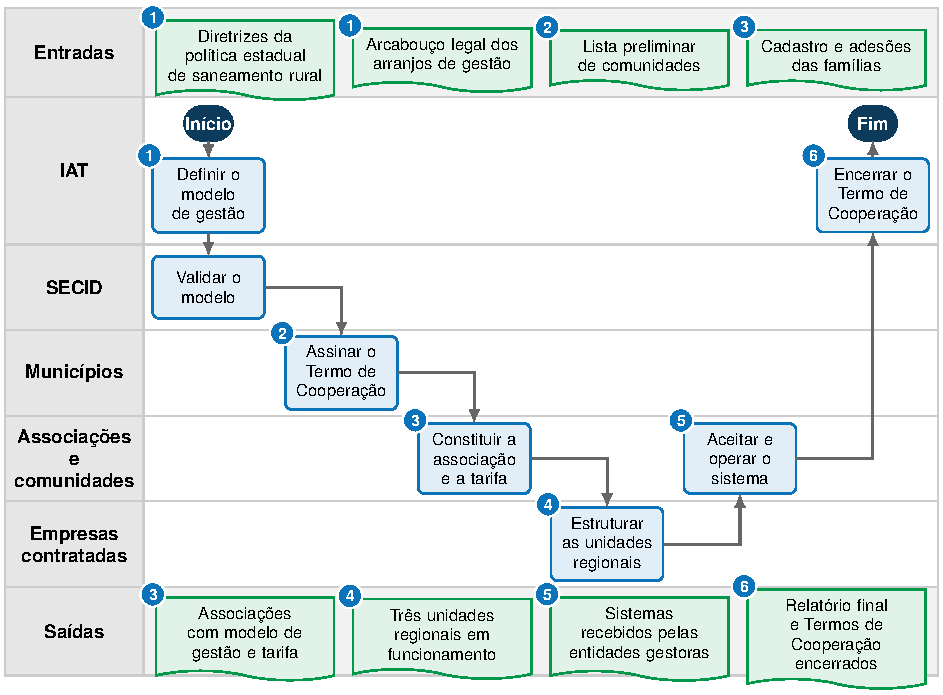
\includegraphics[width=15.96cm]{figuras/g-raias-3221.pdf}
  \fonteMOP{Fonte: IAT (2026).}
  % Texto alternativo: Fluxograma em raias da implantação dos modelos de gestão, com uma raia por instituição, as etapas numeradas na raia do executor, as entradas no topo e as saídas na base.
\end{figure}

\phantomsection
\subsubsection*{4.1 Etapa 1: Estudos preliminares e definição do modelo}

\textbf{Atividades:} seleção dos instrumentos de gestão; definição dos parceiros, dos critérios e dos indicadores; enquadramento jurídico da proposta; e definição da estratégia de comunicação do modelo. Estão em análise três alternativas de arranjo (Quadro~\ref{alternativas}).

Na primeira alternativa, a associação de moradores opera o sistema da respectiva localidade. Na condição de organização da sociedade civil, a associação submete-se ao Marco Regulatório das Organizações da Sociedade Civil (MROSC), e o uso da infraestrutura pública é formalizado por Acordo de Cooperação, após a aprovação de lei municipal autorizativa (BRASIL, 2014).

Na segunda, as associações filiam-se a uma central que lhes presta apoio técnico, administrativo e financeiro. Trata-se do modelo do Sistema Integrado de Saneamento Rural (SISAR) do Ceará, que, em agosto de 2025, atendia mais de 1,13 milhão de pessoas, cerca de 56\% da população rural do estado, em 174 municípios e 1.466 localidades (CEARÁ, 2025). As Centrais de Associações Comunitárias da Bahia adotam arranjo equivalente e executaram 16.888 novas ligações de água e a recuperação de outras 5.297, em 49 municípios (BAHIA, 2022).

\begin{quadro}[H]
  \caption{Alternativas de modelo de gestão e respectivo amparo legal}\label{alternativas}
  \footnotesize\renewcommand{\arraystretch}{1.25}\setlength{\tabcolsep}{5pt}
  \begin{tabular}{>{\raggedright\arraybackslash}p{\dimexpr 0.1874\linewidth-2\tabcolsep\relax}>{\raggedright\arraybackslash}p{\dimexpr 0.2709\linewidth-2\tabcolsep\relax}>{\raggedright\arraybackslash}p{\dimexpr 0.2709\linewidth-2\tabcolsep\relax}>{\raggedright\arraybackslash}p{\dimexpr 0.2709\linewidth-2\tabcolsep\relax}}
    \rowcolor{azulEscuro}\textcolor{white}{\textbf{Aspecto}} & \textcolor{white}{\textbf{Associação de moradores}} & \textcolor{white}{\textbf{Central de associações}} & \textcolor{white}{\textbf{Consórcio público}} \\
    \textbf{Funcionamento} & Moradores organizados operam o sistema da localidade, com apoio da prefeitura & Associações filiadas a uma central, que presta apoio técnico, administrativo e financeiro & Municípios consorciados prestam o serviço de forma associada \\ \arrayrulecolor{cinza20}\hline
    \rowcolor{cinza5}\textbf{Amparo legal} & MROSC (Lei nº~13.019/2014) & MROSC; a nota técnica cita também o Decreto nº~11.599/2023 e a Portaria nº~2.777/2025 da Fundação Nacional de Saúde (Funasa) & Lei dos Consórcios Públicos (Lei nº~11.107/2005) e Lei nº~11.445/2007 \\ \arrayrulecolor{cinza20}\hline
    \textbf{Instrumento} & Acordo de Cooperação, após lei municipal que autoriza a cessão dos ativos & Acordo de Cooperação com o poder público, após lei municipal autorizativa & Alteração do contrato de consórcio; contrato de rateio; cessão de uso dos ativos \\ \arrayrulecolor{cinza20}\hline
    \rowcolor{cinza5}\textbf{Referência} & Associações de moradores que já operam sistemas no Paraná & SISAR (CE): 1,13 milhão de pessoas em 1.466 localidades; Centrais de Associações (BA) & CISPAR: 112 municípios consorciados no Paraná \\ \noalign{\global\arrayrulewidth=1pt}\arrayrulecolor{azulEscuro}\hline\noalign{\global\arrayrulewidth=0.4pt}
  \end{tabular}
  \fonteMOP{Fonte: IAT (2026), com base em IAT (2026a), CEARÁ (2025) e BAHIA (2022).}
  \notaMOP{Nota: em todas as alternativas, o modelo é definido com a prefeitura e a comunidade, mediante abordagem participativa, com tarifa social e capacitação dos operadores.}
\end{quadro}

Na terceira, os municípios prestam o serviço de forma associada, por meio de consórcio público (BRASIL, 2005). Esta é a alternativa preliminarmente indicada para o Paraná, em razão da participação de grande parte dos municípios em consórcios, a exemplo dos 112 municípios consorciados ao CISPAR. O objeto do consórcio existente pode ser ampliado para o abastecimento de água e o esgotamento sanitário rurais, mediante alteração contratual aprovada em assembleia e ratificada por lei de cada ente.

O contrato de rateio define a contribuição anual de cada município, e os poços, as redes e os reservatórios podem ser cedidos ao consórcio, com reversão ao município ao término do contrato. O arranjo proporciona ganho de escala, compartilha a estrutura técnica e administrativa e confere continuidade à gestão entre mandatos. A nota técnica do componente cita, ainda, o Decreto nº~11.599/2023 e a Portaria Funasa nº~2.777/2025 como fundamento dos arranjos associativos no marco legal do saneamento atualizado pela Lei nº~14.026/2020 (IAT, 2026a).

\pendencia{Conferir o fundamento legal citado pela nota técnica. O Decreto nº~11.599/2023 trata da prestação regionalizada e do apoio técnico e financeiro da União; a Portaria Funasa nº~2.777/2025 consta no portal da Funasa como seleção de propostas de abastecimento de água, esgotamento sanitário e melhorias sanitárias domiciliares em áreas rurais, e não como diretriz de modelo de gestão. Ver a planilha de referências normativas.}

\pendencia{A nota técnica prevê contrato de programa no arranjo consorciado. A Lei nº~14.026/2020 alterou a Lei nº~11.445/2007 e restringiu esse instrumento na prestação de serviços de saneamento; confirmar com a assessoria jurídica o instrumento adequado à prestação pelo consórcio.}

\textbf{Entradas:} diretrizes da política estadual de saneamento rural, quando disponíveis; experiências de referência; legislação aplicável.

\textbf{Responsáveis:} IAT (executa), com consulta à SEAB e às prefeituras; SECID (valida o modelo).

\textbf{Produto:} modelo de gestão definido, com enquadramento jurídico.

\pendencia{O modelo de gestão encontra-se em definição. Registrar neste item a alternativa adotada e o parecer jurídico, após a aprovação.}

\phantomsection
\subsubsection*{4.2 Etapa 2: Pactuação com municípios e comunidades}

\textbf{Atividades:} a pactuação inicia-se pelo município e estende-se à comunidade (Figura~\ref{adesao}). O IAT define os critérios, seleciona as comunidades e sensibiliza as prefeituras; o município formaliza a adesão e celebra com o IAT o Termo de Cooperação, que estabelece as obrigações das partes até a entrega dos sistemas. Quando o arranjo envolve cessão de bens públicos, o município aprova a lei autorizativa; em seguida, o IAT contata a comunidade, que manifesta o interesse por meio de contrato de pré-adesão.

\begin{figure}[H]
  \centering
  \caption{Seleção e adesão dos municípios e das comunidades, por responsável}\label{adesao}
  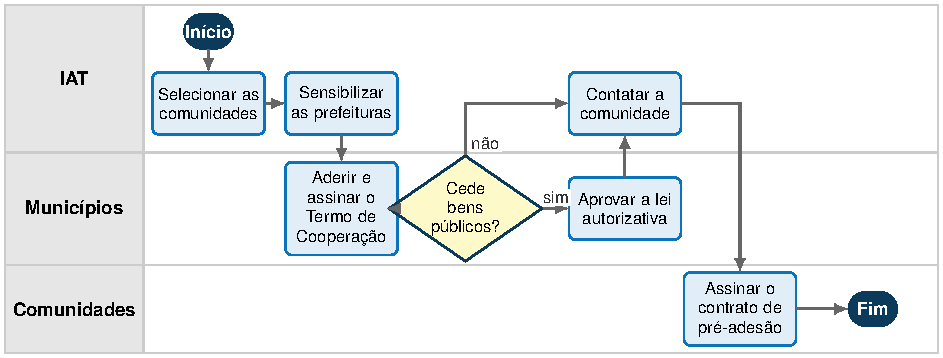
\includegraphics[width=15.96cm]{figuras/f-adesao.pdf}
  \fonteMOP{Fonte: IAT (2026), com base em IAT (2026b).}
  % Texto alternativo: Fluxograma em raias do IAT, dos municípios e das comunidades, da seleção das comunidades à pré-adesão, com a decisão sobre a lei autorizativa.
\end{figure}

\textbf{Entradas:} modelo de gestão definido (Etapa 1); lista preliminar de comunidades; minuta do Termo de Cooperação.

\textbf{Responsáveis:} IAT e prefeituras (executam); SEAB e comunidades (consultadas); IAT (aprova os termos).

\textbf{Produto:} Termos de Cooperação assinados e contratos de pré-adesão.

\phantomsection
\subsubsection*{4.3 Etapa 3: Constituição das entidades gestoras}

\textbf{Atividades:} após a adesão da comunidade, o IAT apoia a constituição ou a regularização da associação de saneamento rural: elabora o estatuto, os manuais e as cartilhas, formaliza a adesão de cada família e acompanha o registro da associação. A tarifa é aprovada em assembleia, com tarifa social para as famílias de baixa renda, e validada pela SECID. A etapa utiliza o cadastro e os termos de adesão do trabalho técnico-social e é concluída antes do início da obra de cada sistema.

\textbf{Entradas:} contratos de pré-adesão; cadastro e termos de adesão das famílias (trabalho técnico-social).

\textbf{Responsáveis:} IAT e associações (executam); prefeituras (consultadas); SECID (valida a tarifa).

\textbf{Produto:} associação regularizada, com tarifa instituída.

\phantomsection
\subsubsection*{4.4 Etapa 4: Estruturação das unidades regionais de apoio}

\textbf{Atividades:} cada uma das três unidades previstas na planilha de custos constitui estrutura regional de apoio às associações, com equipe técnica, sede, veículo, geração de energia fotovoltaica e custeio de operação e manutenção (IAT, 2026a). As unidades elaboram os manuais de desempenho operacional, estruturam o monitoramento e capacitam os dirigentes e os operadores das associações. Implanta-se uma unidade por ano, de 2028 a 2030, conforme a entrada em operação dos primeiros sistemas.

\textbf{Entradas:} modelo e localização das unidades definidos; associações constituídas.

\textbf{Responsáveis:} IAT (executa e aprova) e empresas contratadas (executam); associações (informadas).

\textbf{Produto:} unidade regional em funcionamento e pessoal capacitado.

\pendencia{A nota técnica do componente estima as três unidades em R\$~6,63 milhões, e a planilha de custos, em R\$~6,90 milhões; prevalece a planilha. Confirmar a composição de cada unidade e a fonte de custeio da operação após 2030.}

\phantomsection
\subsubsection*{4.5 Etapa 5: Entrega dos sistemas e acompanhamento}

\textbf{Atividades:} concluída a obra, a entrega é formalizada em reunião técnica com a comunidade e a entidade gestora, que atesta o recebimento por termo de aceite. A partir da entrega, a entidade gestora opera e mantém o sistema com suporte da unidade regional, e o IAT avalia o desempenho semestralmente, com base nos dados registrados no Sistema de Gestão Ambiental e de Recursos Hídricos (SIGARH) e na plataforma GeoPR. As entregas acompanham o cronograma de implantação dos sistemas de abastecimento.

\textbf{Entradas:} sistemas de abastecimento de água e soluções de esgotamento sanitário concluídos; associação regularizada.

\textbf{Responsáveis:} IAT e entidade gestora (executam); entidade gestora (aceita o sistema); prefeituras (consultadas).

\textbf{Produto:} termos de aceite assinados e relatórios semestrais de desempenho.

\phantomsection
\subsubsection*{4.6 Etapa 6: Encerramento}

\textbf{Atividades:} consolidação dos resultados, relatório final, prestação de contas e encerramento do Termo de Cooperação com cada município.

\textbf{Entradas:} relatórios semestrais; Termos de Recebimento Definitivo dos sistemas.

\textbf{Responsáveis:} IAT (executa); UGP (valida).

\textbf{Produto:} relatório final e Termos de Cooperação encerrados.

\phantomsection
\subsubsection*{4.7 Modalidade de execução}

O item de custo é a implantação do modelo de gestão: três unidades de R\$~2,3 milhões, no total de R\$~6,90 milhões, com recursos do empréstimo do BIRD. Na planilha, o produto consta como “Sistema coletivo de abastecimento de água e individual de tratamento de efluentes”.

As Etapas 1, 2, 3, 5 e 6 são executadas diretamente pela equipe do IAT, com Termo de Cooperação com cada município. A Etapa 4 é executada mediante licitação, conforme o Caderno AQ: serviços de consultoria para a equipe técnica das unidades, aquisição de bens (veículos e sistemas fotovoltaicos) e serviços de adequação das sedes.

\pendencia{Confirmar no Plano de Aquisições a divisão dos processos da Etapa 4 (consultoria, bens e serviços).}

\pendencia{Completar as remissões aos cadernos transversais com a seção correspondente (por exemplo, “Caderno AQ, seção 4”), conforme o Guia de Identidade Visual (seção 2.5), quando a numeração desses cadernos estiver definida.}

\phantomsection
\addcontentsline{toc}{subsection}{5. Matriz de responsabilidades}
\subsection*{5. Matriz de responsabilidades}

O Quadro~\ref{raci-3221} apresenta o papel de cada parte em cada etapa.

\begin{quadro}[H]
  \caption{Matriz de responsabilidades da implantação dos modelos de gestão}\label{raci-3221}
  \footnotesize\renewcommand{\arraystretch}{1.25}\setlength{\tabcolsep}{3pt}
  \begin{tabular}{>{\raggedright\arraybackslash}p{\dimexpr 0.2536\linewidth-2\tabcolsep\relax}>{\centering\arraybackslash}p{\dimexpr 0.0882\linewidth-2\tabcolsep\relax}>{\centering\arraybackslash}p{\dimexpr 0.0882\linewidth-2\tabcolsep\relax}>{\centering\arraybackslash}p{\dimexpr 0.0882\linewidth-2\tabcolsep\relax}>{\centering\arraybackslash}p{\dimexpr 0.0882\linewidth-2\tabcolsep\relax}>{\centering\arraybackslash}p{\dimexpr 0.0882\linewidth-2\tabcolsep\relax}>{\centering\arraybackslash}p{\dimexpr 0.0882\linewidth-2\tabcolsep\relax}>{\centering\arraybackslash}p{\dimexpr 0.2173\linewidth-2\tabcolsep\relax}}
    \rowcolor{azulEscuro}\textcolor{white}{\textbf{Parte}} & \textcolor{white}{\textbf{E1}} & \textcolor{white}{\textbf{E2}} & \textcolor{white}{\textbf{E3}} & \textcolor{white}{\textbf{E4}} & \textcolor{white}{\textbf{E5}} & \textcolor{white}{\textbf{E6}} & \textcolor{white}{\textbf{Produto final}} \\
    IAT & \raci{R} & \raci{R} \raci{A} & \raci{R} & \raci{R} \raci{A} & \raci{R} & \raci{R} & \raci{R} \\ \arrayrulecolor{cinza20}\hline
    \rowcolor{cinza5}SECID & \raci{A} & \raci{I} & \raci{A} & \raci{I} & \raci{I} & \raci{I} & \raci{A} \\ \arrayrulecolor{cinza20}\hline
    SEAB & \raci{C} & \raci{C} & – & – & \raci{I} & \raci{I} & \raci{I} \\ \arrayrulecolor{cinza20}\hline
    \rowcolor{cinza5}Prefeituras & \raci{C} & \raci{R} & \raci{C} & \raci{I} & \raci{C} & \raci{C} & \raci{I} \\ \arrayrulecolor{cinza20}\hline
    Associações e comunidades & – & \raci{C} & \raci{R} & \raci{I} & \raci{A} & \raci{I} & \raci{R} \\ \arrayrulecolor{cinza20}\hline
    \rowcolor{cinza5}Empresas contratadas & – & – & – & \raci{R} & – & – & – \\ \arrayrulecolor{cinza20}\hline
    UGP & \raci{I} & \raci{I} & \raci{I} & \raci{I} & \raci{I} & \raci{A} & \raci{I} \\ \noalign{\global\arrayrulewidth=1pt}\arrayrulecolor{azulEscuro}\hline\noalign{\global\arrayrulewidth=0.4pt}
  \end{tabular}
  \fonteMOP{Fonte: IAT (2026).}
  \notaMOP{Nota: E1 a E6 correspondem às Etapas 1 a 6 do item 4. \raci{R} executa (pode haver mais de um); \raci{A} aprova ou valida o produto (um por etapa); \raci{C} é consultado previamente; \raci{I} é informado posteriormente. Produto final: associações de saneamento rural com modelo de gestão adotado.}
\end{quadro}

\phantomsection
\addcontentsline{toc}{subsection}{6. Metas, indicadores e comprovação}
\subsection*{6. Metas, indicadores e comprovação}

A meta física da ação é a implantação de três unidades regionais de apoio, uma por ano, de 2028 a 2030 (Quadro~\ref{metas-3221}). As entidades gestoras são constituídas à medida que os sistemas são concluídos.

\begin{quadro}[H]
  \caption{Metas anuais da implantação dos modelos de gestão}\label{metas-3221}
  \footnotesize\renewcommand{\arraystretch}{1.25}\setlength{\tabcolsep}{3pt}
  \begin{tabular}{>{\raggedright\arraybackslash}p{\dimexpr 0.2095\linewidth-2\tabcolsep\relax}>{\raggedright\arraybackslash}p{\dimexpr 0.1268\linewidth-2\tabcolsep\relax}>{\raggedleft\arraybackslash}p{\dimexpr 0.0794\linewidth-2\tabcolsep\relax}>{\raggedleft\arraybackslash}p{\dimexpr 0.0794\linewidth-2\tabcolsep\relax}>{\raggedleft\arraybackslash}p{\dimexpr 0.0794\linewidth-2\tabcolsep\relax}>{\raggedleft\arraybackslash}p{\dimexpr 0.0794\linewidth-2\tabcolsep\relax}>{\raggedleft\arraybackslash}p{\dimexpr 0.0794\linewidth-2\tabcolsep\relax}>{\raggedleft\arraybackslash}p{\dimexpr 0.0794\linewidth-2\tabcolsep\relax}>{\raggedleft\arraybackslash}p{\dimexpr 0.0794\linewidth-2\tabcolsep\relax}>{\raggedleft\arraybackslash}p{\dimexpr 0.1081\linewidth-2\tabcolsep\relax}}
    \rowcolor{azulEscuro}\textcolor{white}{\textbf{Produto}} & \textcolor{white}{\textbf{Unidade}} & \centering\arraybackslash \textcolor{white}{\textbf{Ano 1}} & \centering\arraybackslash \textcolor{white}{\textbf{Ano 2}} & \centering\arraybackslash \textcolor{white}{\textbf{Ano 3}} & \centering\arraybackslash \textcolor{white}{\textbf{Ano 4}} & \centering\arraybackslash \textcolor{white}{\textbf{Ano 5}} & \centering\arraybackslash \textcolor{white}{\textbf{Ano 6}} & \centering\arraybackslash \textcolor{white}{\textbf{Ano 7}} & \centering\arraybackslash \textcolor{white}{\textbf{Total}} \\
    Unidades regionais do modelo de gestão implantadas & unidades & – & 1 & 1 & 1 & – & – & – & 3 \\ \noalign{\global\arrayrulewidth=1pt}\arrayrulecolor{azulEscuro}\hline\noalign{\global\arrayrulewidth=0.4pt}
  \end{tabular}
  \fonteMOP{Fonte: Planilha PSH\_CUSTO\_Consolidada, versão v2408 (PARANÁ, 2026).}
  \notaMOP{Nota: Ano 1 = 2027 e Ano 7 = 2033. Na planilha, o produto consta como “Sistema coletivo de abastecimento de água e individual de tratamento de efluentes”.}
\end{quadro}

O Quadro~\ref{ind-3221} reúne os indicadores de andamento e de resultado da ação. O principal é o indicador de associações de saneamento rural com modelo de gestão adotado, medido pelo número acumulado de associações que formalizaram a adoção do modelo.

\begin{quadro}[H]
  \caption{Indicadores da implantação dos modelos de gestão}\label{ind-3221}
  \footnotesize\renewcommand{\arraystretch}{1.25}\setlength{\tabcolsep}{3pt}
  \begin{tabular}{>{\raggedright\arraybackslash}p{\dimexpr 0.3165\linewidth-2\tabcolsep\relax}>{\raggedright\arraybackslash}p{\dimexpr 0.1378\linewidth-2\tabcolsep\relax}>{\raggedleft\arraybackslash}p{\dimexpr 0.1102\linewidth-2\tabcolsep\relax}>{\raggedleft\arraybackslash}p{\dimexpr 0.1599\linewidth-2\tabcolsep\relax}>{\raggedright\arraybackslash}p{\dimexpr 0.2756\linewidth-2\tabcolsep\relax}}
    \rowcolor{azulEscuro}\textcolor{white}{\textbf{Indicador}} & \textcolor{white}{\textbf{Unidade}} & \centering\arraybackslash \textcolor{white}{\textbf{Linha de base (2025)}} & \centering\arraybackslash \textcolor{white}{\textbf{Meta}} & \textcolor{white}{\textbf{Frequência e fonte dos dados}} \\
    Associações de saneamento rural com modelo de gestão adotado (indicador do componente) & associações (acumulado) & 0 & 122 & Anual; IAT, Sanepar e cadastro das associações \\ \arrayrulecolor{cinza20}\hline
    \rowcolor{cinza5}Unidades regionais de apoio em funcionamento & unidades & 0 & 3 & Anual; IAT \\ \arrayrulecolor{cinza20}\hline
    Sistemas recebidos pela entidade gestora com termo de aceite & sistemas & 0 & 83 & Semestral; IAT \\ \arrayrulecolor{cinza20}\hline
    \rowcolor{cinza5}Domicílios atendidos com tarifa instituída & domicílios & 0 & 5.810 & Anual; associações e IAT \\ \noalign{\global\arrayrulewidth=1pt}\arrayrulecolor{azulEscuro}\hline\noalign{\global\arrayrulewidth=0.4pt}
  \end{tabular}
  \fonteMOP{Fonte: IAT (2026).}
\end{quadro}

\pendencia{O MOP de março previa 122 associações até 2032, no período de 2027 a 2032. Atualizar as metas anuais para o período de 2027 a 2033 e explicitar a composição do total (comunidades atendidas pelo IAT e associações do Programa Sanepar Rural).}

Os critérios de aceite e as evidências de comprovação de cada produto constam do Quadro~\ref{aceite-3221}. A sustentabilidade do resultado é verificada após a entrega: a entidade gestora deve estar em operação, com tarifa cobrada, associação ativa e relatório semestral de desempenho.

\begin{quadro}[H]
  \caption{Critérios de aceite e evidências da implantação dos modelos de gestão}\label{aceite-3221}
  \footnotesize\renewcommand{\arraystretch}{1.25}\setlength{\tabcolsep}{5pt}
  \begin{tabular}{>{\raggedright\arraybackslash}p{\dimexpr 0.2150\linewidth-2\tabcolsep\relax}>{\raggedright\arraybackslash}p{\dimexpr 0.3386\linewidth-2\tabcolsep\relax}>{\raggedright\arraybackslash}p{\dimexpr 0.2921\linewidth-2\tabcolsep\relax}>{\raggedright\arraybackslash}p{\dimexpr 0.1543\linewidth-2\tabcolsep\relax}}
    \rowcolor{azulEscuro}\textcolor{white}{\textbf{Produto}} & \textcolor{white}{\textbf{Critério de aceite}} & \textcolor{white}{\textbf{Evidência de comprovação}} & \textcolor{white}{\textbf{Responsável pela validação}} \\
    Modelo de gestão definido & Arranjo definido para cada conjunto de comunidades, com enquadramento jurídico & Nota técnica do modelo e parecer jurídico & SECID \\ \arrayrulecolor{cinza20}\hline
    \rowcolor{cinza5}Termo de Cooperação & Assinado pelo município, com obrigações, prazos e contrapartidas & Termo assinado e publicado & IAT \\ \arrayrulecolor{cinza20}\hline
    Contratos de pré-adesão & Assinados pelas famílias interessadas da comunidade & Contratos assinados; número de associados & IAT \\ \arrayrulecolor{cinza20}\hline
    \rowcolor{cinza5}Associação regularizada & Estatuto registrado e inscrição ativa no Cadastro Nacional da Pessoa Jurídica (CNPJ) & Registro em cartório; comprovante de inscrição no CNPJ & IAT \\ \arrayrulecolor{cinza20}\hline
    Tarifa instituída & Aprovada em assembleia, com tarifa social para famílias de baixa renda & Ata da assembleia; regulamento tarifário & SECID \\ \arrayrulecolor{cinza20}\hline
    \rowcolor{cinza5}Unidade regional em funcionamento & Equipe contratada, sede e veículo em operação & Contratos; termo de recebimento dos bens; relatório de atividades & IAT \\ \arrayrulecolor{cinza20}\hline
    Pessoal capacitado & Conteúdo e carga horária do plano de capacitação cumpridos & Listas de presença e certificados & IAT \\ \arrayrulecolor{cinza20}\hline
    \rowcolor{cinza5}Sistema aceito pela entidade gestora & Sistema recebido sem pendências & Termo de aceite assinado & IAT \\ \arrayrulecolor{cinza20}\hline
    Desempenho acompanhado & Relatório semestral entregue e aprovado & Relatório com dados registrados no SIGARH e no GeoPR & UGP \\ \noalign{\global\arrayrulewidth=1pt}\arrayrulecolor{azulEscuro}\hline\noalign{\global\arrayrulewidth=0.4pt}
  \end{tabular}
  \fonteMOP{Fonte: IAT (2026).}
\end{quadro}

\phantomsection
\addcontentsline{toc}{subsection}{7. Gestão de riscos e impactos ambientais e sociais}
\subsection*{7. Gestão de riscos e impactos ambientais e sociais}

A ação tem natureza institucional e social, e as intervenções físicas restringem-se à adequação das sedes das unidades regionais, de pequeno porte. Os riscos concentram-se na exclusão de famílias vulneráveis ou de comunidades tradicionais, nos conflitos pelo uso da água e na sustentabilidade financeira das associações. O Quadro~\ref{nas-3221} indica as NAS aplicáveis e as respectivas medidas.

As NAS 3, 5, 6 e 8 não se aplicam de forma específica à ação, e a NAS 9 não se aplica ao Programa. Os instrumentos de gestão ambiental e social (Marco de Gestão Ambiental e Social – MGAS, Plano de Engajamento das Partes Interessadas – PEPI e Mecanismo de Queixas e Reclamações – MQR) constam do Caderno AS.

\begin{quadro}[H]
  \caption{Aplicação das Normas Ambientais e Sociais à implantação dos modelos de gestão}\label{nas-3221}
  \footnotesize\renewcommand{\arraystretch}{1.25}\setlength{\tabcolsep}{5pt}
  \begin{tabular}{>{\raggedright\arraybackslash}p{\dimexpr 0.1874\linewidth-2\tabcolsep\relax}>{\raggedright\arraybackslash}p{\dimexpr 0.3716\linewidth-2\tabcolsep\relax}>{\raggedright\arraybackslash}p{\dimexpr 0.4410\linewidth-2\tabcolsep\relax}}
    \rowcolor{azulEscuro}\textcolor{white}{\textbf{NAS}} & \textcolor{white}{\textbf{Aplicação à ação}} & \textcolor{white}{\textbf{Medidas e instrumentos}} \\
    NAS 1 – Avaliação e gestão de riscos & Riscos sociais do modelo: exclusão de famílias, conflitos pelo uso da água e inadimplência & Triagem socioambiental das comunidades; tarifa social; avaliação semestral de desempenho (MGAS) \\ \arrayrulecolor{cinza20}\hline
    \rowcolor{cinza5}NAS 2 – Condições de trabalho & Trabalhadores das empresas que compõem as equipes das unidades regionais & Cláusulas trabalhistas nos contratos; Procedimentos de Gestão de Mão de Obra \\ \arrayrulecolor{cinza20}\hline
    NAS 7 – Povos indígenas e comunidades tradicionais & Comunidades tradicionais ou indígenas nas áreas selecionadas & Identificação na seleção; consulta culturalmente adequada; arranjo compatível com a organização da comunidade (MGAS e PEPI) \\ \arrayrulecolor{cinza20}\hline
    \rowcolor{cinza5}NAS 10 – Engajamento das partes interessadas & Participação das prefeituras e das comunidades na definição do modelo e da tarifa & Reuniões com linguagem acessível; consulta às comunidades; divulgação do Mecanismo de Queixas e Reclamações (PEPI e MQR) \\ \noalign{\global\arrayrulewidth=1pt}\arrayrulecolor{azulEscuro}\hline\noalign{\global\arrayrulewidth=0.4pt}
  \end{tabular}
  \fonteMOP{Fonte: IAT (2026), com base nos instrumentos do Caderno AS.}
\end{quadro}

\phantomsection
\addcontentsline{toc}{subsection}{8. Cronograma}
\subsection*{8. Cronograma}

As etapas acompanham a implantação dos sistemas (Figura~\ref{crono-3221}). A definição do modelo ocorre em 2027; a pactuação, de 2027 a 2030; a constituição das entidades gestoras, de 2028 a 2032, sempre antes da obra de cada sistema; e a estruturação das unidades regionais, uma por ano, de 2028 a 2030. As entregas seguem o cronograma de implantação dos sistemas de abastecimento (5 sistemas em 2028, 10 em 2029, 20 em 2030 e em 2031, 18 em 2032 e 10 em 2033), e a ação é encerrada em 2033.

\begin{figure}[H]
  \centering
  \caption{Cronograma das etapas e das entregas da implantação dos modelos de gestão}\label{crono-3221}
  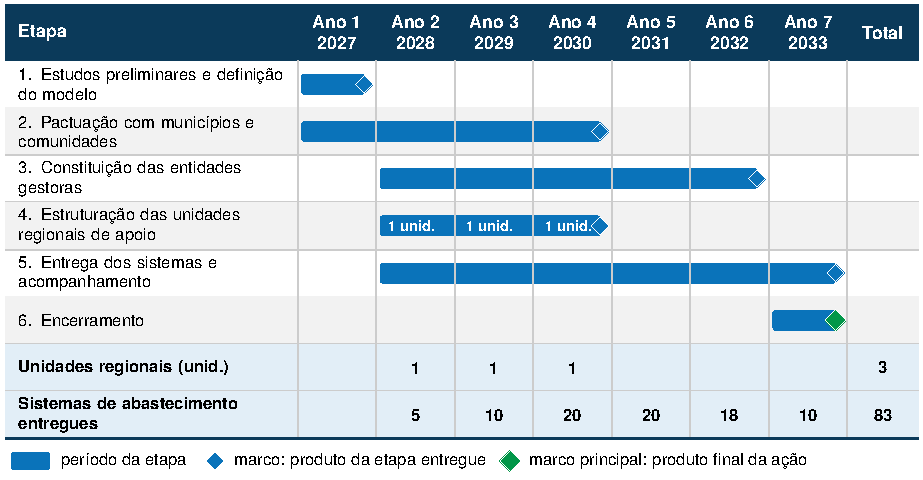
\includegraphics[width=15.64cm]{figuras/g-crono-3221.pdf}
  \fonteMOP{Fonte: IAT (2026), com quantidades da planilha PSH\_CUSTO\_Consolidada (PARANÁ, 2026).}
  % Texto alternativo: Cronograma anual de 2027 a 2033 com as etapas e as quantidades a entregar da implantação dos modelos de gestão.
\end{figure}

\phantomsection
\addcontentsline{toc}{subsection}{9. Interfaces e dependências}
\subsection*{9. Interfaces e dependências}

A ação depende das diretrizes da política estadual de saneamento rural, do cadastro e das adesões do trabalho técnico-social e da conclusão dos sistemas de abastecimento de água e das soluções de esgotamento sanitário. Em contrapartida, fornece às demais ações os municípios aderidos e a entidade gestora definida antes de cada obra, aplica o modelo às associações do Programa Sanepar Rural e alimenta o indicador de associações reportado à UGP (Figura~\ref{interf-3221}).

\begin{figure}[H]
  \centering
  \caption{Interfaces e dependências da implantação dos modelos de gestão}\label{interf-3221}
  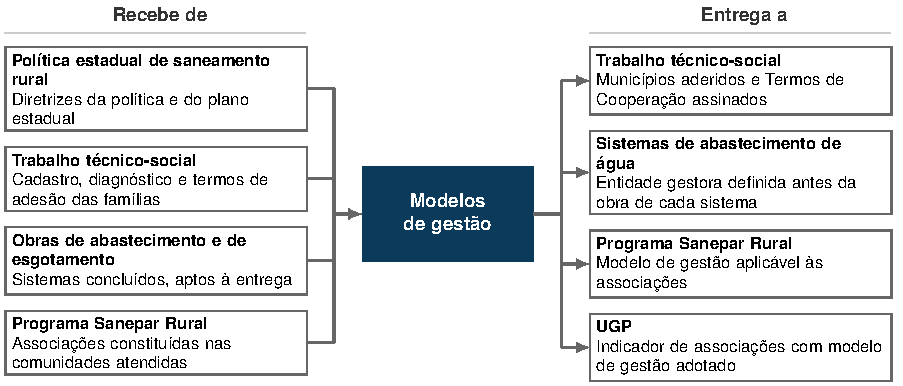
\includegraphics[width=15.30cm]{figuras/g-interf-3221.pdf}
  \fonteMOP{Fonte: IAT (2026).}
  % Texto alternativo: Diagrama das interfaces da implantação dos modelos de gestão: insumos recebidos de outras partes do Programa e produtos entregues a elas.
\end{figure}

\phantomsection
\addcontentsline{toc}{subsection}{10. Documentos complementares}
\subsection*{10. Documentos complementares}

\begin{itemize}
  \item Termo de Cooperação entre o IAT e cada município (minuta a elaborar);
  \item Modelos de estatuto, manuais de desempenho operacional e cartilhas das associações (a elaborar);
  \item Termo de Referência da equipe técnica das unidades regionais (a elaborar);
  \item Lei nº~13.019/2014 (MROSC), Lei nº~11.107/2005 (consórcios públicos), Lei nº~11.445/2007, com a redação da Lei nº~14.026/2020 (marco legal do saneamento), e Decreto nº~11.599/2023;
  \item Programa Nacional de Saneamento Rural (BRASIL, 2019);
  \item Caderno AS (MGAS, PEPI e Mecanismo de Queixas e Reclamações) e Caderno AQ;
  \item Notas técnicas de origem (IAT, 2026a; IAT, 2026b).
\end{itemize}

\acao{Ação 3.2.2.2 – Trabalho técnico-social}

\phantomsection
\addcontentsline{toc}{subsection}{1. Contextualização}
\subsection*{1. Contextualização}

O trabalho técnico-social caracteriza as famílias e as condições de saneamento de cada comunidade, define o público a ser atendido e valida socialmente as soluções técnicas. Compreende também a mobilização da população, a educação sanitária e ambiental, a capacitação das lideranças locais e o estímulo à gestão participativa dos serviços, de modo que cada comunidade disponha de grupo organizado para a gestão dos sistemas (IAT, 2026a; IAT, 2026b).

A ausência de participação das famílias está associada à subutilização e ao abandono de sistemas de saneamento rural. O Programa Nacional de Saneamento Rural estabelece a educação e a participação social como um dos três eixos indissociáveis do saneamento rural, ao lado da gestão dos serviços e da tecnologia (BRASIL, 2019). Há, ainda, o risco de exclusão de famílias vulneráveis, de áreas remotas ou de comunidades tradicionais quando o levantamento se apoia apenas em cadastros preexistentes.

A ação produz as informações das quais dependem as demais. O diagnóstico subsidia a definição da captação e o projeto dos sistemas de abastecimento, identifica a situação do esgotamento sanitário em cada domicílio e reúne as adesões que dão origem às associações de saneamento rural.

\textbf{Inclui:} a mobilização dos municípios, das comunidades, das associações e dos proprietários; a busca ativa e o cadastro domiciliar; o diagnóstico coletivo e domiciliar das formas de abastecimento e de esgotamento sanitário; os critérios de enquadramento e os termos de adesão das famílias; a educação sanitária e ambiental; a capacitação das lideranças; o acompanhamento social das obras; e o relatório final.

\textbf{Não inclui:} os projetos e as obras dos sistemas nem a capacitação técnica dos operadores na pré-operação, a cargo do executor das obras de abastecimento. As duas ações atuam de forma complementar: o executor capacita os operadores, e o trabalho técnico-social trata do uso adequado e da manutenção junto às famílias.

\pendencia{Definir o item de custo da capacitação em operação e manutenção. A planilha a inclui no trabalho técnico-social; a nota técnica e o MOP de março a preveem na implantação dos sistemas.}

\textbf{Valor previsto:} R\$~6,47 milhões (empréstimo BIRD: R\$~6,47 milhões; contrapartida: R\$~0,00 milhões), conforme a planilha PSH\_CUSTO\_Consolidada.

\phantomsection
\addcontentsline{toc}{subsection}{2. Área de atuação}
\subsection*{2. Área de atuação}

A ação abrange as 83 comunidades da seleção preliminar dos sistemas de abastecimento de água, com 5.810 domicílios e cerca de 16,3 mil pessoas, que constituem também a base do esgotamento sanitário nas comunidades (Figura~\ref{mapa}). O diagnóstico confirma ou corrige a seleção preliminar: comunidades sem adesão suficiente ou sem viabilidade técnica podem ser substituídas por outras que atendam aos mesmos critérios. Em cada comunidade, as famílias atendidas são definidas por critérios sociais, territoriais e técnicos, aplicados na Etapa 5.

\phantomsection
\addcontentsline{toc}{subsection}{3. Arranjo institucional e partes interessadas}
\subsection*{3. Arranjo institucional e partes interessadas}

O IAT, por meio da DISAR, contrata a empresa, fiscaliza o contrato e valida os produtos, com a participação da SEAB, que atua junto às comunidades rurais e apoia a mobilização. A empresa contratada executa o trabalho de campo, e as prefeituras apoiam a articulação local, a divulgação e a cessão de espaços para as reuniões. A UGP acompanha a execução.

\begin{itemize}
  \item \textbf{Coexecutora:} SEAB, na mobilização e na validação dos produtos;
  \item \textbf{Intervenientes:} prefeituras; associações de moradores e lideranças locais; empresa contratada;
  \item \textbf{Público envolvido:} famílias e proprietários das comunidades selecionadas.
\end{itemize}

Os beneficiários diretos são as famílias das 83 comunidades, cerca de 16,3 mil pessoas, e as lideranças capacitadas. Os beneficiários indiretos são os municípios, que passam a dispor de cadastro atualizado do saneamento rural, aplicável a outras políticas públicas.

\phantomsection
\addcontentsline{toc}{subsection}{4. Processo de execução operacional}
\subsection*{4. Processo de execução operacional}

A ação compreende sete etapas, da contratação da empresa ao relatório final (Figura~\ref{raias-3222}). A empresa contratada executa o trabalho de campo, e as famílias formalizam a adesão na Etapa 5. Os produtos das etapas subsidiam os modelos de gestão, os projetos dos sistemas de abastecimento e o esgotamento sanitário nas comunidades.

\begin{figure}[H]
  \centering
  \caption{Fluxograma do trabalho técnico-social: entradas, etapas por responsável e saídas}\label{raias-3222}
  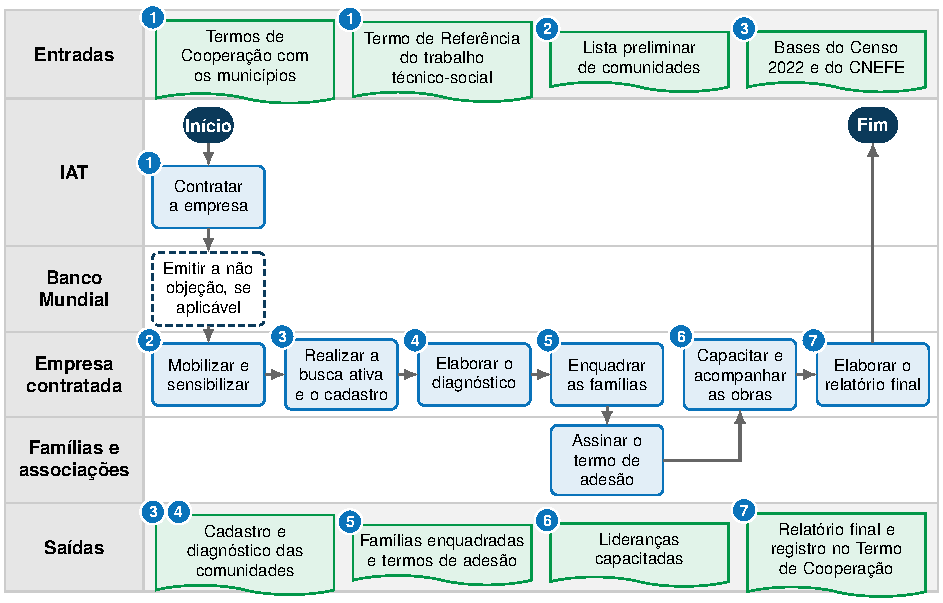
\includegraphics[width=15.96cm]{figuras/g-raias-3222.pdf}
  \fonteMOP{Fonte: IAT (2026).}
  % Texto alternativo: Fluxograma em raias do trabalho técnico-social, com uma raia por instituição, as etapas numeradas na raia do executor, as entradas no topo e as saídas na base.
\end{figure}

\phantomsection
\subsubsection*{4.1 Etapa 1: Contratação da empresa}

\textbf{Atividades:} elaboração do Termo de Referência, com escopo, produtos, prazos e perfil da equipe; publicação do edital; seleção da empresa; assinatura do contrato e emissão da ordem de serviço.

\textbf{Entradas:} Termos de Cooperação assinados com os municípios; lista preliminar de comunidades.

\textbf{Responsáveis:} IAT (executa e aprova); UGP e Banco Mundial (consultados, quando houver revisão prévia).

\textbf{Produto:} contrato assinado e ordem de serviço.

\phantomsection
\subsubsection*{4.2 Etapa 2: Mobilização e sensibilização}

\textbf{Atividades:} reuniões com as prefeituras, as associações e as lideranças; reuniões comunitárias, com linguagem acessível, para apresentação do Programa, estímulo à participação e reconhecimento do território; divulgação do Mecanismo de Queixas e Reclamações.

\textbf{Entradas:} contrato; agenda pactuada com as prefeituras.

\textbf{Responsáveis:} empresa contratada (executa); SEAB e prefeituras (consultadas); IAT (aprova).

\textbf{Produto:} plano de mobilização executado, com atas e listas de presença.

\phantomsection
\subsubsection*{4.3 Etapa 3: Busca ativa e cadastro domiciliar}

\textbf{Atividades:} visita a todos os domicílios da comunidade, inclusive em áreas remotas, sem dependência exclusiva de cadastros prévios; inventário social; cadastro domiciliar georreferenciado. O tratamento dos dados pessoais observa a Lei Geral de Proteção de Dados Pessoais (LGPD) e restringe-se às finalidades da ação (BRASIL, 2018).

\textbf{Entradas:} lista de comunidades; bases do Censo 2022 e do Cadastro Nacional de Endereços para Fins Estatísticos (CNEFE).

\textbf{Responsáveis:} empresa contratada (executa); IAT (aprova); SEAB (consultada).

\textbf{Produto:} cadastro domiciliar georreferenciado.

\phantomsection
\subsubsection*{4.4 Etapa 4: Diagnóstico coletivo e domiciliar}

\textbf{Atividades:} diagnóstico das formas atuais de abastecimento e de esgotamento sanitário, da demanda de água, da infraestrutura necessária e da viabilidade dos sistemas; levantamento das condições de cada domicílio para a solução de esgotamento sanitário; validação social das tecnologias propostas.

\textbf{Entradas:} cadastro domiciliar.

\textbf{Responsáveis:} empresa contratada (executa); IAT (aprova); SEAB (consultada).

\textbf{Produto:} diagnóstico por comunidade e por domicílio.

\phantomsection
\subsubsection*{4.5 Etapa 5: Enquadramento e adesão das famílias}

\textbf{Atividades:} aplicação dos critérios sociais, territoriais e técnicos de definição das famílias atendidas; assinatura do termo de adesão, com o compromisso de uso e manutenção adequados.

\textbf{Entradas:} diagnóstico; critérios de enquadramento aprovados pelo IAT.

\textbf{Responsáveis:} empresa contratada e famílias (executam); IAT (aprova).

\textbf{Produto:} lista de famílias enquadradas e termos de adesão assinados.

\phantomsection
\subsubsection*{4.6 Etapa 6: Educação sanitária e ambiental e acompanhamento}

\textbf{Atividades:} oficinas de educação sanitária e ambiental; capacitação das lideranças locais; apoio à organização comunitária e à constituição da associação; acompanhamento social das obras e da entrega dos sistemas.

\textbf{Entradas:} termos de adesão; cronograma das obras de abastecimento.

\textbf{Responsáveis:} empresa contratada (executa); IAT (aprova); prefeituras e SEAB (consultadas).

\textbf{Produto:} lideranças capacitadas, com listas de presença e certificados, e relatórios de acompanhamento.

\phantomsection
\subsubsection*{4.7 Etapa 7: Relatório final}

\textbf{Atividades:} consolidação dos resultados; elaboração do relatório final; registro da conclusão da etapa no Termo de Cooperação.

\textbf{Entradas:} produtos das Etapas 2 a 6.

\textbf{Responsáveis:} empresa contratada (executa); SEAB (consultada na validação); IAT (aprova).

\pendencia{A nota técnica prevê a validação conjunta do relatório final. Na matriz, a SEAB figura como C (consultada antes da aprovação), porque o Guia de Identidade Visual admite um único A por etapa; confirmar.}

\textbf{Produto:} relatório final aprovado.

\phantomsection
\subsubsection*{4.8 Modalidade de execução}

O item de custo é o trabalho técnico e social: 36 profissionais-mês a R\$~179.835,30, no total de R\$~6,47 milhões, com recursos do empréstimo do BIRD. A execução ocorre mediante licitação de serviços, conforme o Caderno AQ, e o número de lotes é definido no Plano de Aquisições.

\phantomsection
\addcontentsline{toc}{subsection}{5. Matriz de responsabilidades}
\subsection*{5. Matriz de responsabilidades}

O Quadro~\ref{raci-3222} apresenta o papel de cada parte em cada etapa.

\begin{quadro}[H]
  \caption{Matriz de responsabilidades do trabalho técnico-social}\label{raci-3222}
  \footnotesize\renewcommand{\arraystretch}{1.25}\setlength{\tabcolsep}{3pt}
  \begin{tabular}{>{\raggedright\arraybackslash}p{\dimexpr 0.2536\linewidth-2\tabcolsep\relax}>{\centering\arraybackslash}p{\dimexpr 0.0882\linewidth-2\tabcolsep\relax}>{\centering\arraybackslash}p{\dimexpr 0.0882\linewidth-2\tabcolsep\relax}>{\centering\arraybackslash}p{\dimexpr 0.0882\linewidth-2\tabcolsep\relax}>{\centering\arraybackslash}p{\dimexpr 0.0882\linewidth-2\tabcolsep\relax}>{\centering\arraybackslash}p{\dimexpr 0.0882\linewidth-2\tabcolsep\relax}>{\centering\arraybackslash}p{\dimexpr 0.0882\linewidth-2\tabcolsep\relax}>{\centering\arraybackslash}p{\dimexpr 0.0882\linewidth-2\tabcolsep\relax}>{\centering\arraybackslash}p{\dimexpr 0.1291\linewidth-2\tabcolsep\relax}}
    \rowcolor{azulEscuro}\textcolor{white}{\textbf{Parte}} & \textcolor{white}{\textbf{E1}} & \textcolor{white}{\textbf{E2}} & \textcolor{white}{\textbf{E3}} & \textcolor{white}{\textbf{E4}} & \textcolor{white}{\textbf{E5}} & \textcolor{white}{\textbf{E6}} & \textcolor{white}{\textbf{E7}} & \textcolor{white}{\textbf{Produto final}} \\
    IAT & \raci{R} \raci{A} & \raci{A} & \raci{A} & \raci{A} & \raci{A} & \raci{A} & \raci{A} & \raci{A} \\ \arrayrulecolor{cinza20}\hline
    \rowcolor{cinza5}SEAB & – & \raci{C} & \raci{C} & \raci{C} & \raci{C} & \raci{C} & \raci{C} & \raci{C} \\ \arrayrulecolor{cinza20}\hline
    Empresa contratada & – & \raci{R} & \raci{R} & \raci{R} & \raci{R} & \raci{R} & \raci{R} & \raci{R} \\ \arrayrulecolor{cinza20}\hline
    \rowcolor{cinza5}Prefeituras & \raci{I} & \raci{C} & \raci{I} & \raci{I} & \raci{I} & \raci{C} & \raci{I} & \raci{I} \\ \arrayrulecolor{cinza20}\hline
    Famílias e associações & – & \raci{C} & \raci{C} & \raci{C} & \raci{R} & \raci{C} & \raci{I} & \raci{I} \\ \arrayrulecolor{cinza20}\hline
    \rowcolor{cinza5}UGP & \raci{C} & \raci{I} & \raci{I} & \raci{I} & \raci{I} & \raci{I} & \raci{I} & \raci{I} \\ \arrayrulecolor{cinza20}\hline
    Banco Mundial & \raci{C} & – & – & – & – & – & – & – \\ \noalign{\global\arrayrulewidth=1pt}\arrayrulecolor{azulEscuro}\hline\noalign{\global\arrayrulewidth=0.4pt}
  \end{tabular}
  \fonteMOP{Fonte: IAT (2026).}
  \notaMOP{Nota: E1 a E7 correspondem às Etapas 1 a 7 do item 4. \raci{R} executa (pode haver mais de um); \raci{A} aprova ou valida o produto (um por etapa); \raci{C} é consultado previamente; \raci{I} é informado posteriormente. Produto final: cadastro, diagnóstico e termos de adesão das 83 comunidades.}
\end{quadro}

\phantomsection
\addcontentsline{toc}{subsection}{6. Metas, indicadores e comprovação}
\subsection*{6. Metas, indicadores e comprovação}

A meta física é expressa em profissionais-mês e concentra-se entre 2027 e 2030 (Quadro~\ref{metas-3222}), pois o diagnóstico deve estar concluído antes dos projetos e das obras.

\begin{quadro}[H]
  \caption{Metas anuais do trabalho técnico-social}\label{metas-3222}
  \footnotesize\renewcommand{\arraystretch}{1.25}\setlength{\tabcolsep}{3pt}
  \begin{tabular}{>{\raggedright\arraybackslash}p{\dimexpr 0.2095\linewidth-2\tabcolsep\relax}>{\raggedright\arraybackslash}p{\dimexpr 0.1268\linewidth-2\tabcolsep\relax}>{\raggedleft\arraybackslash}p{\dimexpr 0.0794\linewidth-2\tabcolsep\relax}>{\raggedleft\arraybackslash}p{\dimexpr 0.0794\linewidth-2\tabcolsep\relax}>{\raggedleft\arraybackslash}p{\dimexpr 0.0794\linewidth-2\tabcolsep\relax}>{\raggedleft\arraybackslash}p{\dimexpr 0.0794\linewidth-2\tabcolsep\relax}>{\raggedleft\arraybackslash}p{\dimexpr 0.0794\linewidth-2\tabcolsep\relax}>{\raggedleft\arraybackslash}p{\dimexpr 0.0794\linewidth-2\tabcolsep\relax}>{\raggedleft\arraybackslash}p{\dimexpr 0.0794\linewidth-2\tabcolsep\relax}>{\raggedleft\arraybackslash}p{\dimexpr 0.1081\linewidth-2\tabcolsep\relax}}
    \rowcolor{azulEscuro}\textcolor{white}{\textbf{Produto}} & \textcolor{white}{\textbf{Unidade}} & \centering\arraybackslash \textcolor{white}{\textbf{Ano 1}} & \centering\arraybackslash \textcolor{white}{\textbf{Ano 2}} & \centering\arraybackslash \textcolor{white}{\textbf{Ano 3}} & \centering\arraybackslash \textcolor{white}{\textbf{Ano 4}} & \centering\arraybackslash \textcolor{white}{\textbf{Ano 5}} & \centering\arraybackslash \textcolor{white}{\textbf{Ano 6}} & \centering\arraybackslash \textcolor{white}{\textbf{Ano 7}} & \centering\arraybackslash \textcolor{white}{\textbf{Total}} \\
    Trabalho técnico e social & prof.-mês & 6 & 12 & 12 & 6 & – & – & – & 36 \\ \noalign{\global\arrayrulewidth=1pt}\arrayrulecolor{azulEscuro}\hline\noalign{\global\arrayrulewidth=0.4pt}
  \end{tabular}
  \fonteMOP{Fonte: Planilha PSH\_CUSTO\_Consolidada, versão v2408 (PARANÁ, 2026).}
  \notaMOP{Nota: Ano 1 = 2027 e Ano 7 = 2033. Prof.-mês = profissionais-mês.}
\end{quadro}

O Quadro~\ref{ind-3222} reúne os indicadores de andamento da ação, apurados por comunidade.

\begin{quadro}[H]
  \caption{Indicadores do trabalho técnico-social}\label{ind-3222}
  \footnotesize\renewcommand{\arraystretch}{1.25}\setlength{\tabcolsep}{3pt}
  \begin{tabular}{>{\raggedright\arraybackslash}p{\dimexpr 0.3165\linewidth-2\tabcolsep\relax}>{\raggedright\arraybackslash}p{\dimexpr 0.1378\linewidth-2\tabcolsep\relax}>{\raggedleft\arraybackslash}p{\dimexpr 0.1102\linewidth-2\tabcolsep\relax}>{\raggedleft\arraybackslash}p{\dimexpr 0.1599\linewidth-2\tabcolsep\relax}>{\raggedright\arraybackslash}p{\dimexpr 0.2756\linewidth-2\tabcolsep\relax}}
    \rowcolor{azulEscuro}\textcolor{white}{\textbf{Indicador}} & \textcolor{white}{\textbf{Unidade}} & \centering\arraybackslash \textcolor{white}{\textbf{Linha de base (2025)}} & \centering\arraybackslash \textcolor{white}{\textbf{Meta}} & \textcolor{white}{\textbf{Frequência e fonte dos dados}} \\
    Comunidades com diagnóstico aprovado & comunidades & 0 & 83 & Por lote; IAT \\ \arrayrulecolor{cinza20}\hline
    \rowcolor{cinza5}Domicílios cadastrados & domicílios & 0 & 5.810 & Por lote; cadastro domiciliar \\ \arrayrulecolor{cinza20}\hline
    Famílias com termo de adesão assinado & famílias & 0 & a definir no diagnóstico & Por lote; IAT \\ \arrayrulecolor{cinza20}\hline
    \rowcolor{cinza5}Lideranças e moradores capacitados & pessoas & 0 & a definir no plano de trabalho & Semestral; listas de presença \\ \noalign{\global\arrayrulewidth=1pt}\arrayrulecolor{azulEscuro}\hline\noalign{\global\arrayrulewidth=0.4pt}
  \end{tabular}
  \fonteMOP{Fonte: IAT (2026).}
\end{quadro}

\pendencia{Definir as metas de famílias aderidas e de pessoas capacitadas no plano de trabalho da empresa contratada.}

Os critérios de aceite e as evidências constam do Quadro~\ref{aceite-3222}. O relatório final, aprovado pelo IAT após consulta à SEAB, constitui a evidência de conclusão de cada lote e registra a conclusão da etapa no Termo de Cooperação.

\begin{quadro}[H]
  \caption{Critérios de aceite e evidências do trabalho técnico-social}\label{aceite-3222}
  \footnotesize\renewcommand{\arraystretch}{1.25}\setlength{\tabcolsep}{5pt}
  \begin{tabular}{>{\raggedright\arraybackslash}p{\dimexpr 0.2150\linewidth-2\tabcolsep\relax}>{\raggedright\arraybackslash}p{\dimexpr 0.3386\linewidth-2\tabcolsep\relax}>{\raggedright\arraybackslash}p{\dimexpr 0.2921\linewidth-2\tabcolsep\relax}>{\raggedright\arraybackslash}p{\dimexpr 0.1543\linewidth-2\tabcolsep\relax}}
    \rowcolor{azulEscuro}\textcolor{white}{\textbf{Produto}} & \textcolor{white}{\textbf{Critério de aceite}} & \textcolor{white}{\textbf{Evidência de comprovação}} & \textcolor{white}{\textbf{Responsável pela validação}} \\
    Plano de trabalho & Metodologia, cronograma e equipe compatíveis com o Termo de Referência & Plano aprovado & IAT \\ \arrayrulecolor{cinza20}\hline
    \rowcolor{cinza5}Cadastro domiciliar & Todos os domicílios da comunidade visitados e georreferenciados; dados tratados conforme a LGPD & Base do cadastro; relatório de campo & IAT \\ \arrayrulecolor{cinza20}\hline
    Diagnóstico & Condições de abastecimento e de esgotamento sanitário descritas por comunidade e por domicílio & Relatório de diagnóstico & IAT \\ \arrayrulecolor{cinza20}\hline
    \rowcolor{cinza5}Termos de adesão & Assinados pelas famílias enquadradas & Termos assinados & IAT \\ \arrayrulecolor{cinza20}\hline
    Capacitação & Conteúdo do plano de educação sanitária e ambiental cumprido & Listas de presença e certificados & IAT \\ \arrayrulecolor{cinza20}\hline
    \rowcolor{cinza5}Relatório final & Consolida os produtos e é aprovado & Relatório final; registro no Termo de Cooperação & IAT, após consulta à SEAB \\ \noalign{\global\arrayrulewidth=1pt}\arrayrulecolor{azulEscuro}\hline\noalign{\global\arrayrulewidth=0.4pt}
  \end{tabular}
  \fonteMOP{Fonte: IAT (2026).}
\end{quadro}

\phantomsection
\addcontentsline{toc}{subsection}{7. Gestão de riscos e impactos ambientais e sociais}
\subsection*{7. Gestão de riscos e impactos ambientais e sociais}

A ação não envolve obras. Os riscos concentram-se na exclusão de famílias, na consulta inadequada a comunidades tradicionais, nas condições de trabalho da equipe de campo e no tratamento dos dados pessoais do cadastro. O Quadro~\ref{nas-3222} indica as NAS aplicáveis e as medidas; as NAS 3, 4, 5, 6 e 8 não se aplicam à ação.

\begin{quadro}[H]
  \caption{Aplicação das Normas Ambientais e Sociais ao trabalho técnico-social}\label{nas-3222}
  \footnotesize\renewcommand{\arraystretch}{1.25}\setlength{\tabcolsep}{5pt}
  \begin{tabular}{>{\raggedright\arraybackslash}p{\dimexpr 0.1874\linewidth-2\tabcolsep\relax}>{\raggedright\arraybackslash}p{\dimexpr 0.3716\linewidth-2\tabcolsep\relax}>{\raggedright\arraybackslash}p{\dimexpr 0.4410\linewidth-2\tabcolsep\relax}}
    \rowcolor{azulEscuro}\textcolor{white}{\textbf{NAS}} & \textcolor{white}{\textbf{Aplicação à ação}} & \textcolor{white}{\textbf{Medidas e instrumentos}} \\
    NAS 1 – Avaliação e gestão de riscos & Risco de exclusão de famílias vulneráveis ou de áreas remotas & Busca ativa em todos os domicílios; aplicação rigorosa dos critérios de vulnerabilidade social (MGAS) \\ \arrayrulecolor{cinza20}\hline
    \rowcolor{cinza5}NAS 2 – Condições de trabalho & Equipe de campo da empresa contratada & Cláusulas trabalhistas e de segurança nos deslocamentos; Procedimentos de Gestão de Mão de Obra \\ \arrayrulecolor{cinza20}\hline
    NAS 7 – Povos indígenas e comunidades tradicionais & Comunidades tradicionais nas áreas selecionadas & Consulta culturalmente adequada, com participação das lideranças (MGAS e PEPI) \\ \arrayrulecolor{cinza20}\hline
    \rowcolor{cinza5}NAS 10 – Engajamento das partes interessadas & Toda a ação, por constituir o principal canal de diálogo com as famílias & Reuniões com linguagem acessível; registro das consultas; divulgação e acompanhamento do Mecanismo de Queixas e Reclamações (PEPI e MQR) \\ \noalign{\global\arrayrulewidth=1pt}\arrayrulecolor{azulEscuro}\hline\noalign{\global\arrayrulewidth=0.4pt}
  \end{tabular}
  \fonteMOP{Fonte: IAT (2026), com base nos instrumentos do Caderno AS.}
  \notaMOP{Nota: o cadastro domiciliar observa a Lei Geral de Proteção de Dados Pessoais (BRASIL, 2018).}
\end{quadro}

\phantomsection
\addcontentsline{toc}{subsection}{8. Cronograma}
\subsection*{8. Cronograma}

A contratação ocorre em 2027; a mobilização, o cadastro e o diagnóstico, de 2027 a 2029; o enquadramento e as adesões, em 2028 e 2029; a educação sanitária e ambiental e o acompanhamento, de 2028 a 2030; e o relatório final, em 2030 (Figura~\ref{crono-3222}).

\begin{figure}[H]
  \centering
  \caption{Cronograma das etapas e das entregas do trabalho técnico-social}\label{crono-3222}
  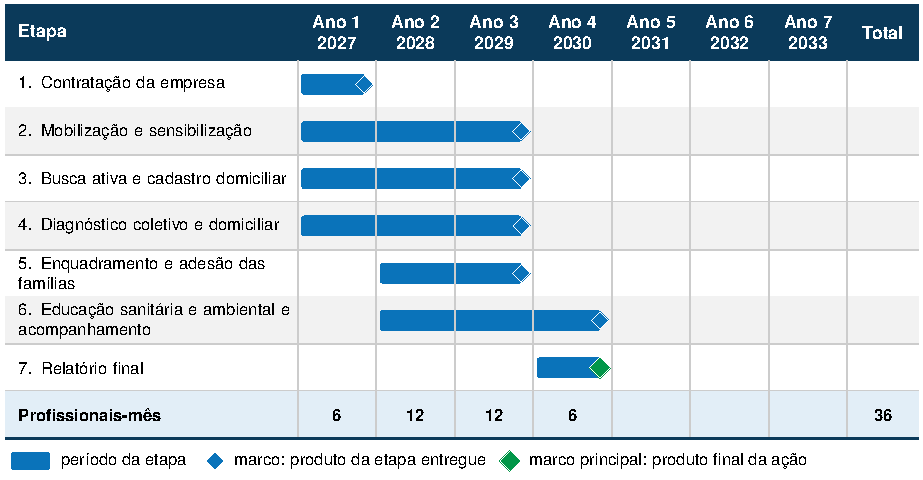
\includegraphics[width=15.64cm]{figuras/g-crono-3222.pdf}
  \fonteMOP{Fonte: IAT (2026), com quantidades da planilha PSH\_CUSTO\_Consolidada (PARANÁ, 2026).}
  % Texto alternativo: Cronograma anual de 2027 a 2033 com as etapas e as quantidades a entregar do trabalho técnico-social.
\end{figure}

\pendencia{O trabalho técnico-social encerra-se em 2030, e as obras de abastecimento e de esgotamento sanitário prosseguem até 2033. Avaliar se o acompanhamento social das obras de 2031 a 2033 requer recursos adicionais ou se será realizado pela equipe do IAT e pelas unidades regionais.}

\phantomsection
\addcontentsline{toc}{subsection}{9. Interfaces e dependências}
\subsection*{9. Interfaces e dependências}

A ação recebe dos modelos de gestão os municípios aderidos e os Termos de Cooperação e, da implantação dos sistemas de abastecimento, o cronograma das obras. Fornece o cadastro e as adesões que dão origem às associações, o diagnóstico que subsidia os projetos de abastecimento e a relação de domicílios sem esgotamento sanitário adequado (Figura~\ref{interf-3222}).

\begin{figure}[H]
  \centering
  \caption{Interfaces e dependências do trabalho técnico-social}\label{interf-3222}
  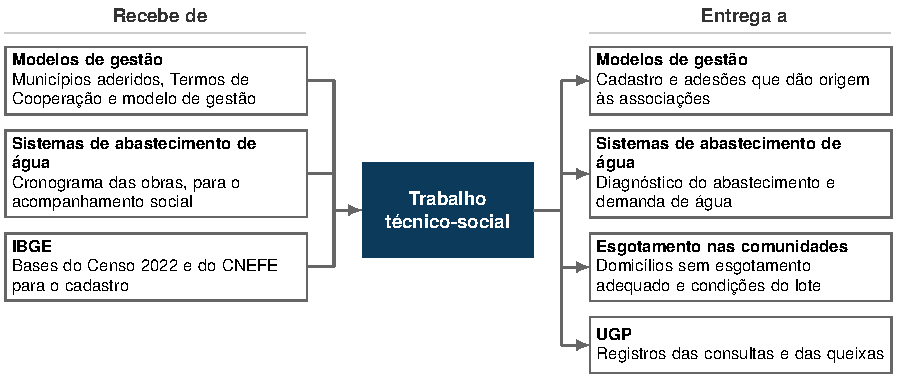
\includegraphics[width=15.30cm]{figuras/g-interf-3222.pdf}
  \fonteMOP{Fonte: IAT (2026).}
  % Texto alternativo: Diagrama das interfaces do trabalho técnico-social: insumos recebidos de outras partes do Programa e produtos entregues a elas.
\end{figure}

\phantomsection
\addcontentsline{toc}{subsection}{10. Documentos complementares}
\subsection*{10. Documentos complementares}

\begin{itemize}
  \item Termo de Referência do trabalho técnico-social (a elaborar);
  \item Termo de Cooperação entre o IAT e cada município;
  \item Plano de Engajamento das Partes Interessadas (PEPI) e Mecanismo de Queixas e Reclamações, no Caderno AS;
  \item Lei nº~13.709/2018 (Lei Geral de Proteção de Dados Pessoais);
  \item Programa Nacional de Saneamento Rural (BRASIL, 2019);
  \item Caderno AQ.
\end{itemize}

\acao{Ação 3.2.2.3 – Implantação e reabilitação dos sistemas coletivos de abastecimento de água}

\phantomsection
\addcontentsline{toc}{subsection}{1. Contextualização}
\subsection*{1. Contextualização}

A ação implanta ou reabilita 83 sistemas coletivos de abastecimento de água em comunidades rurais, com captação subterrânea por poço tubular profundo, desinfecção por cloração, reservação, rede de distribuição e ligações domiciliares com hidrômetro. Os sistemas atendem 5.810 domicílios, cerca de 16,3 mil pessoas, entre 2028 e 2033 (PARANÁ, 2026; IAT, 2026a).

No meio rural do Paraná, 99,59\% dos domicílios dispõem de água canalizada, segundo o Censo 2022, mas apenas 16,92\% do abastecimento provém de sistemas coletivos com tratamento completo (IAT, 2026a). Predominam nascentes e poços rasos escavados (cacimbas), em grande parte contaminados por agrotóxicos, metais e coliformes e sujeitos à redução de vazão nas estiagens recorrentes no Estado. O consumo de água contaminada está associado a doenças de veiculação hídrica, como diarreia, hepatite e esquistossomose.

Por essas razões, a ação adota a captação de água subterrânea por poço tubular profundo. A água subterrânea apresenta, em geral, melhor qualidade microbiológica e menor sensibilidade à variabilidade climática, o que, na maior parte dos casos, restringe o tratamento à desinfecção por cloração. A captação subterrânea tem também menor custo, menor prazo de implantação e menor impacto ambiental que a captação superficial, que requer barragem, adutora e estação de tratamento (IAT, 2026a).

A Figura~\ref{esquema-saa} apresenta os componentes de um sistema típico.

\begin{figure}[H]
  \centering
  \caption{Componentes de um sistema coletivo de abastecimento de água rural}\label{esquema-saa}
  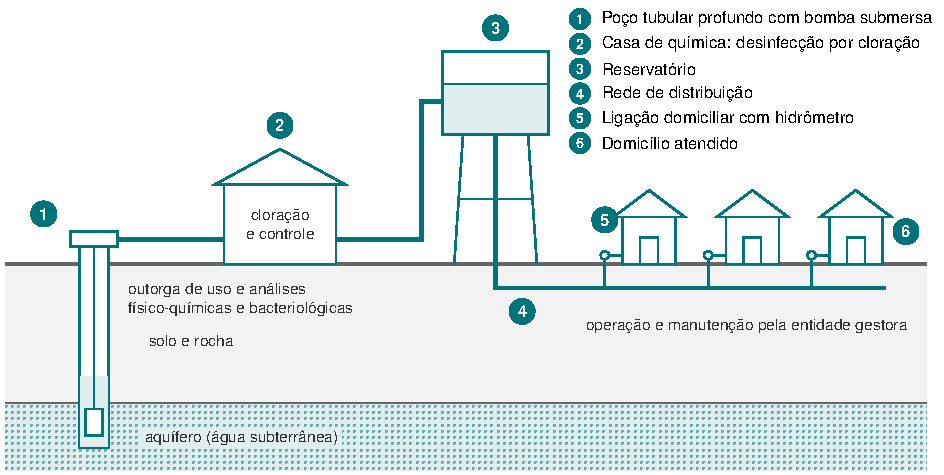
\includegraphics[width=15.98cm]{figuras/f-esquema-saa.pdf}
  \fonteMOP{Fonte: IAT (2026). Esquema ilustrativo, sem escala.}
  % Texto alternativo: Esquema em corte com poço tubular profundo, casa de química, reservatório elevado, rede de distribuição e domicílios com hidrômetro.
\end{figure}

A ação apoia-se na experiência do Programa Água no Campo, no qual o IAT perfura poços e implanta sistemas coletivos em comunidades não atendidas pelas companhias de saneamento. Desde 2019, o programa perfurou 801 poços, com investimento aproximado de R\$~12,3 milhões e cerca de 250 mil pessoas beneficiadas; no primeiro semestre de 2025, foram 39 poços em 21 municípios, para 1.253 famílias (IAT, 2026a). Os resultados esperados incluem a redução das doenças de veiculação hídrica e dos gastos públicos com saúde, a melhoria das condições de vida, o estímulo à permanência das famílias no campo e o fortalecimento da organização comunitária.

A ação constitui a principal contribuição do IAT ao indicador de pessoas atendidas com água gerida de forma segura: cerca de 16,3 mil das 59.780 pessoas previstas. As demais decorrem do Programa Sanepar Rural.

\textbf{Inclui:} estudos preliminares e regularização das áreas; locação, perfuração, teste de vazão, análises físico-químicas e bacteriológicas e outorga dos poços; projetos básico e executivo; licenciamento ambiental; obras da casa de química, do reservatório, das instalações eletromecânicas, da rede e das ligações com hidrômetro; reabilitação de sistemas existentes operados por associações; pré-operação, testes e capacitação dos operadores; e entrega à entidade gestora.

\textbf{Não inclui:} a supervisão independente das obras, o modelo de gestão, o trabalho técnico-social, o esgotamento sanitário e os sistemas do Programa Sanepar Rural, objeto de ações próprias.

\textbf{Valor previsto:} R\$~107,90 milhões (empréstimo BIRD: R\$~107,90 milhões; contrapartida: R\$~0,00 milhões), conforme a planilha PSH\_CUSTO\_Consolidada.

\phantomsection
\addcontentsline{toc}{subsection}{2. Área de atuação}
\subsection*{2. Área de atuação}

A ação abrange todo o Estado, nas Microrregiões de Água e Esgoto, e restringe-se às comunidades que atendem aos critérios de seleção (Figura~\ref{selecao-comunidades}). O primeiro critério é o adensamento: comunidade ou conjunto de comunidades com 70 ou mais domicílios ocupados, número mínimo que viabiliza o modelo de gestão.

O segundo critério é o desempenho do município no IPDM, que varia de 0 a 1 e classifica os municípios em quatro estratos: baixo (0 a menos de 0,4), médio baixo (0,4 a menos de 0,6), médio (0,6 a menos de 0,8) e alto (0,8 a 1,0). A ação restringe-se aos municípios de médio baixo e de médio desempenho.

Consideram-se, ainda, as solicitações de perfuração de poços já encaminhadas pelos municípios ao IAT e a existência de associações de moradores que operam sistemas com necessidade de complementação ou melhoria. Por fim, a comunidade somente prossegue para a implantação na ausência de impedimentos à perfuração: disponibilidade hídrica insuficiente no aquífero, condições geológicas que inviabilizem a obra, falhas geológicas com risco de contaminação ou de interrupção do fluxo, contaminantes que comprometam a potabilidade ou restrições legais e ambientais (IAT, 2026a).

\begin{figure}[H]
  \centering
  \caption{Critérios de seleção das comunidades atendidas com água}\label{selecao-comunidades}
  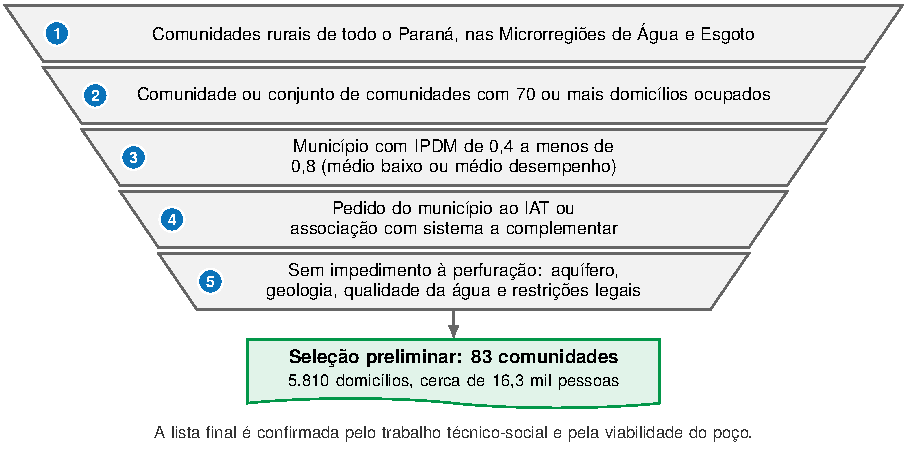
\includegraphics[width=15.37cm]{figuras/f-selecao-comunidades.pdf}
  \fonteMOP{Fonte: IAT (2026), com base em IAT (2026a).}
  % Texto alternativo: Funil com os cinco critérios de seleção das comunidades, que resulta na seleção preliminar de 83 comunidades e 5.810 domicílios.
\end{figure}

\pendencia{Justificar a exclusão dos municípios de baixo e de alto desempenho no IPDM. O Banco Mundial costuma questionar a exclusão de municípios mais vulneráveis.}

A aplicação preliminar dos critérios indicou 83 comunidades, com 5.810 domicílios, considerada a média de 70 domicílios por comunidade e de 2,8 habitantes por domicílio (Censo 2022). As áreas de maior concentração de domicílios rurais e os municípios consorciados ao CISPAR constam da Figura~\ref{mapa}. A lista final é confirmada pelo trabalho técnico-social e pela viabilidade do poço (Etapa 2).

\pendencia{O Acordo de Empréstimo, item (j)(vii) das definições, exige a identificação das áreas rurais da Parte 3.2. Anexar a lista das 83 comunidades selecionadas, com município e coordenadas, ou o mapa com a respectiva localização.}

\phantomsection
\addcontentsline{toc}{subsection}{3. Arranjo institucional e partes interessadas}
\subsection*{3. Arranjo institucional e partes interessadas}

A ação é coordenada pelo IAT, por meio da DISAR, responsável pelo planejamento, pela contratação, pela fiscalização e pelo recebimento dos sistemas. No próprio IAT, a Diretoria de Licenciamento e Outorga emite a outorga de direito de uso de recursos hídricos e as licenças ambientais. As prefeituras apoiam a regularização das áreas e a articulação local, a entidade gestora recebe e opera cada sistema, e a UGP acompanha a execução e consolida o reporte ao Banco Mundial.

\begin{itemize}
  \item \textbf{Coexecutora:} SEAB, na implementação local junto às comunidades;
  \item \textbf{Intervenientes:} prefeituras; entidades gestoras; empresas contratadas para projetos e obras; laboratórios contratados para as análises de potabilidade; empresa supervisora das obras;
  \item \textbf{Público envolvido:} proprietários das áreas do poço, do reservatório e da rede; moradores das comunidades.
\end{itemize}

\pendencia{O MOP de março e a nota técnica preveem a participação da instituição parceira da área rural na implementação local, sem detalhar o seu papel nesta ação. Detalhar a atuação da SEAB.}

Os beneficiários diretos são os moradores dos 5.810 domicílios ligados aos sistemas, cerca de 16,3 mil pessoas, selecionados pelos critérios do item 2. Os beneficiários indiretos são os municípios, com a redução de gastos com saúde, e a população do entorno, que deixa de depender de fontes contaminadas.

\phantomsection
\addcontentsline{toc}{subsection}{4. Processo de execução operacional}
\subsection*{4. Processo de execução operacional}

A implantação de cada sistema compreende seis etapas (Figura~\ref{raias-3223}). Duas premissas aplicam-se a todas: as comunidades atendidas são confirmadas pelo trabalho técnico-social, e o modelo de gestão é pactuado antes das obras. O produto final de cada sistema é o Termo de Recebimento Definitivo (TRD), emitido pelo IAT após o aceite da entidade gestora.

\begin{figure}[H]
  \centering
  \caption{Fluxograma da implantação dos sistemas coletivos de abastecimento de água: entradas, etapas por responsável e saídas}\label{raias-3223}
  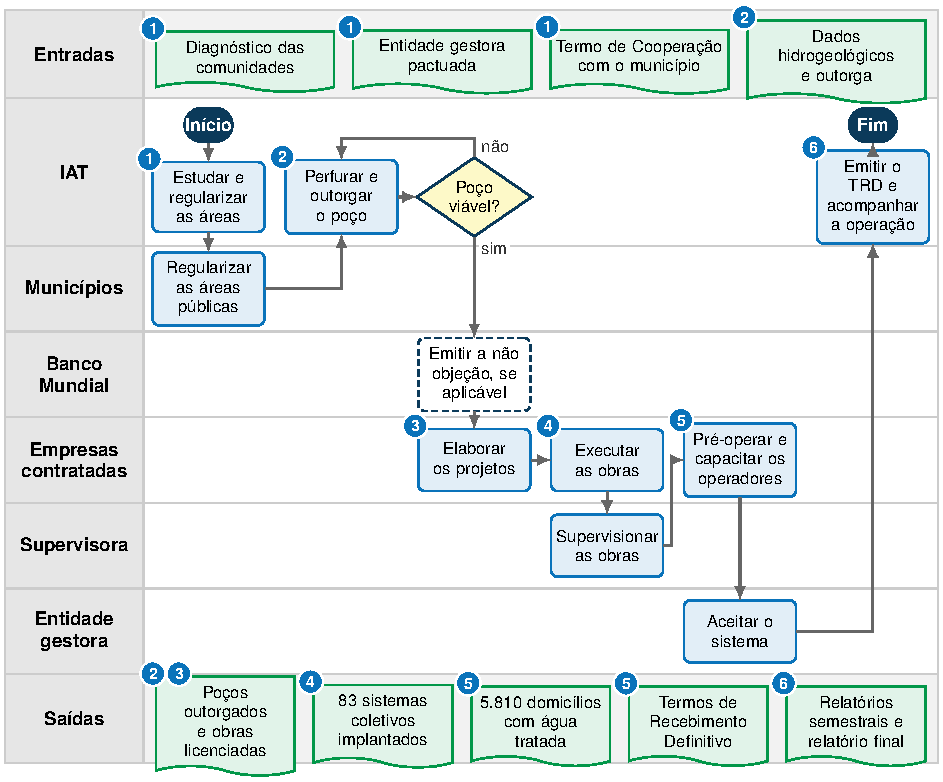
\includegraphics[width=15.96cm]{figuras/g-raias-3223.pdf}
  \fonteMOP{Fonte: IAT (2026).}
  % Texto alternativo: Fluxograma em raias da implantação dos sistemas coletivos de abastecimento de água, com uma raia por instituição, as etapas numeradas na raia do executor, as entradas no topo e as saídas na base.
\end{figure}

\phantomsection
\subsubsection*{4.1 Etapa 1: Estudos preliminares e regularização das áreas}

\textbf{Atividades:} estudos de viabilidade técnica, social e ambiental; levantamento de campo geológico e hidrogeológico; verificação da titularidade e da situação fundiária das áreas do poço, do reservatório e das demais estruturas; formalização da doação, da cessão ou da servidão das áreas, com anuência do proprietário; anteprojeto e investigação social. A Figura~\ref{captacao} apresenta a sequência das Etapas 1 a 3.

\begin{figure}[H]
  \centering
  \caption{Captação subterrânea, projeto e licenciamento (Etapas 1 a 3)}\label{captacao}
  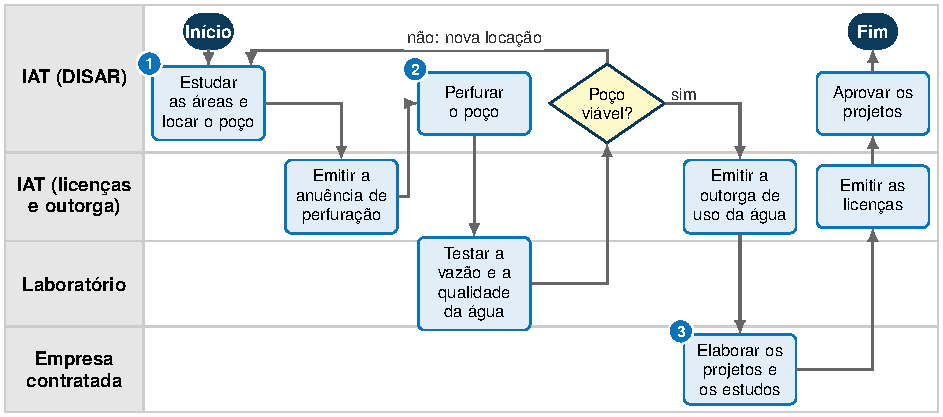
\includegraphics[width=15.96cm]{figuras/f-captacao.pdf}
  \fonteMOP{Fonte: IAT (2026), com base em IAT (2026b).}
  % Texto alternativo: Fluxograma em raias da DISAR, da área de licenciamento e outorga do IAT, do laboratório e da empresa contratada, com a decisão sobre a viabilidade do poço.
\end{figure}

\textbf{Entradas:} diagnóstico da comunidade (trabalho técnico-social); entidade gestora pactuada; Termo de Cooperação.

\textbf{Responsáveis:} IAT (executa e aprova); prefeituras (executam a regularização das áreas públicas); proprietários (consultados).

\textbf{Produto:} áreas regularizadas e anteprojeto aprovado.

\phantomsection
\subsubsection*{4.2 Etapa 2: Perfuração e outorga do poço}

\textbf{Atividades:} locação do poço e projeto construtivo; anuência prévia de perfuração; perfuração conforme as normas técnicas de projeto e construção de poços; teste de vazão; análises físico-químicas e bacteriológicas da água; outorga de direito de uso. Em caso de vazão ou qualidade insuficientes, o IAT procede a nova locação ou substitui a comunidade por outra que atenda aos critérios. O IAT dispõe de equipes próprias de perfuração, com equipamentos e equipe técnica para mais de 150 poços por ano (IAT, 2026a).

\textbf{Entradas:} áreas regularizadas; estudo hidrogeológico.

\textbf{Responsáveis:} equipe de perfuração do IAT ou empresa contratada (executa); laboratório contratado (análises); IAT (aprova e emite a outorga).

\textbf{Produto:} poço perfurado, testado e outorgado.

\pendencia{A nota técnica prevê a perfuração dos poços pelas equipes do IAT; o MOP de março previa a contratação integrada do poço. Definir o responsável pela perfuração.}

\phantomsection
\subsubsection*{4.3 Etapa 3: Contratação integrada, projetos e licenças}

\textbf{Atividades:} contratação integrada, na qual a mesma empresa elabora os projetos executivos e executa as obras; projetos básico e executivo da casa de química, do reservatório, das instalações eletromecânicas, da rede e das ligações; aprovação dos projetos pelo IAT; estudos ambientais e sociais e obtenção das licenças. As obras iniciam-se somente após a emissão da outorga e das licenças.

\textbf{Entradas:} poço outorgado; vazão e qualidade da água; anteprojeto.

\textbf{Responsáveis:} IAT (contrata, aprova os projetos e emite as licenças); empresa contratada (elabora os projetos); Banco Mundial (consultado, quando houver revisão prévia).

\textbf{Produto:} projetos aprovados e licenças emitidas.

\pendencia{O MOP define “contratação integrada” como aquela em que o contratado elabora o projeto executivo e executa a obra, o que corresponde à contratação semi-integrada da Lei nº~14.133/2021 (art. 6º, XXXIII). Definir o regime e verificar a compatibilidade com o Regulamento de Aquisições do Banco Mundial.}

\phantomsection
\subsubsection*{4.4 Etapa 4: Execução das obras}

\textbf{Atividades:} a obra é acompanhada em três níveis (Figura~\ref{obras}): o executor constrói conforme o projeto e instala hidrômetro em cada ligação domiciliar; a supervisora acompanha a execução e registra o andamento em relatórios mensais; e a fiscalização do IAT verifica a conformidade com o projeto e as normas. Constatada não conformidade, o executor procede à correção, e a obra é submetida a nova verificação. Atestada a conformidade, o IAT emite o atesto de recebimento, acompanhado dos laudos de vistoria e do projeto \textit{as built}.

\begin{figure}[H]
  \centering
  \caption{Execução, supervisão e fiscalização das obras, por responsável}\label{obras}
  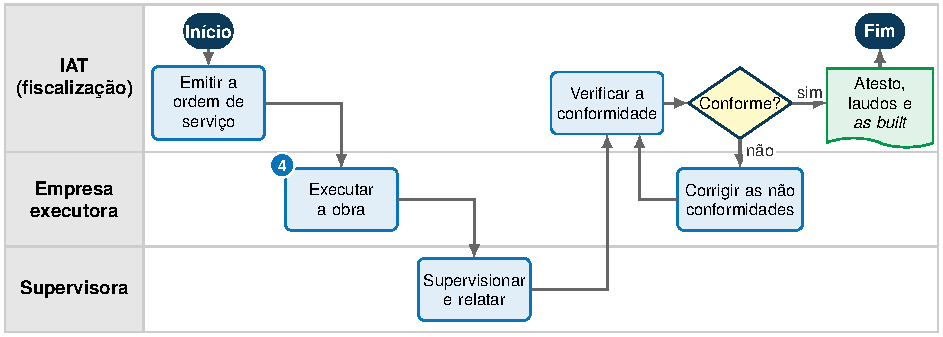
\includegraphics[width=15.96cm]{figuras/f-obras.pdf}
  \fonteMOP{Fonte: IAT (2026), com base em IAT (2026b).}
  % Texto alternativo: Fluxograma em raias da fiscalização do IAT, da empresa executora e da supervisora, com a decisão de conformidade e a correção das não conformidades.
\end{figure}

\textbf{Entradas:} projetos aprovados; outorga e licenças; ordem de serviço.

\textbf{Responsáveis:} empresa contratada (executa); supervisora (acompanha); IAT (fiscaliza e aprova); prefeituras (consultadas).

\textbf{Produto:} sistema implantado, com atesto de recebimento, laudos de vistoria e projeto \textit{as built}.

\pendencia{No MOP de março, a quantidade de hidrômetros consta como “XXX”. Pela meta de domicílios, são 5.810 hidrômetros, um por ligação; confirmar.}

\phantomsection
\subsubsection*{4.5 Etapa 5: Pré-operação, capacitação e entrega}

\textbf{Atividades:} pré-operação e testes de funcionamento; capacitação dos operadores locais, conforme o Plano de Operação e Manutenção; reunião técnica de entrega com a comunidade e a entidade gestora; aceite da entidade gestora; emissão do TRD (Figura~\ref{entrega}).

\begin{figure}[H]
  \centering
  \caption{Transferência, operação e encerramento dos sistemas de abastecimento}\label{entrega}
  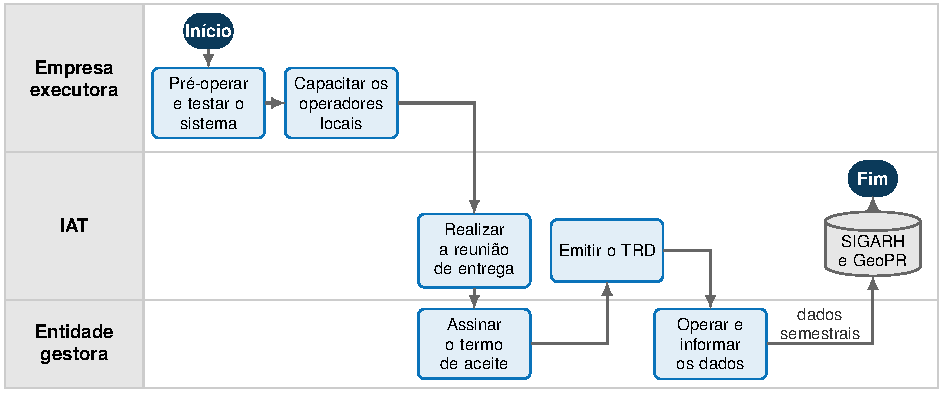
\includegraphics[width=15.96cm]{figuras/f-entrega.pdf}
  \fonteMOP{Fonte: IAT (2026), com base em IAT (2026b).}
  % Texto alternativo: Fluxograma em raias da empresa executora, do IAT e da entidade gestora, da pré-operação ao registro dos dados de operação no SIGARH e no GeoPR.
\end{figure}

\textbf{Entradas:} sistema implantado; entidade gestora constituída.

\textbf{Responsáveis:} empresa contratada (pré-operação e capacitação); entidade gestora (aceita o sistema); IAT (aprova e emite o TRD).

\textbf{Produto:} Termo de Recebimento Definitivo e operadores capacitados.

\phantomsection
\subsubsection*{4.6 Etapa 6: Acompanhamento pós-implantação e encerramento}

\textbf{Atividades:} suporte técnico pós-implantação; avaliação semestral de desempenho; acompanhamento da qualidade da água distribuída, conforme o padrão de potabilidade (BRASIL, 2021); registro dos dados no SIGARH e no GeoPR; relatório final e prestação de contas.

\textbf{Entradas:} TRD; dados de operação informados pela entidade gestora.

\textbf{Responsáveis:} IAT (executa); entidade gestora (informa os dados de operação); UGP (valida o relatório final).

\textbf{Produto:} relatórios semestrais de desempenho e relatório final.

\phantomsection
\subsubsection*{4.7 Modalidade de execução}

O item de custo é o de sistemas coletivos de abastecimento de água: 83 sistemas a R\$~1,3 milhão, no total de R\$~107,90 milhões, com recursos do empréstimo do BIRD. Os projetos executivos e as obras são contratados mediante licitação, em regime de contratação integrada, conforme o Caderno AQ; os ensaios laboratoriais de potabilidade também são licitados.

Os estudos preliminares, a regularização das áreas e a outorga são executados diretamente pelo IAT. A perfuração pode ser executada pelas equipes do IAT ou incluída na contratação das obras.

\pendencia{A nota técnica estima R\$~1,4 milhão por sistema; prevalece o valor da planilha de custos (R\$~1,3 milhão).}

\phantomsection
\addcontentsline{toc}{subsection}{5. Matriz de responsabilidades}
\subsection*{5. Matriz de responsabilidades}

O Quadro~\ref{raci-3223} apresenta o papel de cada parte em cada etapa.

\begin{quadro}[H]
  \caption{Matriz de responsabilidades da implantação dos sistemas coletivos de abastecimento de água}\label{raci-3223}
  \footnotesize\renewcommand{\arraystretch}{1.25}\setlength{\tabcolsep}{3pt}
  \begin{tabular}{>{\raggedright\arraybackslash}p{\dimexpr 0.2536\linewidth-2\tabcolsep\relax}>{\centering\arraybackslash}p{\dimexpr 0.0882\linewidth-2\tabcolsep\relax}>{\centering\arraybackslash}p{\dimexpr 0.0882\linewidth-2\tabcolsep\relax}>{\centering\arraybackslash}p{\dimexpr 0.0882\linewidth-2\tabcolsep\relax}>{\centering\arraybackslash}p{\dimexpr 0.0882\linewidth-2\tabcolsep\relax}>{\centering\arraybackslash}p{\dimexpr 0.0882\linewidth-2\tabcolsep\relax}>{\centering\arraybackslash}p{\dimexpr 0.0882\linewidth-2\tabcolsep\relax}>{\centering\arraybackslash}p{\dimexpr 0.2173\linewidth-2\tabcolsep\relax}}
    \rowcolor{azulEscuro}\textcolor{white}{\textbf{Parte}} & \textcolor{white}{\textbf{E1}} & \textcolor{white}{\textbf{E2}} & \textcolor{white}{\textbf{E3}} & \textcolor{white}{\textbf{E4}} & \textcolor{white}{\textbf{E5}} & \textcolor{white}{\textbf{E6}} & \textcolor{white}{\textbf{Produto final}} \\
    IAT & \raci{R} \raci{A} & \raci{R} \raci{A} & \raci{A} & \raci{A} & \raci{A} & \raci{R} & \raci{R} \raci{A} \\ \arrayrulecolor{cinza20}\hline
    \rowcolor{cinza5}Prefeituras & \raci{R} & \raci{I} & \raci{C} & \raci{C} & \raci{C} & \raci{I} & \raci{I} \\ \arrayrulecolor{cinza20}\hline
    Empresas contratadas & – & \raci{R} & \raci{R} & \raci{R} & \raci{R} & – & – \\ \arrayrulecolor{cinza20}\hline
    \rowcolor{cinza5}Supervisora & – & – & – & \raci{R} & \raci{C} & – & – \\ \arrayrulecolor{cinza20}\hline
    Entidade gestora & \raci{C} & \raci{I} & \raci{C} & \raci{I} & \raci{R} & \raci{R} & \raci{R} \\ \arrayrulecolor{cinza20}\hline
    \rowcolor{cinza5}UGP & \raci{I} & \raci{I} & \raci{I} & \raci{I} & \raci{I} & \raci{A} & \raci{I} \\ \arrayrulecolor{cinza20}\hline
    Banco Mundial & – & – & \raci{C} & – & – & \raci{I} & \raci{I} \\ \noalign{\global\arrayrulewidth=1pt}\arrayrulecolor{azulEscuro}\hline\noalign{\global\arrayrulewidth=0.4pt}
  \end{tabular}
  \fonteMOP{Fonte: IAT (2026).}
  \notaMOP{Nota: E1 a E6 correspondem às Etapas 1 a 6 do item 4. \raci{R} executa (pode haver mais de um); \raci{A} aprova ou valida o produto (um por etapa); \raci{C} é consultado previamente; \raci{I} é informado posteriormente. Produto final: sistemas em operação, com Termo de Recebimento Definitivo.}
\end{quadro}

\phantomsection
\addcontentsline{toc}{subsection}{6. Metas, indicadores e comprovação}
\subsection*{6. Metas, indicadores e comprovação}

O Quadro~\ref{metas-3223} distribui os 83 sistemas ao longo do Programa, com os domicílios ligados e as pessoas atendidas em cada ano.

\begin{quadro}[H]
  \caption{Metas anuais da implantação dos sistemas coletivos de abastecimento de água}\label{metas-3223}
  \footnotesize\renewcommand{\arraystretch}{1.25}\setlength{\tabcolsep}{3pt}
  \begin{tabular}{>{\raggedright\arraybackslash}p{\dimexpr 0.2095\linewidth-2\tabcolsep\relax}>{\raggedright\arraybackslash}p{\dimexpr 0.1268\linewidth-2\tabcolsep\relax}>{\raggedleft\arraybackslash}p{\dimexpr 0.0794\linewidth-2\tabcolsep\relax}>{\raggedleft\arraybackslash}p{\dimexpr 0.0794\linewidth-2\tabcolsep\relax}>{\raggedleft\arraybackslash}p{\dimexpr 0.0794\linewidth-2\tabcolsep\relax}>{\raggedleft\arraybackslash}p{\dimexpr 0.0794\linewidth-2\tabcolsep\relax}>{\raggedleft\arraybackslash}p{\dimexpr 0.0794\linewidth-2\tabcolsep\relax}>{\raggedleft\arraybackslash}p{\dimexpr 0.0794\linewidth-2\tabcolsep\relax}>{\raggedleft\arraybackslash}p{\dimexpr 0.0794\linewidth-2\tabcolsep\relax}>{\raggedleft\arraybackslash}p{\dimexpr 0.1081\linewidth-2\tabcolsep\relax}}
    \rowcolor{azulEscuro}\textcolor{white}{\textbf{Produto}} & \textcolor{white}{\textbf{Unidade}} & \centering\arraybackslash \textcolor{white}{\textbf{Ano 1}} & \centering\arraybackslash \textcolor{white}{\textbf{Ano 2}} & \centering\arraybackslash \textcolor{white}{\textbf{Ano 3}} & \centering\arraybackslash \textcolor{white}{\textbf{Ano 4}} & \centering\arraybackslash \textcolor{white}{\textbf{Ano 5}} & \centering\arraybackslash \textcolor{white}{\textbf{Ano 6}} & \centering\arraybackslash \textcolor{white}{\textbf{Ano 7}} & \centering\arraybackslash \textcolor{white}{\textbf{Total}} \\
    Sistemas coletivos de abastecimento de água & sistemas & – & 5 & 10 & 20 & 20 & 18 & 10 & 83 \\ \arrayrulecolor{cinza20}\hline
    \rowcolor{cinza5}Domicílios ligados & domicílios & – & 350 & 700 & 1.400 & 1.400 & 1.260 & 700 & 5.810 \\ \arrayrulecolor{cinza20}\hline
    Pessoas atendidas & pessoas & – & 980 & 1.960 & 3.920 & 3.920 & 3.528 & 1.960 & 16.268 \\ \noalign{\global\arrayrulewidth=1pt}\arrayrulecolor{azulEscuro}\hline\noalign{\global\arrayrulewidth=0.4pt}
  \end{tabular}
  \fonteMOP{Fonte: Planilha PSH\_CUSTO\_Consolidada, versão v2408 (PARANÁ, 2026).}
  \notaMOP{Nota: Ano 1 = 2027 e Ano 7 = 2033. Domicílios: 70 por sistema; pessoas: 2,8 por domicílio (Censo 2022).}
\end{quadro}

Os indicadores constam do Quadro~\ref{ind-3223}. O indicador de pessoas atendidas com água gerida de forma segura corresponde ao número acumulado de domicílios ligados aos sistemas multiplicado por 2,8, com desagregação por sexo e para jovens de 15 a 24 anos. Considera-se gerida de forma segura a água proveniente de fonte melhorada, disponível no domicílio por pelo menos 12 horas diárias e isenta de contaminação fecal e de contaminação química prioritária.

\begin{quadro}[H]
  \caption{Indicadores da implantação dos sistemas coletivos de abastecimento de água}\label{ind-3223}
  \footnotesize\renewcommand{\arraystretch}{1.25}\setlength{\tabcolsep}{3pt}
  \begin{tabular}{>{\raggedright\arraybackslash}p{\dimexpr 0.3165\linewidth-2\tabcolsep\relax}>{\raggedright\arraybackslash}p{\dimexpr 0.1378\linewidth-2\tabcolsep\relax}>{\raggedleft\arraybackslash}p{\dimexpr 0.1102\linewidth-2\tabcolsep\relax}>{\raggedleft\arraybackslash}p{\dimexpr 0.1599\linewidth-2\tabcolsep\relax}>{\raggedright\arraybackslash}p{\dimexpr 0.2756\linewidth-2\tabcolsep\relax}}
    \rowcolor{azulEscuro}\textcolor{white}{\textbf{Indicador}} & \textcolor{white}{\textbf{Unidade}} & \centering\arraybackslash \textcolor{white}{\textbf{Linha de base (2025)}} & \centering\arraybackslash \textcolor{white}{\textbf{Meta}} & \textcolor{white}{\textbf{Frequência e fonte dos dados}} \\
    Sistemas implantados com Termo de Recebimento Definitivo & sistemas & 0 & 83 & Semestral; IAT \\ \arrayrulecolor{cinza20}\hline
    \rowcolor{cinza5}Domicílios atendidos com sistema coletivo de abastecimento & domicílios & 0 & 5.810 & Anual; IAT e entidades gestoras \\ \arrayrulecolor{cinza20}\hline
    Pessoas atendidas com água gerida de forma segura (parcela do indicador do componente) & pessoas & 0 & 16.268 & Anual; IAT, com desagregação por sexo e jovens \\ \arrayrulecolor{cinza20}\hline
    \rowcolor{cinza5}Análises de entrega conformes ao padrão de potabilidade & \% das análises & – & 100 & Na entrega e semestral; laudos laboratoriais \\ \noalign{\global\arrayrulewidth=1pt}\arrayrulecolor{azulEscuro}\hline\noalign{\global\arrayrulewidth=0.4pt}
  \end{tabular}
  \fonteMOP{Fonte: IAT (2026).}
\end{quadro}

Os critérios de aceite e as evidências de cada produto constam do Quadro~\ref{aceite-3223}. A evidência de conclusão de cada sistema é o TRD; no encerramento, o relatório final é validado pela UGP e apresentado ao Banco Mundial.

\begin{quadro}[H]
  \caption{Critérios de aceite e evidências da implantação dos sistemas coletivos de abastecimento de água}\label{aceite-3223}
  \footnotesize\renewcommand{\arraystretch}{1.25}\setlength{\tabcolsep}{5pt}
  \begin{tabular}{>{\raggedright\arraybackslash}p{\dimexpr 0.2150\linewidth-2\tabcolsep\relax}>{\raggedright\arraybackslash}p{\dimexpr 0.3386\linewidth-2\tabcolsep\relax}>{\raggedright\arraybackslash}p{\dimexpr 0.2921\linewidth-2\tabcolsep\relax}>{\raggedright\arraybackslash}p{\dimexpr 0.1543\linewidth-2\tabcolsep\relax}}
    \rowcolor{azulEscuro}\textcolor{white}{\textbf{Produto}} & \textcolor{white}{\textbf{Critério de aceite}} & \textcolor{white}{\textbf{Evidência de comprovação}} & \textcolor{white}{\textbf{Responsável pela validação}} \\
    Áreas regularizadas & Titularidade comprovada; doação, cessão ou servidão formalizada & Matrícula ou termo de cessão; anuência do proprietário & IAT \\ \arrayrulecolor{cinza20}\hline
    \rowcolor{cinza5}Poço perfurado & Construído conforme o projeto construtivo e as normas técnicas & Relatório de perfuração; laudo de vistoria; atesto de recebimento & IAT \\ \arrayrulecolor{cinza20}\hline
    Vazão e qualidade & Vazão compatível com a demanda e água conforme o padrão de potabilidade & Teste de vazão; laudos físico-químicos e bacteriológicos & IAT \\ \arrayrulecolor{cinza20}\hline
    \rowcolor{cinza5}Outorga & Outorga de direito de uso emitida & Ato de outorga & IAT \\ \arrayrulecolor{cinza20}\hline
    Projetos e licenças & Projetos básico e executivo aprovados; licenças emitidas & Parecer de aprovação; licenças & IAT \\ \arrayrulecolor{cinza20}\hline
    \rowcolor{cinza5}Sistema implantado & Obra conforme o projeto e as normas; um hidrômetro por ligação & Relatórios de supervisão e de fiscalização; laudos; \textit{as built} & IAT \\ \arrayrulecolor{cinza20}\hline
    Operadores capacitados & Capacitação conforme o Plano de Operação e Manutenção & Listas de presença e certificados & IAT \\ \arrayrulecolor{cinza20}\hline
    \rowcolor{cinza5}Sistema entregue & Testes aprovados, aceite da entidade gestora e abastecimento por pelo menos 12 horas diárias & Termo de aceite; Termo de Recebimento Definitivo & IAT \\ \noalign{\global\arrayrulewidth=1pt}\arrayrulecolor{azulEscuro}\hline\noalign{\global\arrayrulewidth=0.4pt}
  \end{tabular}
  \fonteMOP{Fonte: IAT (2026).}
\end{quadro}

\phantomsection
\addcontentsline{toc}{subsection}{7. Gestão de riscos e impactos ambientais e sociais}
\subsection*{7. Gestão de riscos e impactos ambientais e sociais}

A ação envolve obras de pequeno porte, dispersas no território estadual. Os principais riscos são a contaminação do aquífero, os impactos temporários das obras (ruído, poeira, resíduos e erosão localizada), os acidentes de trabalho, os conflitos relativos à posse das áreas e ao uso da água e a exclusão de famílias vulneráveis. O Quadro~\ref{nas-3223} indica as NAS aplicáveis e as respectivas medidas.

A NAS 9 não se aplica ao Programa, e as medidas detalhadas constam do Caderno AS.

\begin{quadro}[H]
  \caption{Aplicação das Normas Ambientais e Sociais à implantação dos sistemas coletivos de abastecimento de água}\label{nas-3223}
  \footnotesize\renewcommand{\arraystretch}{1.25}\setlength{\tabcolsep}{5pt}
  \begin{tabular}{>{\raggedright\arraybackslash}p{\dimexpr 0.1874\linewidth-2\tabcolsep\relax}>{\raggedright\arraybackslash}p{\dimexpr 0.3716\linewidth-2\tabcolsep\relax}>{\raggedright\arraybackslash}p{\dimexpr 0.4410\linewidth-2\tabcolsep\relax}}
    \rowcolor{azulEscuro}\textcolor{white}{\textbf{NAS}} & \textcolor{white}{\textbf{Aplicação à ação}} & \textcolor{white}{\textbf{Medidas e instrumentos}} \\
    NAS 1 – Avaliação e gestão de riscos & Obras de captação, reservação e distribuição em cada comunidade & Triagem socioambiental de cada sistema; licenciamento; plano ambiental e social da obra (MGAS) \\ \arrayrulecolor{cinza20}\hline
    \rowcolor{cinza5}NAS 2 – Condições de trabalho & Equipes de perfuração e de obras & Uso de equipamento de proteção individual (EPI); treinamento de segurança; código de conduta (Procedimentos de Gestão de Mão de Obra) \\ \arrayrulecolor{cinza20}\hline
    NAS 3 – Eficiência de recursos e prevenção da poluição & Uso da água subterrânea; risco de contaminação do aquífero; resíduos e fluidos de perfuração & Outorga e hidrometração; normas técnicas de perfuração e proteção sanitária do poço; Plano de Gerenciamento de Resíduos Sólidos \\ \arrayrulecolor{cinza20}\hline
    \rowcolor{cinza5}NAS 4 – Saúde e segurança da comunidade & Valas abertas, trânsito de máquinas e qualidade da água distribuída & Sinalização e isolamento das valas; controle de horários e de emissão de poeira; análises de potabilidade na entrega e na operação \\ \arrayrulecolor{cinza20}\hline
    NAS 5 – Aquisição de terras & Áreas para poço, reservatório e rede & Verificação documental da titularidade; doação, cessão ou servidão com anuência; ausência de reassentamento involuntário (Marco de Política de Reassentamento) \\ \arrayrulecolor{cinza20}\hline
    \rowcolor{cinza5}NAS 6 – Biodiversidade & Definição das áreas das estruturas & Triagem para evitar supressão de vegetação nativa e intervenção em áreas de preservação permanente \\ \arrayrulecolor{cinza20}\hline
    NAS 7 – Povos indígenas e comunidades tradicionais & Comunidades tradicionais nas áreas selecionadas & Consulta culturalmente adequada (MGAS e PEPI) \\ \arrayrulecolor{cinza20}\hline
    \rowcolor{cinza5}NAS 8 – Patrimônio cultural & Escavações para poço, reservatório e rede & Procedimento de achados fortuitos \\ \arrayrulecolor{cinza20}\hline
    NAS 10 – Engajamento das partes interessadas & Moradores e proprietários afetados pelas obras & Reuniões comunitárias; divulgação do Mecanismo de Queixas e Reclamações; resposta às queixas (PEPI e MQR) \\ \noalign{\global\arrayrulewidth=1pt}\arrayrulecolor{azulEscuro}\hline\noalign{\global\arrayrulewidth=0.4pt}
  \end{tabular}
  \fonteMOP{Fonte: IAT (2026), com base nos instrumentos do Caderno AS.}
\end{quadro}

\phantomsection
\addcontentsline{toc}{subsection}{8. Cronograma}
\subsection*{8. Cronograma}

Os estudos preliminares iniciam-se em 2027, com execução direta pelo IAT. A perfuração, os projetos e as licenças ocorrem de 2028 a 2032, e as obras e as entregas, de 2028 a 2033, conforme a planilha de custos: 5 sistemas em 2028, 10 em 2029, 20 em 2030 e em 2031, 18 em 2032 e 10 em 2033 (Figura~\ref{crono-3223}). O acompanhamento pós-implantação inicia-se com os primeiros sistemas entregues e estende-se até o encerramento.

\begin{figure}[H]
  \centering
  \caption{Cronograma das etapas e das entregas da implantação dos sistemas coletivos de abastecimento de água}\label{crono-3223}
  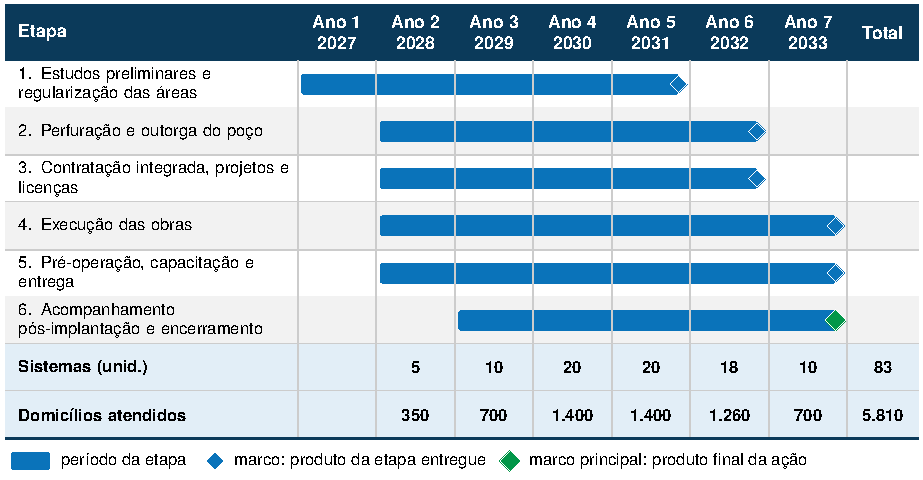
\includegraphics[width=15.64cm]{figuras/g-crono-3223.pdf}
  \fonteMOP{Fonte: IAT (2026), com quantidades da planilha PSH\_CUSTO\_Consolidada (PARANÁ, 2026).}
  % Texto alternativo: Cronograma anual de 2027 a 2033 com as etapas e as quantidades a entregar da implantação dos sistemas coletivos de abastecimento de água.
\end{figure}

\phantomsection
\addcontentsline{toc}{subsection}{9. Interfaces e dependências}
\subsection*{9. Interfaces e dependências}

A ação depende da entidade gestora pactuada, do diagnóstico das comunidades, da supervisão das obras e dos instrumentos de gestão de recursos hídricos do Programa, como a outorga, o SIGARH e os dados de águas subterrâneas. Fornece ao esgotamento sanitário as comunidades atendidas com água, aos modelos de gestão os sistemas concluídos para entrega e à UGP o número de pessoas atendidas para o indicador do componente (Figura~\ref{interf-3223}).

\begin{figure}[H]
  \centering
  \caption{Interfaces e dependências da implantação dos sistemas coletivos de abastecimento de água}\label{interf-3223}
  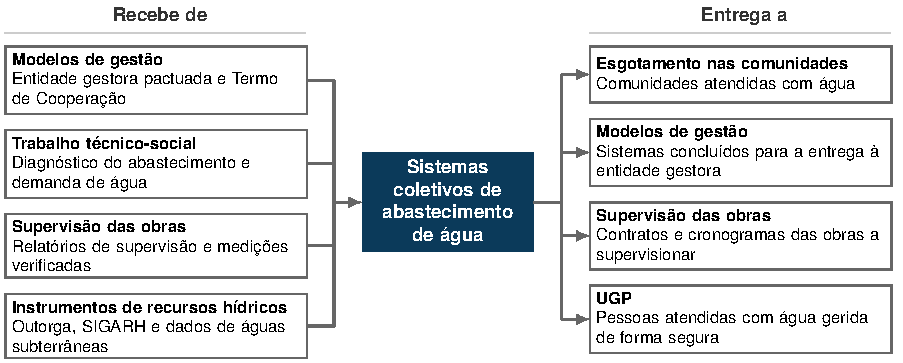
\includegraphics[width=15.30cm]{figuras/g-interf-3223.pdf}
  \fonteMOP{Fonte: IAT (2026).}
  % Texto alternativo: Diagrama das interfaces da implantação dos sistemas coletivos de abastecimento de água: insumos recebidos de outras partes do Programa e produtos entregues a elas.
\end{figure}

\phantomsection
\addcontentsline{toc}{subsection}{10. Documentos complementares}
\subsection*{10. Documentos complementares}

\begin{itemize}
  \item Termo de Referência e edital da contratação integrada de projetos e obras (a elaborar);
  \item Plano de Operação e Manutenção dos sistemas (a elaborar);
  \item Portaria GM/MS nº~888/2021, que altera o Anexo XX da Portaria de Consolidação GM/MS nº~5/2017 (padrão de potabilidade da água para consumo humano);
  \item Normas da Associação Brasileira de Normas Técnicas (ABNT) NBR 12212:2017 e NBR 12244:2006 (projeto e construção de poço tubular) e demais normas ABNT de projeto de sistemas de abastecimento de água;
  \item Lei nº~9.433/1997 e Lei Estadual nº~12.726/1999 (outorga de direito de uso de recursos hídricos) e normas de licenciamento ambiental do IAT;
  \item Caderno AQ e Caderno AS;
  \item Notas técnicas de origem (IAT, 2026a; IAT, 2026b).
\end{itemize}

\acao{Ação 3.2.2.4 – Programa Sanepar Rural}

\phantomsection
\addcontentsline{toc}{subsection}{1. Contextualização}
\subsection*{1. Contextualização}

A ação implanta 222 sistemas coletivos de abastecimento de água em comunidades rurais de municípios com Contrato de Concessão ou de Programa vigente com a Sanepar, entre 2027 e 2031. A Sanepar elabora os estudos e os projetos, presta apoio técnico, ambiental e socioeconômico às comunidades e fornece capacitação, materiais hidráulicos e equipamentos; o município executa as obras; e a comunidade constitui a associação de moradores responsável pela operação do sistema (IAT, 2026b; SANEPAR, [s.d.]).

Mesmo nos municípios atendidos pela Sanepar, as comunidades rurais situam-se fora do alcance das redes urbanas e dependem de nascentes e poços rasos, sujeitos à contaminação e às estiagens. O Programa Sanepar Rural implanta nessas comunidades sistemas coletivos com água tratada, com base na capacidade técnica da companhia e na estrutura de gestão local das associações.

A ação responde pela maior parcela do indicador de pessoas atendidas com água gerida de forma segura: cerca de 43,5 mil das 59.780 pessoas previstas. Constitui também a contrapartida do Estado na atividade, no valor de R\$~67,15 milhões (cerca de US\$~12,3 milhões, à taxa de câmbio de R\$~5,46 adotada no Documento de Avaliação do Projeto – PAD), aplicados com recursos próprios da Sanepar (PARANÁ, 2026).

\textbf{Inclui:} o levantamento técnico e o estudo de engenharia; o Termo de Compromisso e Responsabilidade vinculado ao Contrato de Concessão ou de Programa; os projetos de engenharia dos sistemas; o fornecimento de materiais hidráulicos e o apoio técnico às obras municipais; a mobilização e a organização comunitária; a capacitação e a educação ambiental; e o monitoramento e o suporte pós-obra.

\textbf{Não inclui:} os sistemas implantados pelo IAT nem recursos do empréstimo do BIRD.

\textbf{Valor previsto:} R\$~67,15 milhões (empréstimo BIRD: R\$~0,00 milhões; contrapartida: R\$~67,15 milhões), conforme a planilha PSH\_CUSTO\_Consolidada.

\phantomsection
\addcontentsline{toc}{subsection}{2. Área de atuação}
\subsection*{2. Área de atuação}

A ação abrange os municípios com Contrato de Concessão ou de Programa vigente com a Sanepar, em todo o Estado. As comunidades atendidas são selecionadas pelos critérios do manual do Programa Sanepar Rural, com base na demanda das comunidades e dos municípios e na viabilidade técnica do sistema.

\pendencia{O Acordo de Empréstimo, item (j)(vii) das definições, exige a identificação das áreas rurais da Parte 3.2. Solicitar à Sanepar a lista dos municípios e das comunidades atendidas, com os critérios de priorização do manual do programa.}

\phantomsection
\addcontentsline{toc}{subsection}{3. Arranjo institucional e partes interessadas}
\subsection*{3. Arranjo institucional e partes interessadas}

A Sanepar é a executora da ação, com estrutura técnica e recursos de contrapartida próprios. Os municípios celebram o Termo de Compromisso e Responsabilidade e executam as obras, e as comunidades constituem as associações de moradores e participam da capacitação. O IAT acompanha a compatibilização com o modelo de gestão e com a outorga de direito de uso de recursos hídricos, e a UGP consolida a comprovação da contrapartida e o reporte ao Banco Mundial.

\pendencia{Indicar a diretoria e a gerência da Sanepar responsáveis pelo Programa Sanepar Rural.}

\begin{itemize}
  \item \textbf{Executora:} Sanepar;
  \item \textbf{Intervenientes:} municípios; IAT (modelo de gestão e outorga); UGP;
  \item \textbf{Público envolvido:} comunidades rurais e associações de moradores.
\end{itemize}

Os beneficiários diretos são os moradores das comunidades atendidas pelos 222 sistemas, cerca de 43,5 mil pessoas. Os beneficiários indiretos são os municípios e os serviços de saúde, com a redução das doenças de veiculação hídrica.

\phantomsection
\addcontentsline{toc}{subsection}{4. Processo de execução operacional}
\subsection*{4. Processo de execução operacional}

As atividades observam o manual do Programa Sanepar Rural e compreendem seis etapas (Figura~\ref{raias-3224}). Em cada comunidade, a Sanepar executa o levantamento técnico e o projeto, formaliza a parceria com o município e fornece os materiais; o município executa a obra com apoio técnico da companhia; e a comunidade constitui a associação e participa da capacitação. Concluída a obra, a Sanepar monitora a qualidade da água e presta suporte às associações.

\begin{figure}[H]
  \centering
  \caption{Fluxograma do Programa Sanepar Rural: entradas, etapas por responsável e saídas}\label{raias-3224}
  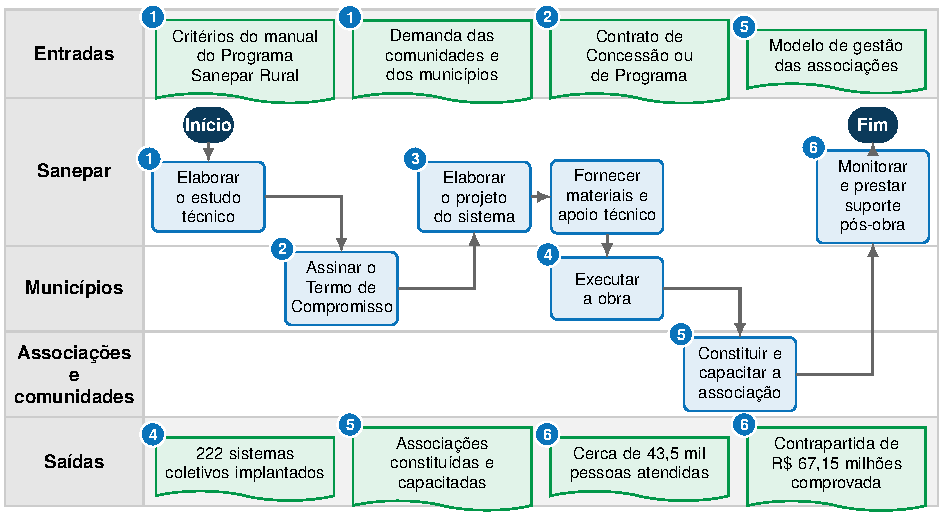
\includegraphics[width=15.96cm]{figuras/g-raias-3224.pdf}
  \fonteMOP{Fonte: IAT (2026), com base em IAT (2026b) e SANEPAR ([s.d.]).}
  % Texto alternativo: Fluxograma em raias da Sanepar, dos municípios e das associações, do estudo técnico ao suporte pós-obra, com as entradas no topo e as saídas na base.
\end{figure}

\phantomsection
\subsubsection*{4.1 Etapa 1: Levantamento técnico e estudo de engenharia}

\textbf{Atividades:} levantamento das condições da comunidade e estudo técnico de engenharia do sistema.

\textbf{Entradas:} demanda da comunidade e do município; critérios do manual do programa.

\textbf{Responsáveis:} Sanepar (executa e aprova); município (consultado).

\textbf{Produto:} estudo técnico da comunidade.

\phantomsection
\subsubsection*{4.2 Etapa 2: Termo de Compromisso com o município}

\textbf{Atividades:} formalização da parceria por Termo de Compromisso e Responsabilidade vinculado ao Contrato de Concessão ou de Programa, com as obrigações de cada parte.

\textbf{Entradas:} estudo técnico; Contrato de Concessão ou de Programa vigente.

\textbf{Responsáveis:} Sanepar e município (executam); Sanepar (aprova).

\textbf{Produto:} Termo de Compromisso e Responsabilidade assinado.

\phantomsection
\subsubsection*{4.3 Etapa 3: Projetos de engenharia}

\textbf{Atividades:} elaboração do projeto de engenharia do sistema de abastecimento de água.

\textbf{Entradas:} estudo técnico; Termo de Compromisso.

\textbf{Responsáveis:} Sanepar (executa e aprova); município (informado).

\textbf{Produto:} projeto do sistema.

\phantomsection
\subsubsection*{4.4 Etapa 4: Execução das obras com apoio da Sanepar}

\textbf{Atividades:} fornecimento dos materiais hidráulicos pela Sanepar; execução das obras pelo município, diretamente ou por contratação própria, com apoio técnico da companhia.

\textbf{Entradas:} projeto aprovado; materiais; outorga e licenças, quando exigidas.

\textbf{Responsáveis:} município (executa a obra); Sanepar (fornece os materiais, presta apoio técnico e aprova a obra).

\textbf{Produto:} sistema implantado.

\phantomsection
\subsubsection*{4.5 Etapa 5: Organização comunitária e capacitação}

\textbf{Atividades:} apoio à constituição da associação de moradores; capacitação em uso racional da água, higiene e manutenção preventiva; educação ambiental.

\textbf{Entradas:} comunidade mobilizada; modelo de gestão.

\textbf{Responsáveis:} Sanepar (executa e aprova); comunidade (executa); IAT (consultado quanto ao modelo de gestão).

\textbf{Produto:} associação constituída e capacitada.

\phantomsection
\subsubsection*{4.6 Etapa 6: Monitoramento e suporte pós-obra}

\textbf{Atividades:} monitoramento pós-obra da qualidade da água e suporte operacional às associações; relatório técnico de cada sistema; reporte anual à UGP dos sistemas implantados, das pessoas atendidas e dos valores aplicados.

\textbf{Entradas:} sistema implantado; associação constituída.

\textbf{Responsáveis:} Sanepar (executa e aprova o relatório técnico); UGP (informada).

\textbf{Produto:} relatório técnico aprovado.

\phantomsection
\subsubsection*{4.7 Modalidade de execução}

O item de custo é o de sistemas coletivos de abastecimento de água com recursos de contrapartida: 222 sistemas ao custo médio de R\$~302.464,42, no total de R\$~67,15 milhões, integralmente com recursos próprios da Sanepar. A execução ocorre por convênio, formalizado em Termo de Compromisso e Responsabilidade entre a Sanepar e cada município, conforme o manual do programa.

As aquisições da Sanepar observam o Regulamento de Licitações e Contratos da companhia, e as obras contratadas pelos municípios, a legislação de licitações aplicável. A Sanepar comprova à UGP os valores aplicados e os sistemas implantados, para registro da contrapartida.

\pendencia{Confirmar com a UGP e o Banco Mundial se as aquisições e as obras financiadas com contrapartida seguem as regras da Sanepar e dos municípios e quais requisitos do Programa se aplicam.}

\phantomsection
\addcontentsline{toc}{subsection}{5. Matriz de responsabilidades}
\subsection*{5. Matriz de responsabilidades}

O Quadro~\ref{raci-3224} apresenta o papel de cada parte em cada etapa.

\begin{quadro}[H]
  \caption{Matriz de responsabilidades do Programa Sanepar Rural}\label{raci-3224}
  \footnotesize\renewcommand{\arraystretch}{1.25}\setlength{\tabcolsep}{3pt}
  \begin{tabular}{>{\raggedright\arraybackslash}p{\dimexpr 0.2536\linewidth-2\tabcolsep\relax}>{\centering\arraybackslash}p{\dimexpr 0.0882\linewidth-2\tabcolsep\relax}>{\centering\arraybackslash}p{\dimexpr 0.0882\linewidth-2\tabcolsep\relax}>{\centering\arraybackslash}p{\dimexpr 0.0882\linewidth-2\tabcolsep\relax}>{\centering\arraybackslash}p{\dimexpr 0.0882\linewidth-2\tabcolsep\relax}>{\centering\arraybackslash}p{\dimexpr 0.0882\linewidth-2\tabcolsep\relax}>{\centering\arraybackslash}p{\dimexpr 0.0882\linewidth-2\tabcolsep\relax}>{\centering\arraybackslash}p{\dimexpr 0.2173\linewidth-2\tabcolsep\relax}}
    \rowcolor{azulEscuro}\textcolor{white}{\textbf{Parte}} & \textcolor{white}{\textbf{E1}} & \textcolor{white}{\textbf{E2}} & \textcolor{white}{\textbf{E3}} & \textcolor{white}{\textbf{E4}} & \textcolor{white}{\textbf{E5}} & \textcolor{white}{\textbf{E6}} & \textcolor{white}{\textbf{Produto final}} \\
    Sanepar & \raci{R} \raci{A} & \raci{R} \raci{A} & \raci{R} \raci{A} & \raci{A} & \raci{R} \raci{A} & \raci{R} \raci{A} & \raci{R} \raci{A} \\ \arrayrulecolor{cinza20}\hline
    \rowcolor{cinza5}Municípios & \raci{C} & \raci{R} & \raci{I} & \raci{R} & \raci{C} & \raci{I} & \raci{I} \\ \arrayrulecolor{cinza20}\hline
    Comunidades e associações & \raci{C} & – & – & \raci{I} & \raci{R} & \raci{C} & \raci{R} \\ \arrayrulecolor{cinza20}\hline
    \rowcolor{cinza5}IAT & – & – & – & – & \raci{C} & \raci{I} & \raci{I} \\ \arrayrulecolor{cinza20}\hline
    UGP & – & – & – & – & – & \raci{I} & \raci{I} \\ \noalign{\global\arrayrulewidth=1pt}\arrayrulecolor{azulEscuro}\hline\noalign{\global\arrayrulewidth=0.4pt}
  \end{tabular}
  \fonteMOP{Fonte: IAT (2026).}
  \notaMOP{Nota: E1 a E6 correspondem às Etapas 1 a 6 do item 4. \raci{R} executa (pode haver mais de um); \raci{A} aprova ou valida o produto (um por etapa); \raci{C} é consultado previamente; \raci{I} é informado posteriormente. Produto final: sistemas implantados e pessoas atendidas.}
\end{quadro}

\phantomsection
\addcontentsline{toc}{subsection}{6. Metas, indicadores e comprovação}
\subsection*{6. Metas, indicadores e comprovação}

A meta é a implantação de 222 sistemas de 2027 a 2031 (Quadro~\ref{metas-3224}).

\begin{quadro}[H]
  \caption{Metas anuais do Programa Sanepar Rural}\label{metas-3224}
  \footnotesize\renewcommand{\arraystretch}{1.25}\setlength{\tabcolsep}{3pt}
  \begin{tabular}{>{\raggedright\arraybackslash}p{\dimexpr 0.2095\linewidth-2\tabcolsep\relax}>{\raggedright\arraybackslash}p{\dimexpr 0.1268\linewidth-2\tabcolsep\relax}>{\raggedleft\arraybackslash}p{\dimexpr 0.0794\linewidth-2\tabcolsep\relax}>{\raggedleft\arraybackslash}p{\dimexpr 0.0794\linewidth-2\tabcolsep\relax}>{\raggedleft\arraybackslash}p{\dimexpr 0.0794\linewidth-2\tabcolsep\relax}>{\raggedleft\arraybackslash}p{\dimexpr 0.0794\linewidth-2\tabcolsep\relax}>{\raggedleft\arraybackslash}p{\dimexpr 0.0794\linewidth-2\tabcolsep\relax}>{\raggedleft\arraybackslash}p{\dimexpr 0.0794\linewidth-2\tabcolsep\relax}>{\raggedleft\arraybackslash}p{\dimexpr 0.0794\linewidth-2\tabcolsep\relax}>{\raggedleft\arraybackslash}p{\dimexpr 0.1081\linewidth-2\tabcolsep\relax}}
    \rowcolor{azulEscuro}\textcolor{white}{\textbf{Produto}} & \textcolor{white}{\textbf{Unidade}} & \centering\arraybackslash \textcolor{white}{\textbf{Ano 1}} & \centering\arraybackslash \textcolor{white}{\textbf{Ano 2}} & \centering\arraybackslash \textcolor{white}{\textbf{Ano 3}} & \centering\arraybackslash \textcolor{white}{\textbf{Ano 4}} & \centering\arraybackslash \textcolor{white}{\textbf{Ano 5}} & \centering\arraybackslash \textcolor{white}{\textbf{Ano 6}} & \centering\arraybackslash \textcolor{white}{\textbf{Ano 7}} & \centering\arraybackslash \textcolor{white}{\textbf{Total}} \\
    Sistemas coletivos de abastecimento de água & sistemas & 45 & 41 & 42 & 43 & 51 & – & – & 222 \\ \arrayrulecolor{cinza20}\hline
    \rowcolor{cinza5}Pessoas atendidas & pessoas & 8.820 & 8.036 & 8.232 & 8.428 & 9.996 & – & – & 43.512 \\ \noalign{\global\arrayrulewidth=1pt}\arrayrulecolor{azulEscuro}\hline\noalign{\global\arrayrulewidth=0.4pt}
  \end{tabular}
  \fonteMOP{Fonte: Planilha PSH\_CUSTO\_Consolidada, versão v2408 (PARANÁ, 2026).}
  \notaMOP{Nota: Ano 1 = 2027 e Ano 7 = 2033. Pessoas estimadas com 70 domicílios por sistema e 2,8 pessoas por domicílio, conforme o indicador do componente.}
\end{quadro}

Os indicadores constam do Quadro~\ref{ind-3224}. A Sanepar informa anualmente à UGP os sistemas implantados, as pessoas atendidas, com desagregação por sexo e para jovens de 15 a 24 anos, e os valores de contrapartida aplicados.

\begin{quadro}[H]
  \caption{Indicadores do Programa Sanepar Rural}\label{ind-3224}
  \footnotesize\renewcommand{\arraystretch}{1.25}\setlength{\tabcolsep}{3pt}
  \begin{tabular}{>{\raggedright\arraybackslash}p{\dimexpr 0.3165\linewidth-2\tabcolsep\relax}>{\raggedright\arraybackslash}p{\dimexpr 0.1378\linewidth-2\tabcolsep\relax}>{\raggedleft\arraybackslash}p{\dimexpr 0.1102\linewidth-2\tabcolsep\relax}>{\raggedleft\arraybackslash}p{\dimexpr 0.1599\linewidth-2\tabcolsep\relax}>{\raggedright\arraybackslash}p{\dimexpr 0.2756\linewidth-2\tabcolsep\relax}}
    \rowcolor{azulEscuro}\textcolor{white}{\textbf{Indicador}} & \textcolor{white}{\textbf{Unidade}} & \centering\arraybackslash \textcolor{white}{\textbf{Linha de base (2025)}} & \centering\arraybackslash \textcolor{white}{\textbf{Meta}} & \textcolor{white}{\textbf{Frequência e fonte dos dados}} \\
    Sistemas implantados pelo Programa Sanepar Rural & sistemas & 0 & 222 & Anual; Sanepar \\ \arrayrulecolor{cinza20}\hline
    \rowcolor{cinza5}Pessoas atendidas com água gerida de forma segura (parcela do indicador do componente) & pessoas & 0 & 43.500 & Anual; Sanepar, com desagregação por sexo e jovens \\ \arrayrulecolor{cinza20}\hline
    Contrapartida aplicada & R\$~milhões & 0 & 67,15 & Anual; Sanepar e UGP \\ \noalign{\global\arrayrulewidth=1pt}\arrayrulecolor{azulEscuro}\hline\noalign{\global\arrayrulewidth=0.4pt}
  \end{tabular}
  \fonteMOP{Fonte: IAT (2026).}
\end{quadro}

\pendencia{O MOP de março atribuía ao Programa Sanepar Rural a meta total do indicador (59.780 pessoas), que inclui os sistemas do IAT. A parcela da Sanepar é de cerca de 43.500 pessoas. Confirmar com a Sanepar e citar o manual do programa com título, versão e data.}

Os critérios de aceite e as evidências de cada produto constam do Quadro~\ref{aceite-3224}. A evidência de conclusão de cada sistema é o relatório técnico aprovado pela Sanepar.

\begin{quadro}[H]
  \caption{Critérios de aceite e evidências do Programa Sanepar Rural}\label{aceite-3224}
  \footnotesize\renewcommand{\arraystretch}{1.25}\setlength{\tabcolsep}{5pt}
  \begin{tabular}{>{\raggedright\arraybackslash}p{\dimexpr 0.2150\linewidth-2\tabcolsep\relax}>{\raggedright\arraybackslash}p{\dimexpr 0.3386\linewidth-2\tabcolsep\relax}>{\raggedright\arraybackslash}p{\dimexpr 0.2921\linewidth-2\tabcolsep\relax}>{\raggedright\arraybackslash}p{\dimexpr 0.1543\linewidth-2\tabcolsep\relax}}
    \rowcolor{azulEscuro}\textcolor{white}{\textbf{Produto}} & \textcolor{white}{\textbf{Critério de aceite}} & \textcolor{white}{\textbf{Evidência de comprovação}} & \textcolor{white}{\textbf{Responsável pela validação}} \\
    Termo de Compromisso & Assinado pela Sanepar e pelo município & Termo assinado & Sanepar \\ \arrayrulecolor{cinza20}\hline
    \rowcolor{cinza5}Projeto do sistema & Aprovado conforme as normas da Sanepar & Projeto aprovado & Sanepar \\ \arrayrulecolor{cinza20}\hline
    Sistema implantado & Obra concluída e em operação, com água conforme o padrão de potabilidade & Relatório técnico aprovado; laudos de qualidade da água & Sanepar \\ \arrayrulecolor{cinza20}\hline
    \rowcolor{cinza5}Associação capacitada & Associação constituída e capacitada em operação e manutenção & Registro da associação; listas de presença & Sanepar \\ \arrayrulecolor{cinza20}\hline
    Contrapartida comprovada & Valores aplicados registrados por sistema & Relatório financeiro da Sanepar & UGP \\ \noalign{\global\arrayrulewidth=1pt}\arrayrulecolor{azulEscuro}\hline\noalign{\global\arrayrulewidth=0.4pt}
  \end{tabular}
  \fonteMOP{Fonte: IAT (2026).}
\end{quadro}

\phantomsection
\addcontentsline{toc}{subsection}{7. Gestão de riscos e impactos ambientais e sociais}
\subsection*{7. Gestão de riscos e impactos ambientais e sociais}

Os riscos são análogos aos dos sistemas implantados pelo IAT: impactos temporários das obras, segurança dos trabalhadores e da comunidade, uso das áreas das estruturas, qualidade da água e participação das comunidades. Por integrar o Programa, a ação observa os instrumentos do Caderno AS (Quadro~\ref{nas-3224}).

\begin{quadro}[H]
  \caption{Aplicação das Normas Ambientais e Sociais ao Programa Sanepar Rural}\label{nas-3224}
  \footnotesize\renewcommand{\arraystretch}{1.25}\setlength{\tabcolsep}{5pt}
  \begin{tabular}{>{\raggedright\arraybackslash}p{\dimexpr 0.1874\linewidth-2\tabcolsep\relax}>{\raggedright\arraybackslash}p{\dimexpr 0.3716\linewidth-2\tabcolsep\relax}>{\raggedright\arraybackslash}p{\dimexpr 0.4410\linewidth-2\tabcolsep\relax}}
    \rowcolor{azulEscuro}\textcolor{white}{\textbf{NAS}} & \textcolor{white}{\textbf{Aplicação à ação}} & \textcolor{white}{\textbf{Medidas e instrumentos}} \\
    NAS 1 – Avaliação e gestão de riscos & Obras em cada comunidade & Triagem socioambiental; licenças, quando exigidas; procedimentos ambientais da Sanepar \\ \arrayrulecolor{cinza20}\hline
    \rowcolor{cinza5}NAS 2 – Condições de trabalho & Trabalhadores das obras municipais e da Sanepar & Uso de EPI e protocolos de saúde e segurança do trabalho \\ \arrayrulecolor{cinza20}\hline
    NAS 3 – Eficiência de recursos e prevenção da poluição & Captação de água e resíduos de obra & Outorga; controle de perdas; destinação adequada dos resíduos \\ \arrayrulecolor{cinza20}\hline
    \rowcolor{cinza5}NAS 4 – Saúde e segurança da comunidade & Valas, trânsito de máquinas e qualidade da água & Sinalização das obras; monitoramento da qualidade da água pela Sanepar \\ \arrayrulecolor{cinza20}\hline
    NAS 5 – Aquisição de terras & Áreas para captação e reservação & Verificação da titularidade e anuência; ausência de reassentamento involuntário \\ \arrayrulecolor{cinza20}\hline
    \rowcolor{cinza5}NAS 10 – Engajamento das partes interessadas & Comunidades e associações & Mobilização e organização comunitária; canal de atendimento da Sanepar e Mecanismo de Queixas e Reclamações do Programa \\ \noalign{\global\arrayrulewidth=1pt}\arrayrulecolor{azulEscuro}\hline\noalign{\global\arrayrulewidth=0.4pt}
  \end{tabular}
  \fonteMOP{Fonte: IAT (2026), com base nos instrumentos do Caderno AS.}
  \notaMOP{Nota: as NAS 6, 7 e 8 são verificadas na triagem de cada sistema.}
\end{quadro}

\pendencia{Confirmar com a UGP quais instrumentos do Caderno AS se aplicam às ações executadas com recursos de contrapartida.}

\phantomsection
\addcontentsline{toc}{subsection}{8. Cronograma}
\subsection*{8. Cronograma}

A ação ocorre de 2027 a 2031 (Figura~\ref{crono-3224}): 45 sistemas em 2027, 41 em 2028, 42 em 2029, 43 em 2030 e 51 em 2031. Os estudos, os termos e os projetos de cada ano antecedem as obras do ano seguinte, e o suporte pós-obra prossegue como atividade de rotina da Sanepar após 2031.

\begin{figure}[H]
  \centering
  \caption{Cronograma das etapas e das entregas do Programa Sanepar Rural}\label{crono-3224}
  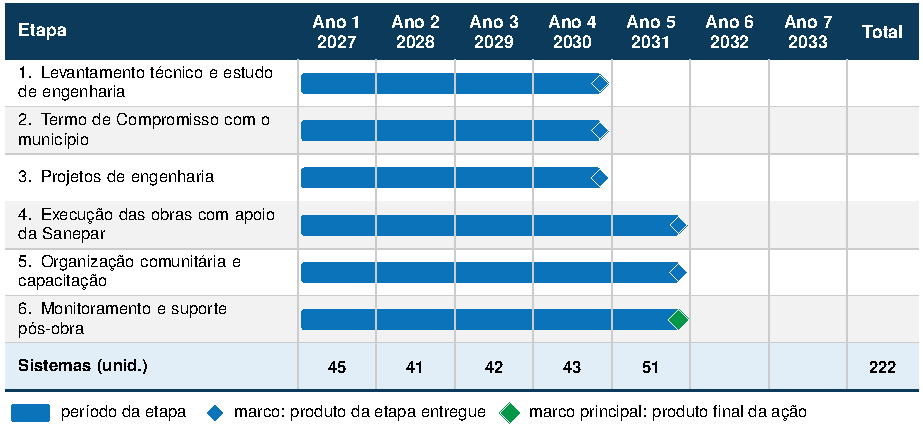
\includegraphics[width=15.64cm]{figuras/g-crono-3224.pdf}
  \fonteMOP{Fonte: IAT (2026), com quantidades da planilha PSH\_CUSTO\_Consolidada (PARANÁ, 2026).}
  % Texto alternativo: Cronograma anual de 2027 a 2033 com as etapas e as quantidades a entregar do Programa Sanepar Rural.
\end{figure}

\phantomsection
\addcontentsline{toc}{subsection}{9. Interfaces e dependências}
\subsection*{9. Interfaces e dependências}

A ação recebe dos modelos de gestão o arranjo aplicável às associações de moradores e da política estadual de saneamento rural as diretrizes setoriais. Fornece à UGP o número de pessoas atendidas e a comprovação da contrapartida e alimenta o indicador de pessoas atendidas com água gerida de forma segura (Figura~\ref{interf-3224}).

\begin{figure}[H]
  \centering
  \caption{Interfaces e dependências do Programa Sanepar Rural}\label{interf-3224}
  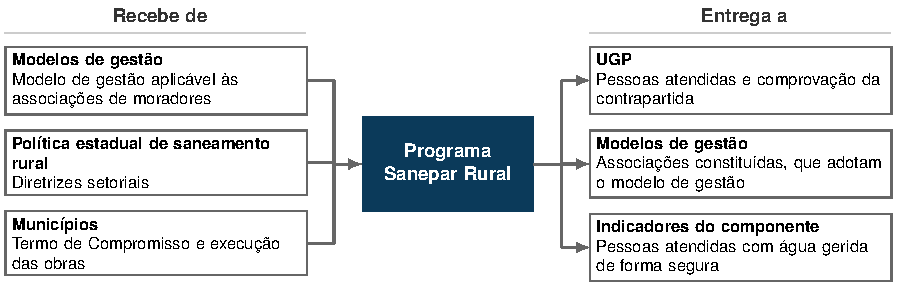
\includegraphics[width=15.30cm]{figuras/g-interf-3224.pdf}
  \fonteMOP{Fonte: IAT (2026).}
  % Texto alternativo: Diagrama das interfaces do Programa Sanepar Rural: insumos recebidos de outras partes do Programa e produtos entregues a elas.
\end{figure}

\phantomsection
\addcontentsline{toc}{subsection}{10. Documentos complementares}
\subsection*{10. Documentos complementares}

\begin{itemize}
  \item Manual do Programa Sanepar Rural (SANEPAR, [s.d.]);
  \item Contratos de Concessão e de Programa entre a Sanepar e os municípios;
  \item Modelo do Termo de Compromisso e Responsabilidade;
  \item Regulamento de Licitações e Contratos da Sanepar;
  \item Portaria GM/MS nº~888/2021 (padrão de potabilidade);
  \item Caderno AS.
\end{itemize}

\acao{Ação 3.2.2.5 – Esgotamento sanitário nas comunidades atendidas com água}

\phantomsection
\addcontentsline{toc}{subsection}{1. Contextualização}
\subsection*{1. Contextualização}

A ação implanta soluções individuais de esgotamento sanitário em 4.067 domicílios das comunidades atendidas pelos sistemas coletivos de abastecimento de água do IAT, entre 2028 e 2033. Trata-se de sistemas descentralizados, implantados em cada domicílio, que coletam, tratam e promovem a disposição final ou o reúso do esgoto próximo ao ponto de geração, solução adequada à baixa densidade de ocupação do meio rural (IAT, 2026a).

No meio rural do Paraná, apenas 1,46\% dos moradores declaram ligação à rede geral ou pluvial, segundo o Censo 2022, e o Sistema Nacional de Informações em Saneamento Básico (Sinisa) indica que cerca de 3,9\% da população rural é atendida por rede coletora (IAT, 2026a). O esgoto lançado sem tratamento no solo e nos corpos hídricos aporta matéria orgânica, nutrientes e microrganismos patogênicos aos mananciais superficiais e subterrâneos utilizados para abastecimento. Como a ampliação do abastecimento de água eleva o volume de esgoto gerado, as soluções de esgotamento sanitário acompanham a implantação dos sistemas de abastecimento, de modo a evitar a contaminação da própria fonte de abastecimento da comunidade.

As soluções observam a ABNT NBR 17076:2024, que substituiu as normas ABNT NBR 7229:1993 e NBR 13969:1997 e estabelece alternativas de tratamento local para vazões de até 12.000 L/dia e carga orgânica de até 3,80 kg de demanda bioquímica de oxigênio (DBO) por dia (ABNT, 2024). O desempenho dessas soluções depende da simplicidade de construção e de operação, uma vez que mesmo tecnologias adequadas apresentam falhas quando mal executadas ou mal operadas. Por esse motivo, a seleção privilegia soluções de baixa complexidade, compatíveis com as condições de cada domicílio (TONETTI et al., 2018), e contempla o manejo e a destinação adequada do lodo.

A Figura~\ref{esquema-esgoto} apresenta um exemplo de arranjo.

\begin{figure}[H]
  \centering
  \caption{Exemplo de solução individual de esgotamento sanitário}\label{esquema-esgoto}
  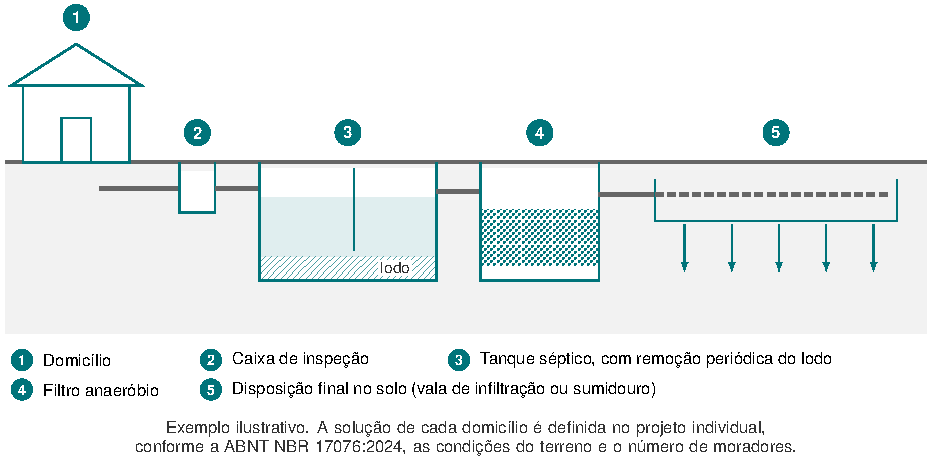
\includegraphics[width=15.78cm]{figuras/f-esquema-esgoto.pdf}
  \fonteMOP{Fonte: IAT (2026), com base em ABNT (2024) e Tonetti et al. (2018). Esquema ilustrativo, sem escala.}
  % Texto alternativo: Esquema em corte com domicílio, caixa de inspeção, tanque séptico, filtro anaeróbio e vala de infiltração.
\end{figure}

A ação contribui para o indicador de pessoas atendidas com, pelo menos, esgotamento sanitário, com cerca de 11,4 mil das 17.800 pessoas previstas; as demais decorrem do esgotamento sanitário em mananciais.

\textbf{Inclui:} a contratação das soluções e das obras civis; o projeto individual de cada domicílio; a instalação conforme a ABNT NBR 17076:2024; a verificação técnica; a orientação do proprietário quanto ao uso e à manutenção; a medição, a comprovação e o pagamento; e a substituição de soluções inadequadas.

\textbf{Não inclui:} redes coletoras nem intervenções no interior das moradias. A manutenção após a entrega, inclusive a limpeza periódica, cabe ao proprietário, conforme a orientação recebida.

\pendencia{Definir o responsável pela coleta e pela destinação do lodo das soluções individuais após a entrega (proprietário, associação, município ou serviço contratado).}

\textbf{Valor previsto:} R\$~32,54 milhões (empréstimo BIRD: R\$~32,54 milhões; contrapartida: R\$~0,00 milhões), conforme a planilha PSH\_CUSTO\_Consolidada.

\phantomsection
\addcontentsline{toc}{subsection}{2. Área de atuação}
\subsection*{2. Área de atuação}

A ação abrange as 83 comunidades atendidas pelos sistemas coletivos de abastecimento de água (Figura~\ref{mapa}). O número de domicílios foi estimado com os dados do Censo 2022 por setor censitário e do CNEFE: dos 5.810 domicílios dessas comunidades, 4.067 (70\%) não dispõem de esgotamento sanitário adequado (IAT, 2026a). Os domicílios atendidos são confirmados individualmente pelo diagnóstico do trabalho técnico-social.

\phantomsection
\addcontentsline{toc}{subsection}{3. Arranjo institucional e partes interessadas}
\subsection*{3. Arranjo institucional e partes interessadas}

O IAT, por meio da DISAR, contrata a empresa, fiscaliza a instalação, valida as medições e efetua o pagamento. A empresa contratada elabora o projeto de cada domicílio e executa a instalação, e o proprietário autoriza a intervenção, acompanha a obra e confirma a execução. A supervisora das obras apoia a fiscalização, e a UGP acompanha a execução.

\begin{itemize}
  \item \textbf{Intervenientes:} empresa contratada; empresa supervisora das obras; prefeituras, no apoio à articulação local;
  \item \textbf{Público envolvido:} proprietários e moradores dos domicílios atendidos.
\end{itemize}

Os beneficiários diretos são os moradores dos 4.067 domicílios sem esgotamento sanitário adequado, cerca de 11,4 mil pessoas. Os beneficiários indiretos são os demais moradores das comunidades e das bacias, em razão da redução da carga de esgoto lançada no solo e nos corpos hídricos.

\phantomsection
\addcontentsline{toc}{subsection}{4. Processo de execução operacional}
\subsection*{4. Processo de execução operacional}

A partir do diagnóstico de cada domicílio, a ação compreende sete etapas (Figura~\ref{raias-3225}). O proprietário participa em dois momentos: autoriza a intervenção na Etapa 1 e confirma a execução na Etapa 6. A evidência de conclusão de cada lote é o relatório técnico aprovado, acompanhado do comprovante de pagamento.

\begin{figure}[H]
  \centering
  \caption{Fluxograma do esgotamento sanitário nas comunidades: entradas, etapas por responsável e saídas}\label{raias-3225}
  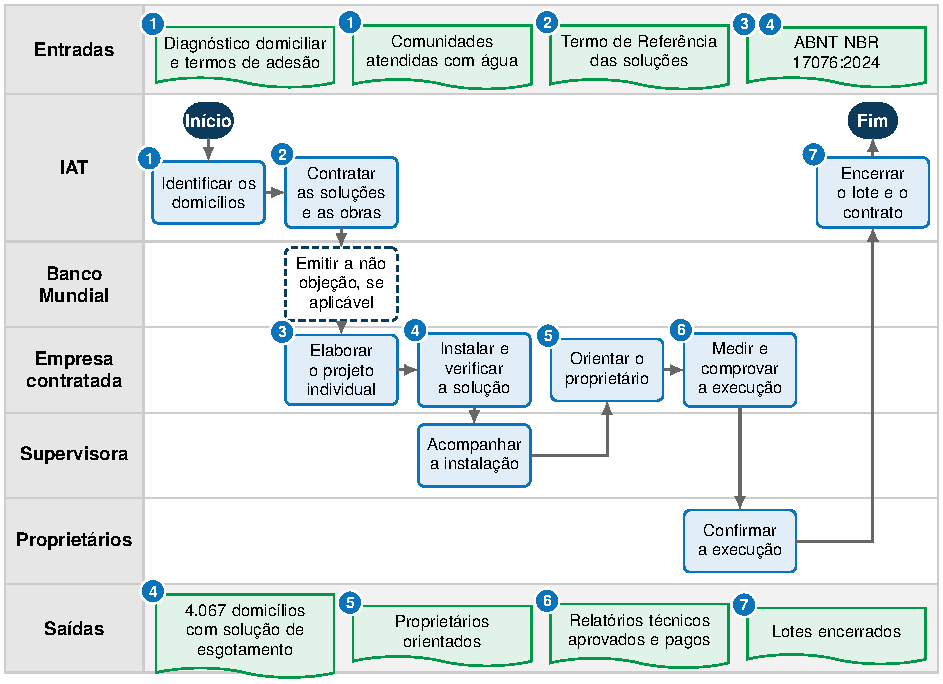
\includegraphics[width=15.96cm]{figuras/g-raias-3225.pdf}
  \fonteMOP{Fonte: IAT (2026).}
  % Texto alternativo: Fluxograma em raias do esgotamento sanitário nas comunidades, com uma raia por instituição, as etapas numeradas na raia do executor, as entradas no topo e as saídas na base.
\end{figure}

\phantomsection
\subsubsection*{4.1 Etapa 1: Identificação dos domicílios}

\textbf{Atividades:} seleção, com base no diagnóstico do trabalho técnico-social, dos domicílios sem esgotamento sanitário adequado; confirmação da adesão e da autorização do proprietário para a intervenção.

\textbf{Entradas:} diagnóstico domiciliar e termos de adesão (trabalho técnico-social).

\textbf{Responsáveis:} IAT (executa e aprova); proprietários (consultados).

\textbf{Produto:} lista de domicílios por comunidade.

\phantomsection
\subsubsection*{4.2 Etapa 2: Contratação das soluções e das obras}

\textbf{Atividades:} elaboração e aprovação do Termo de Referência das soluções descentralizadas e das obras civis de instalação; publicação do edital; licitação; contratação das empresas.

\textbf{Entradas:} lista de domicílios; especificações conforme a ABNT NBR 17076:2024.

\textbf{Responsáveis:} IAT (executa e aprova); UGP e Banco Mundial (consultados, quando houver revisão prévia).

\textbf{Produto:} contrato assinado.

\phantomsection
\subsubsection*{4.3 Etapa 3: Projeto individual por domicílio}

\textbf{Atividades:} elaboração, pela empresa contratada, do projeto de cada domicílio, considerada a topografia do terreno, o número de moradores, a capacidade de infiltração do solo e a solução de tratamento adequada, inclusive o manejo do lodo.

\textbf{Entradas:} contrato; dados do diagnóstico domiciliar.

\textbf{Responsáveis:} empresa contratada (executa); IAT (aprova); proprietário (consultado).

\textbf{Produto:} projeto aprovado.

\phantomsection
\subsubsection*{4.4 Etapa 4: Instalação e verificação técnica}

\textbf{Atividades:} execução das obras civis e instalação dos dispositivos; verificação técnica do funcionamento, da estanqueidade e da garantia. O sistema que atende aos requisitos é validado; o que não atende é corrigido pela empresa e submetido a nova verificação (Figura~\ref{instalacao}).

\begin{figure}[H]
  \centering
  \caption{Projeto, instalação e verificação técnica das soluções individuais}\label{instalacao}
  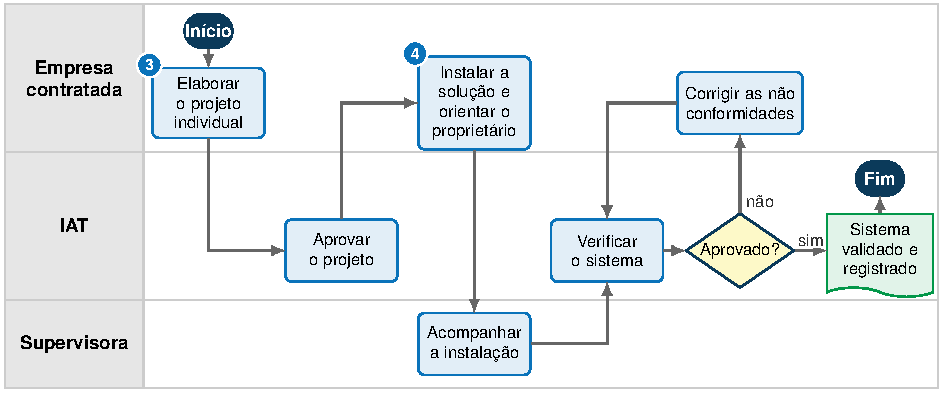
\includegraphics[width=15.96cm]{figuras/f-instalacao.pdf}
  \fonteMOP{Fonte: IAT (2026), com base em IAT (2026b).}
  % Texto alternativo: Fluxograma em raias da empresa contratada, do IAT e da supervisora, do projeto individual à validação do sistema, com a decisão técnica e as correções.
\end{figure}

\textbf{Entradas:} projeto aprovado; autorização do proprietário.

\textbf{Responsáveis:} empresa contratada (executa); supervisora (acompanha); IAT (aprova).

\textbf{Produto:} sistema verificado e validado.

\phantomsection
\subsubsection*{4.5 Etapa 5: Orientação do proprietário}

\textbf{Atividades:} orientação do proprietário, durante a instalação, quanto ao funcionamento do sistema, ao uso adequado, à manutenção preventiva, à limpeza periódica e ao registro da manutenção.

\textbf{Entradas:} sistema em instalação; material de orientação aprovado pelo IAT.

\textbf{Responsáveis:} empresa contratada (executa); IAT (aprova o material); proprietário (participa).

\textbf{Produto:} proprietário orientado, com registro de presença.

\phantomsection
\subsubsection*{4.6 Etapa 6: Medição, comprovação e pagamento}

\textbf{Atividades:} como as soluções são implantadas domicílio a domicílio, o pagamento depende de cadeia de comprovação (Figura~\ref{medicao}). A empresa registra as intervenções em relatórios de medição e reúne as evidências; o proprietário assina o registro de confirmação da execução; o IAT realiza a auditoria documental e as verificações \textit{in loco}; a empresa consolida o relatório de medição final; e o IAT avalia, por amostragem, a qualidade das unidades antes da ordenação da despesa e do pagamento.

\begin{figure}[H]
  \centering
  \caption{Medição, comprovação, verificação e pagamento, por responsável}\label{medicao}
  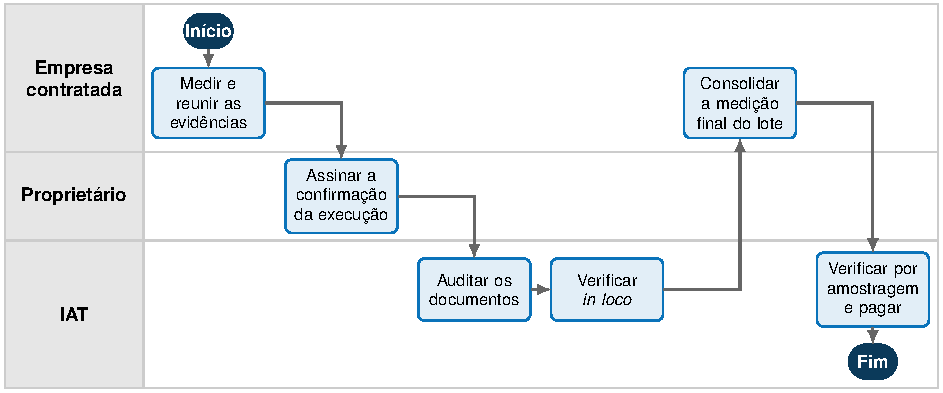
\includegraphics[width=15.96cm]{figuras/f-medicao.pdf}
  \fonteMOP{Fonte: IAT (2026), com base em IAT (2026b).}
  % Texto alternativo: Fluxograma em raias da empresa contratada, do proprietário e do IAT, da medição à amostragem e ao pagamento do lote.
\end{figure}

\textbf{Entradas:} sistemas validados; assinaturas dos proprietários.

\textbf{Responsáveis:} empresa contratada (executa); proprietário (confirma); IAT (verifica, aprova e efetua o pagamento).

\textbf{Produto:} relatório técnico aprovado e comprovante de pagamento, por lote.

\pendencia{Definir o tamanho da amostra da verificação \textit{in loco} e o responsável por cada verificação.}

\phantomsection
\subsubsection*{4.7 Etapa 7: Encerramento}

\textbf{Atividades:} encerramento formal de cada lote e do contrato; consolidação dos resultados para o indicador do componente.

\textbf{Entradas:} relatórios aprovados e pagamentos realizados.

\textbf{Responsáveis:} IAT (executa); UGP (valida).

\textbf{Produto:} lote encerrado.

\phantomsection
\subsubsection*{4.8 Modalidade de execução}

O item de custo é o sistema individual de tratamento de efluentes: 4.067 domicílios a R\$~8.000,00, no total de R\$~32,54 milhões, com recursos do empréstimo do BIRD. A execução ocorre mediante licitação de obras, com o projeto e a instalação no mesmo contrato, conforme o Caderno AQ.

\pendencia{A nota técnica prevê a aquisição centralizada dos materiais pelo IAT, com as obras executadas por empresa contratada; o MOP de março atribuía toda a instalação à empresa. Definir o responsável pela aquisição dos materiais.}

\phantomsection
\addcontentsline{toc}{subsection}{5. Matriz de responsabilidades}
\subsection*{5. Matriz de responsabilidades}

O Quadro~\ref{raci-3225} apresenta o papel de cada parte em cada etapa.

\begin{quadro}[H]
  \caption{Matriz de responsabilidades do esgotamento sanitário nas comunidades}\label{raci-3225}
  \footnotesize\renewcommand{\arraystretch}{1.25}\setlength{\tabcolsep}{3pt}
  \begin{tabular}{>{\raggedright\arraybackslash}p{\dimexpr 0.2536\linewidth-2\tabcolsep\relax}>{\centering\arraybackslash}p{\dimexpr 0.0882\linewidth-2\tabcolsep\relax}>{\centering\arraybackslash}p{\dimexpr 0.0882\linewidth-2\tabcolsep\relax}>{\centering\arraybackslash}p{\dimexpr 0.0882\linewidth-2\tabcolsep\relax}>{\centering\arraybackslash}p{\dimexpr 0.0882\linewidth-2\tabcolsep\relax}>{\centering\arraybackslash}p{\dimexpr 0.0882\linewidth-2\tabcolsep\relax}>{\centering\arraybackslash}p{\dimexpr 0.0882\linewidth-2\tabcolsep\relax}>{\centering\arraybackslash}p{\dimexpr 0.0882\linewidth-2\tabcolsep\relax}>{\centering\arraybackslash}p{\dimexpr 0.1291\linewidth-2\tabcolsep\relax}}
    \rowcolor{azulEscuro}\textcolor{white}{\textbf{Parte}} & \textcolor{white}{\textbf{E1}} & \textcolor{white}{\textbf{E2}} & \textcolor{white}{\textbf{E3}} & \textcolor{white}{\textbf{E4}} & \textcolor{white}{\textbf{E5}} & \textcolor{white}{\textbf{E6}} & \textcolor{white}{\textbf{E7}} & \textcolor{white}{\textbf{Produto final}} \\
    IAT & \raci{R} \raci{A} & \raci{R} \raci{A} & \raci{A} & \raci{A} & \raci{A} & \raci{A} & \raci{R} & \raci{A} \\ \arrayrulecolor{cinza20}\hline
    \rowcolor{cinza5}Empresa contratada & – & – & \raci{R} & \raci{R} & \raci{R} & \raci{R} & \raci{I} & \raci{R} \\ \arrayrulecolor{cinza20}\hline
    Supervisora & – & – & – & \raci{R} & – & \raci{C} & – & – \\ \arrayrulecolor{cinza20}\hline
    \rowcolor{cinza5}Proprietários & \raci{C} & – & \raci{C} & \raci{I} & \raci{R} & \raci{R} & \raci{I} & \raci{I} \\ \arrayrulecolor{cinza20}\hline
    Prefeituras & \raci{I} & – & – & \raci{I} & – & – & \raci{I} & \raci{I} \\ \arrayrulecolor{cinza20}\hline
    \rowcolor{cinza5}UGP & \raci{I} & \raci{C} & \raci{I} & \raci{I} & \raci{I} & \raci{I} & \raci{A} & \raci{I} \\ \arrayrulecolor{cinza20}\hline
    Banco Mundial & – & \raci{C} & – & – & – & – & – & – \\ \noalign{\global\arrayrulewidth=1pt}\arrayrulecolor{azulEscuro}\hline\noalign{\global\arrayrulewidth=0.4pt}
  \end{tabular}
  \fonteMOP{Fonte: IAT (2026).}
  \notaMOP{Nota: E1 a E7 correspondem às Etapas 1 a 7 do item 4. \raci{R} executa (pode haver mais de um); \raci{A} aprova ou valida o produto (um por etapa); \raci{C} é consultado previamente; \raci{I} é informado posteriormente. Produto final: domicílios com solução individual instalada e aprovada.}
\end{quadro}

\phantomsection
\addcontentsline{toc}{subsection}{6. Metas, indicadores e comprovação}
\subsection*{6. Metas, indicadores e comprovação}

O Quadro~\ref{metas-3225} distribui os 4.067 domicílios ao longo do Programa, de forma compatível com o cronograma de implantação dos sistemas de abastecimento.

\begin{quadro}[H]
  \caption{Metas anuais do esgotamento sanitário nas comunidades}\label{metas-3225}
  \footnotesize\renewcommand{\arraystretch}{1.25}\setlength{\tabcolsep}{3pt}
  \begin{tabular}{>{\raggedright\arraybackslash}p{\dimexpr 0.2095\linewidth-2\tabcolsep\relax}>{\raggedright\arraybackslash}p{\dimexpr 0.1268\linewidth-2\tabcolsep\relax}>{\raggedleft\arraybackslash}p{\dimexpr 0.0794\linewidth-2\tabcolsep\relax}>{\raggedleft\arraybackslash}p{\dimexpr 0.0794\linewidth-2\tabcolsep\relax}>{\raggedleft\arraybackslash}p{\dimexpr 0.0794\linewidth-2\tabcolsep\relax}>{\raggedleft\arraybackslash}p{\dimexpr 0.0794\linewidth-2\tabcolsep\relax}>{\raggedleft\arraybackslash}p{\dimexpr 0.0794\linewidth-2\tabcolsep\relax}>{\raggedleft\arraybackslash}p{\dimexpr 0.0794\linewidth-2\tabcolsep\relax}>{\raggedleft\arraybackslash}p{\dimexpr 0.0794\linewidth-2\tabcolsep\relax}>{\raggedleft\arraybackslash}p{\dimexpr 0.1081\linewidth-2\tabcolsep\relax}}
    \rowcolor{azulEscuro}\textcolor{white}{\textbf{Produto}} & \textcolor{white}{\textbf{Unidade}} & \centering\arraybackslash \textcolor{white}{\textbf{Ano 1}} & \centering\arraybackslash \textcolor{white}{\textbf{Ano 2}} & \centering\arraybackslash \textcolor{white}{\textbf{Ano 3}} & \centering\arraybackslash \textcolor{white}{\textbf{Ano 4}} & \centering\arraybackslash \textcolor{white}{\textbf{Ano 5}} & \centering\arraybackslash \textcolor{white}{\textbf{Ano 6}} & \centering\arraybackslash \textcolor{white}{\textbf{Ano 7}} & \centering\arraybackslash \textcolor{white}{\textbf{Total}} \\
    Sistema individual de tratamento de efluentes & domicílios & – & 245 & 477 & 856 & 956 & 956 & 577 & 4.067 \\ \noalign{\global\arrayrulewidth=1pt}\arrayrulecolor{azulEscuro}\hline\noalign{\global\arrayrulewidth=0.4pt}
  \end{tabular}
  \fonteMOP{Fonte: Planilha PSH\_CUSTO\_Consolidada, versão v2408 (PARANÁ, 2026).}
  \notaMOP{Nota: Ano 1 = 2027 e Ano 7 = 2033.}
\end{quadro}

Os indicadores constam do Quadro~\ref{ind-3225}. O indicador do componente corresponde ao número acumulado de domicílios com solução instalada e aprovada multiplicado por 2,8, com desagregação por sexo e para jovens de 15 a 24 anos.

\begin{quadro}[H]
  \caption{Indicadores do esgotamento sanitário nas comunidades}\label{ind-3225}
  \footnotesize\renewcommand{\arraystretch}{1.25}\setlength{\tabcolsep}{3pt}
  \begin{tabular}{>{\raggedright\arraybackslash}p{\dimexpr 0.3165\linewidth-2\tabcolsep\relax}>{\raggedright\arraybackslash}p{\dimexpr 0.1378\linewidth-2\tabcolsep\relax}>{\raggedleft\arraybackslash}p{\dimexpr 0.1102\linewidth-2\tabcolsep\relax}>{\raggedleft\arraybackslash}p{\dimexpr 0.1599\linewidth-2\tabcolsep\relax}>{\raggedright\arraybackslash}p{\dimexpr 0.2756\linewidth-2\tabcolsep\relax}}
    \rowcolor{azulEscuro}\textcolor{white}{\textbf{Indicador}} & \textcolor{white}{\textbf{Unidade}} & \centering\arraybackslash \textcolor{white}{\textbf{Linha de base (2025)}} & \centering\arraybackslash \textcolor{white}{\textbf{Meta}} & \textcolor{white}{\textbf{Frequência e fonte dos dados}} \\
    Domicílios com solução individual instalada e aprovada & domicílios & 0 & 4.067 & Por lote; IAT \\ \arrayrulecolor{cinza20}\hline
    \rowcolor{cinza5}Pessoas atendidas com, pelo menos, esgotamento sanitário (parcela do indicador do componente) & pessoas & 0 & 11.388 & Anual; IAT, com desagregação por sexo e jovens \\ \arrayrulecolor{cinza20}\hline
    Unidades aprovadas na amostragem \textit{in loco} & \% da amostra & – & 100 & Por lote; relatório de amostragem \\ \noalign{\global\arrayrulewidth=1pt}\arrayrulecolor{azulEscuro}\hline\noalign{\global\arrayrulewidth=0.4pt}
  \end{tabular}
  \fonteMOP{Fonte: IAT (2026).}
\end{quadro}

Os critérios de aceite constam do Quadro~\ref{aceite-3225}. A evidência de conclusão de cada lote é o relatório técnico aprovado, acompanhado do comprovante de pagamento.

\begin{quadro}[H]
  \caption{Critérios de aceite e evidências do esgotamento sanitário nas comunidades}\label{aceite-3225}
  \footnotesize\renewcommand{\arraystretch}{1.25}\setlength{\tabcolsep}{5pt}
  \begin{tabular}{>{\raggedright\arraybackslash}p{\dimexpr 0.2150\linewidth-2\tabcolsep\relax}>{\raggedright\arraybackslash}p{\dimexpr 0.3386\linewidth-2\tabcolsep\relax}>{\raggedright\arraybackslash}p{\dimexpr 0.2921\linewidth-2\tabcolsep\relax}>{\raggedright\arraybackslash}p{\dimexpr 0.1543\linewidth-2\tabcolsep\relax}}
    \rowcolor{azulEscuro}\textcolor{white}{\textbf{Produto}} & \textcolor{white}{\textbf{Critério de aceite}} & \textcolor{white}{\textbf{Evidência de comprovação}} & \textcolor{white}{\textbf{Responsável pela validação}} \\
    Projeto individual & Solução adequada ao terreno e ao número de moradores, conforme a ABNT NBR 17076:2024 & Projeto aprovado & IAT \\ \arrayrulecolor{cinza20}\hline
    \rowcolor{cinza5}Sistema instalado & Execução conforme o projeto; teste de estanqueidade aprovado & Relatório de medição; laudo de verificação; registro fotográfico & IAT \\ \arrayrulecolor{cinza20}\hline
    Proprietário orientado & Orientação sobre uso, manutenção e manejo do lodo realizada & Registro de presença & IAT \\ \arrayrulecolor{cinza20}\hline
    \rowcolor{cinza5}Execução confirmada & Execução confirmada pelo proprietário & Assinatura do proprietário & IAT \\ \arrayrulecolor{cinza20}\hline
    Lote aprovado & Auditoria documental, verificação \textit{in loco} e amostragem aprovadas & Relatório técnico aprovado; comprovante de pagamento & IAT \\ \noalign{\global\arrayrulewidth=1pt}\arrayrulecolor{azulEscuro}\hline\noalign{\global\arrayrulewidth=0.4pt}
  \end{tabular}
  \fonteMOP{Fonte: IAT (2026).}
\end{quadro}

\phantomsection
\addcontentsline{toc}{subsection}{7. Gestão de riscos e impactos ambientais e sociais}
\subsection*{7. Gestão de riscos e impactos ambientais e sociais}

Os riscos referem-se à contaminação do solo por instalação inadequada, ao manejo inadequado do lodo, a acidentes durante as obras, à segurança das famílias em razão de valas abertas e à comunicação com os proprietários. As obras ocorrem no interior dos lotes, com autorização do proprietário, sem aquisição de terras (Quadro~\ref{nas-3225}).

\begin{quadro}[H]
  \caption{Aplicação das Normas Ambientais e Sociais ao esgotamento sanitário nas comunidades}\label{nas-3225}
  \footnotesize\renewcommand{\arraystretch}{1.25}\setlength{\tabcolsep}{5pt}
  \begin{tabular}{>{\raggedright\arraybackslash}p{\dimexpr 0.1874\linewidth-2\tabcolsep\relax}>{\raggedright\arraybackslash}p{\dimexpr 0.3716\linewidth-2\tabcolsep\relax}>{\raggedright\arraybackslash}p{\dimexpr 0.4410\linewidth-2\tabcolsep\relax}}
    \rowcolor{azulEscuro}\textcolor{white}{\textbf{NAS}} & \textcolor{white}{\textbf{Aplicação à ação}} & \textcolor{white}{\textbf{Medidas e instrumentos}} \\
    NAS 1 – Avaliação e gestão de riscos & Instalação em cada domicílio & Dimensionamento técnico conforme a ABNT NBR 17076:2024; verificação técnica obrigatória (MGAS) \\ \arrayrulecolor{cinza20}\hline
    \rowcolor{cinza5}NAS 2 – Condições de trabalho & Trabalhadores das empresas contratadas & Uso de EPI; treinamento de segurança; Procedimentos de Gestão de Mão de Obra \\ \arrayrulecolor{cinza20}\hline
    NAS 3 – Eficiência de recursos e prevenção da poluição & Contaminação do solo e da água; lodo e resíduos de obra & Testes de estanqueidade; orientação sobre a limpeza e a destinação do lodo; Plano de Gerenciamento de Resíduos Sólidos \\ \arrayrulecolor{cinza20}\hline
    \rowcolor{cinza5}NAS 4 – Saúde e segurança da comunidade & Valas abertas nos lotes, com circulação de crianças e animais & Sinalização, isolamento e proteção das valas; execução em prazo reduzido em cada domicílio \\ \arrayrulecolor{cinza20}\hline
    NAS 10 – Engajamento das partes interessadas & Proprietários e moradores & Autorização prévia; reuniões com linguagem acessível; Mecanismo de Queixas e Reclamações (PEPI e MQR) \\ \noalign{\global\arrayrulewidth=1pt}\arrayrulecolor{azulEscuro}\hline\noalign{\global\arrayrulewidth=0.4pt}
  \end{tabular}
  \fonteMOP{Fonte: IAT (2026), com base nos instrumentos do Caderno AS.}
  \notaMOP{Nota: a NAS 5 não se aplica, por não haver aquisição de terras; as NAS 6, 7 e 8 são verificadas na triagem das comunidades.}
\end{quadro}

\phantomsection
\addcontentsline{toc}{subsection}{8. Cronograma}
\subsection*{8. Cronograma}

A contratação ocorre em 2028, e os projetos, as instalações, a orientação e as medições, de 2028 a 2033, conforme a planilha de custos: 245 domicílios em 2028, 477 em 2029, 856 em 2030, 956 em 2031 e em 2032 e 577 em 2033 (Figura~\ref{crono-3225}).

\begin{figure}[H]
  \centering
  \caption{Cronograma das etapas e das entregas do esgotamento sanitário nas comunidades}\label{crono-3225}
  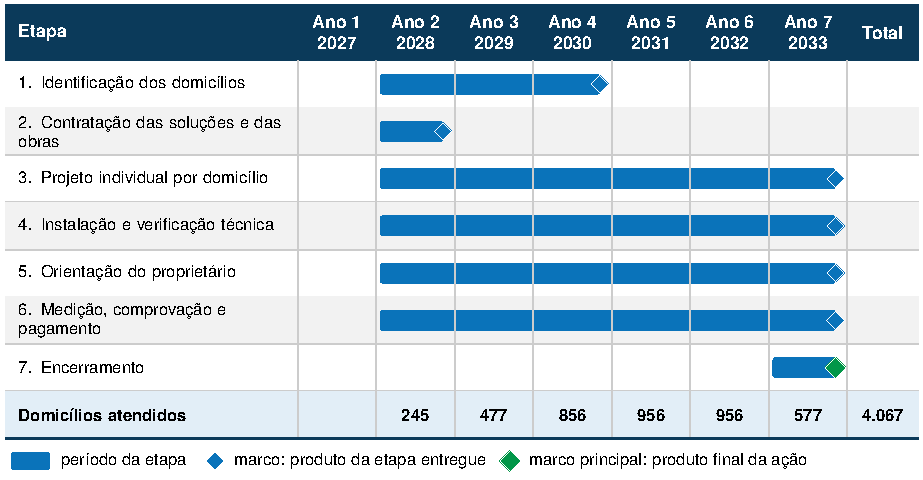
\includegraphics[width=15.64cm]{figuras/g-crono-3225.pdf}
  \fonteMOP{Fonte: IAT (2026), com quantidades da planilha PSH\_CUSTO\_Consolidada (PARANÁ, 2026).}
  % Texto alternativo: Cronograma anual de 2027 a 2033 com as etapas e as quantidades a entregar do esgotamento sanitário nas comunidades.
\end{figure}

\phantomsection
\addcontentsline{toc}{subsection}{9. Interfaces e dependências}
\subsection*{9. Interfaces e dependências}

A ação recebe do trabalho técnico-social o diagnóstico domiciliar e os termos de adesão; da implantação dos sistemas de abastecimento, as comunidades atendidas e o cronograma das obras; e da supervisão das obras, o acompanhamento das instalações. Fornece o número de pessoas atendidas para o indicador do componente e reduz a carga de esgoto lançada no solo e nos corpos hídricos (Figura~\ref{interf-3225}).

\begin{figure}[H]
  \centering
  \caption{Interfaces e dependências do esgotamento sanitário nas comunidades}\label{interf-3225}
  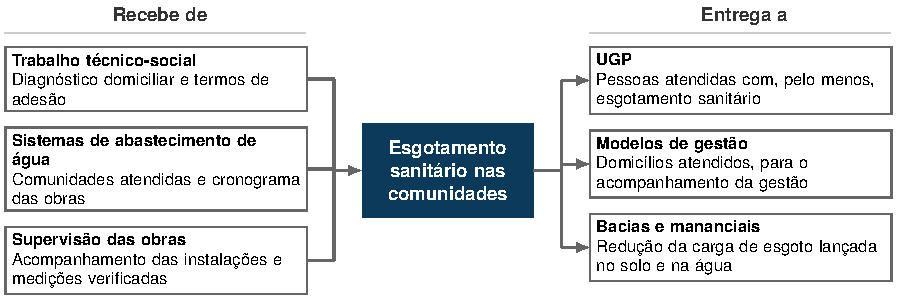
\includegraphics[width=15.30cm]{figuras/g-interf-3225.pdf}
  \fonteMOP{Fonte: IAT (2026).}
  % Texto alternativo: Diagrama das interfaces do esgotamento sanitário nas comunidades: insumos recebidos de outras partes do Programa e produtos entregues a elas.
\end{figure}

\phantomsection
\addcontentsline{toc}{subsection}{10. Documentos complementares}
\subsection*{10. Documentos complementares}

\begin{itemize}
  \item ABNT NBR 17076:2024 (ABNT, 2024);
  \item Termo de Referência e edital das soluções descentralizadas e das obras civis (a elaborar);
  \item Modelo de autorização e de confirmação da execução pelo proprietário (a elaborar);
  \item Material de orientação do proprietário sobre uso, manutenção e manejo do lodo (a elaborar);
  \item Tonetti et al. (2018), referência para a seleção das soluções;
  \item Caderno AQ e Caderno AS.
\end{itemize}

\acao{Ação 3.2.2.6 – Esgotamento sanitário em propriedades de mananciais (área da SEAB)}

\pendencia{Ajuste do nome da ação (Orientações para elaboração dos cadernos, seção 6): “área do IDR-Paraná” passa a “área da SEAB”. A mesma alteração está registrada, em controle de alterações, no quadro de atividades e ações do Subcomponente 3.2. Informar à UGP.}

\phantomsection
\addcontentsline{toc}{subsection}{1. Contextualização}
\subsection*{1. Contextualização}

A ação implanta soluções individuais de esgotamento sanitário em 2.300 domicílios rurais situados em mananciais de abastecimento público da área prioritária do PSH-PR, em propriedades atendidas pela SEAB, entre 2029 e 2033. Além do atendimento a domicílios sem solução, a ação substitui sistemas inadequados de disposição do esgoto (IAT, 2026a).

O esgoto lançado sem tratamento no solo e nos cursos d'água de um manancial compromete a qualidade da água bruta destinada ao abastecimento público, com aporte de matéria orgânica, nutrientes e microrganismos patogênicos. Nos nove mananciais selecionados, 2.236 domicílios particulares permanentes ocupados apresentam destinação inadequada do esgoto, segundo os dados do Censo 2022 e do CNEFE (IAT, 2026a).

A ação reduz a carga poluidora nos mananciais e complementa a gestão de riscos nas bacias de abastecimento público, no próprio componente, e as práticas agropecuárias implantadas nas mesmas propriedades no Componente 2. Contribui também para o indicador de pessoas atendidas com, pelo menos, esgotamento sanitário, com cerca de 6,4 mil pessoas.

\textbf{Inclui:} a indicação dos domicílios pela SEAB; a contratação das soluções e das obras; o projeto sanitário de cada propriedade; a instalação conforme a ABNT NBR 17076:2024; a verificação técnica; a orientação do proprietário; e a medição, a comprovação e o pagamento, com validação técnica do IAT e da SEAB.

\textbf{Não inclui:} a elaboração dos Planos Integrados de Propriedade (PIP), realizada no Componente 2, nem redes coletoras ou intervenções no interior das moradias.

\textbf{Valor previsto:} R\$~18,40 milhões (empréstimo BIRD: R\$~18,40 milhões; contrapartida: R\$~0,00 milhões), conforme a planilha PSH\_CUSTO\_Consolidada.

\phantomsection
\addcontentsline{toc}{subsection}{2. Área de atuação}
\subsection*{2. Área de atuação}

A área de atuação resulta da aplicação sucessiva de critérios (Figura~\ref{selecao-mananciais}): microbacias prioritárias do PSH-PR; mananciais de abastecimento público selecionados por critérios de qualidade e de quantidade da água; domicílios rurais permanentes ocupados; ausência de destinação adequada do esgoto, segundo o Censo 2022; e existência de diagnóstico da microbacia e de adesão da propriedade ao PSH-PR e às ações da SEAB (IAT, 2026a).

\begin{figure}[H]
  \centering
  \caption{Critérios de seleção dos domicílios em mananciais}\label{selecao-mananciais}
  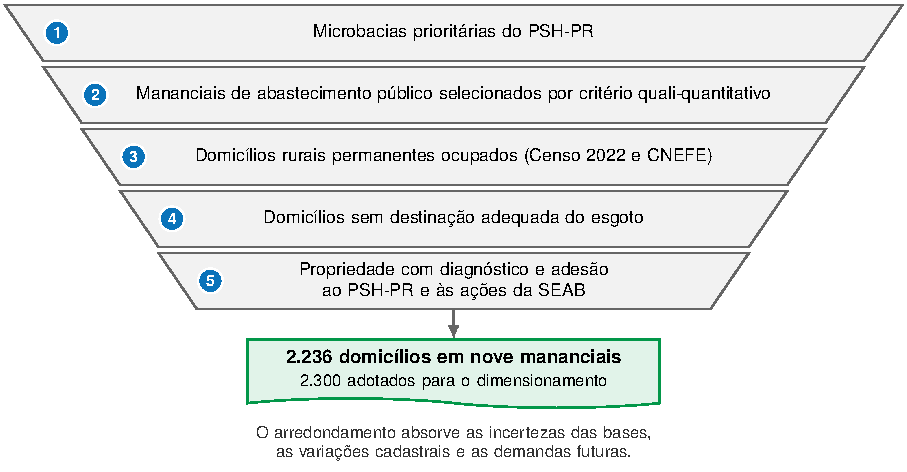
\includegraphics[width=15.37cm]{figuras/f-selecao-mananciais.pdf}
  \fonteMOP{Fonte: IAT (2026), com base em IAT (2026a).}
  % Texto alternativo: Funil com os cinco critérios de seleção dos domicílios em mananciais, que resulta em 2.236 domicílios e na meta de 2.300.
\end{figure}

A aplicação dos critérios resultou em 2.236 domicílios com esgotamento inadequado em nove mananciais, dos quais 1.925 no manancial do Rio Pirapó (Tabela~\ref{mananciais}). Para o dimensionamento da ação, o número foi arredondado para 2.300 domicílios, margem que absorve as incertezas das bases de dados, as variações cadastrais e as demandas futuras.

\begin{table}[H]
  \caption{Domicílios com esgotamento inadequado nos mananciais selecionados}\label{mananciais}
  \footnotesize\renewcommand{\arraystretch}{1.25}\setlength{\tabcolsep}{5pt}
  \begin{tabular}{>{\raggedright\arraybackslash}p{\dimexpr 0.3197\linewidth-2\tabcolsep\relax}>{\raggedright\arraybackslash}p{\dimexpr 0.2095\linewidth-2\tabcolsep\relax}>{\raggedleft\arraybackslash}p{\dimexpr 0.1874\linewidth-2\tabcolsep\relax}>{\raggedleft\arraybackslash}p{\dimexpr 0.1874\linewidth-2\tabcolsep\relax}>{\raggedleft\arraybackslash}p{\dimexpr 0.0960\linewidth-2\tabcolsep\relax}}
    \rowcolor{azulEscuro}\textcolor{white}{\textbf{Manancial}} & \textcolor{white}{\textbf{Critério}} & \centering\arraybackslash \textcolor{white}{\textbf{Domicílios permanentes}} & \centering\arraybackslash \textcolor{white}{\textbf{Esgotamento inadequado}} & \centering\arraybackslash \textcolor{white}{\textbf{\%}} \\
    Rio Marumbi & Qualitativo & 128 & 120 & 94 \\ \arrayrulecolor{cinza20}\hline
    \rowcolor{cinza5}Rio Pirapó & Qualitativo & 2.750 & 1.925 & 70 \\ \arrayrulecolor{cinza20}\hline
    Ribeirão Floresta & Qualitativo & 17 & 17 & 100 \\ \arrayrulecolor{cinza20}\hline
    \rowcolor{cinza5}Rio Palmital & Qualitativo & 20 & 16 & 80 \\ \arrayrulecolor{cinza20}\hline
    Ribeirão Paracatu & Qualitativo & 17 & 17 & 100 \\ \arrayrulecolor{cinza20}\hline
    \rowcolor{cinza5}Ribeirão Guarazinho & Qualitativo & 22 & 22 & 100 \\ \arrayrulecolor{cinza20}\hline
    Rio Água Grande & Qualitativo & 91 & 53 & 58 \\ \arrayrulecolor{cinza20}\hline
    \rowcolor{cinza5}Ribeirão Água na Campina & Qualitativo & 37 & 37 & 100 \\ \arrayrulecolor{cinza20}\hline
    Ribeirão do Noitimbo & Quali-quantitativo & 29 & 29 & 100 \\ \arrayrulecolor{cinza20}\hline
    \rowcolor{petroleo12}\textbf{Total} &  & \textbf{3.111} & \textbf{2.236} & \textbf{72} \\ \noalign{\global\arrayrulewidth=1pt}\arrayrulecolor{azulEscuro}\hline\noalign{\global\arrayrulewidth=0.4pt}
  \end{tabular}
  \fonteMOP{Fonte: Adaptado de IAT (2026a), com dados do Censo Demográfico 2022 agregados por setor censitário e do CNEFE (IBGE, 2024).}
  \notaMOP{Nota: domicílios particulares permanentes ocupados. Para o dimensionamento, adotaram-se 2.300 domicílios.}
\end{table}

\pendencia{Na tabela da nota técnica, o Rio Marumbi consta com 90\%, mas 120 de 128 domicílios correspondem a 94\%. Conferir.}

\pendencia{O Acordo de Empréstimo, item (j)(vii) das definições, exige a identificação das áreas rurais da Parte 3.2. Incluir o mapa dos nove mananciais, com as microbacias e os municípios.}

\phantomsection
\addcontentsline{toc}{subsection}{3. Arranjo institucional e partes interessadas}
\subsection*{3. Arranjo institucional e partes interessadas}

O IAT, por meio da DISAR, contrata a empresa, fiscaliza a instalação e efetua o pagamento, com apoio da supervisora das obras. A SEAB indica os domicílios a partir dos PIP, apoia a mobilização dos proprietários e participa da validação técnica dos resultados. A empresa contratada elabora o projeto de cada propriedade e executa a instalação, e o proprietário autoriza, acompanha e confirma a execução.

\begin{itemize}
  \item \textbf{Coexecutora:} SEAB, na indicação dos domicílios, na mobilização e na validação técnica;
  \item \textbf{Intervenientes:} empresa contratada; empresa supervisora das obras; UGP, que acompanha a execução;
  \item \textbf{Público envolvido:} proprietários e moradores das propriedades rurais dos mananciais.
\end{itemize}

Os beneficiários diretos são os moradores dos 2.300 domicílios, cerca de 6,4 mil pessoas. Os beneficiários indiretos são as populações abastecidas pelos mananciais, com a melhoria da qualidade da água bruta.

\phantomsection
\addcontentsline{toc}{subsection}{4. Processo de execução operacional}
\subsection*{4. Processo de execução operacional}

A ação adota o mesmo procedimento de instalação, verificação, medição e pagamento do esgotamento sanitário nas comunidades (Figura~\ref{instalacao} e Figura~\ref{medicao}), com as etapas por responsável apresentadas na Figura~\ref{raias-3226}. As diferenças referem-se à origem da demanda, ao território e à validação (Quadro~\ref{diferencas}): os domicílios são indicados pela SEAB a partir dos PIP, e não pelo trabalho técnico-social; o território corresponde aos mananciais de abastecimento público; e a validação técnica de cada lote conta com a participação da SEAB.

\begin{quadro}[H]
  \caption{Diferenças entre as ações de esgotamento sanitário}\label{diferencas}
  \footnotesize\renewcommand{\arraystretch}{1.25}\setlength{\tabcolsep}{5pt}
  \begin{tabular}{>{\raggedright\arraybackslash}p{\dimexpr 0.2425\linewidth-2\tabcolsep\relax}>{\raggedright\arraybackslash}p{\dimexpr 0.3787\linewidth-2\tabcolsep\relax}>{\raggedright\arraybackslash}p{\dimexpr 0.3788\linewidth-2\tabcolsep\relax}}
    \rowcolor{azulEscuro}\textcolor{white}{\textbf{Aspecto}} & \textcolor{white}{\textbf{Esgotamento sanitário nas comunidades}} & \textcolor{white}{\textbf{Esgotamento sanitário em mananciais}} \\
    Origem da demanda & Diagnóstico do trabalho técnico-social & PIP, com indicação dos domicílios pela SEAB \\ \arrayrulecolor{cinza20}\hline
    \rowcolor{cinza5}Território & Comunidades atendidas pelos sistemas de abastecimento de água & Nove mananciais da área prioritária do PSH-PR \\ \arrayrulecolor{cinza20}\hline
    Base do levantamento & Censo 2022 e CNEFE: 70\% dos 5.810 domicílios sem esgotamento adequado & Censo 2022 e CNEFE: 2.236 domicílios, arredondados para 2.300 \\ \arrayrulecolor{cinza20}\hline
    \rowcolor{cinza5}Meta & 4.067 domicílios & 2.300 domicílios \\ \arrayrulecolor{cinza20}\hline
    Prazo & 2028 a 2033 & 2029 a 2033 \\ \arrayrulecolor{cinza20}\hline
    \rowcolor{cinza5}Validação & IAT & IAT, com a SEAB \\ \noalign{\global\arrayrulewidth=1pt}\arrayrulecolor{azulEscuro}\hline\noalign{\global\arrayrulewidth=0.4pt}
  \end{tabular}
  \fonteMOP{Fonte: IAT (2026), com base em IAT (2026a) e PARANÁ (2026).}
\end{quadro}

\begin{figure}[H]
  \centering
  \caption{Fluxograma do esgotamento sanitário em mananciais: entradas, etapas por responsável e saídas}\label{raias-3226}
  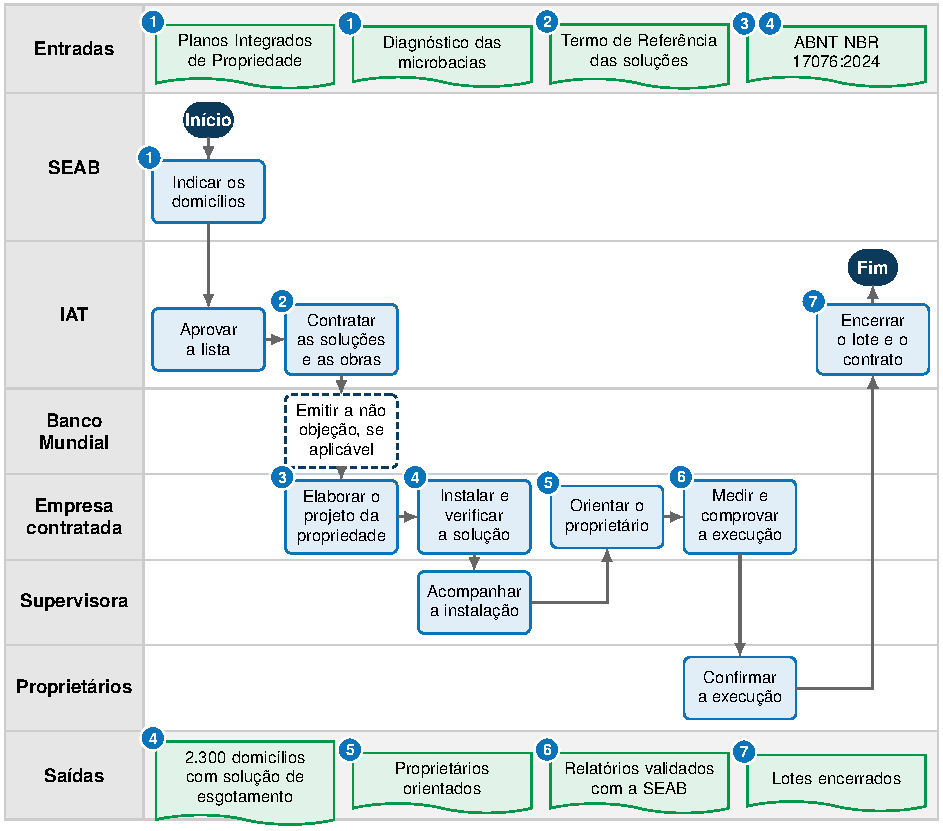
\includegraphics[width=15.96cm]{figuras/g-raias-3226.pdf}
  \fonteMOP{Fonte: IAT (2026).}
  % Texto alternativo: Fluxograma em raias do esgotamento sanitário em mananciais, com uma raia por instituição, as etapas numeradas na raia do executor, as entradas no topo e as saídas na base.
\end{figure}

\phantomsection
\subsubsection*{4.1 Etapa 1: Indicação dos domicílios pela SEAB}

\textbf{Atividades:} indicação pela SEAB, a partir dos PIP e do diagnóstico das microbacias, dos domicílios sem destinação adequada do esgoto; confirmação da adesão e autorização da intervenção pelo proprietário.

\textbf{Entradas:} PIP; diagnóstico das microbacias; critérios do item 2.

\textbf{Responsáveis:} SEAB (executa); IAT (aprova a lista); proprietários (consultados).

\textbf{Produto:} lista de domicílios por manancial.

\pendencia{Confirmar o cronograma dos PIP no Componente 2, que condiciona o início das instalações em 2029.}

\phantomsection
\subsubsection*{4.2 Etapa 2: Contratação das soluções e das obras}

\textbf{Atividades:} elaboração do Termo de Referência das soluções descentralizadas e das obras civis; publicação do edital; licitação; contratação. A contratação pode integrar o processo do esgotamento sanitário nas comunidades, em lotes próprios.

\textbf{Entradas:} lista de domicílios; especificações conforme a ABNT NBR 17076:2024.

\textbf{Responsáveis:} IAT (executa e aprova); SEAB (consultada); UGP e Banco Mundial (consultados, quando houver revisão prévia).

\textbf{Produto:} contrato assinado.

\phantomsection
\subsubsection*{4.3 Etapa 3: Projeto sanitário da propriedade}

\textbf{Atividades:} elaboração, pela empresa contratada, do projeto de cada propriedade, considerada a topografia do terreno, o número de moradores, a capacidade de infiltração do solo e a solução de tratamento adequada, inclusive o manejo do lodo.

\textbf{Entradas:} contrato; dados do PIP.

\textbf{Responsáveis:} empresa contratada (executa); IAT (aprova); SEAB e proprietário (consultados).

\textbf{Produto:} projeto aprovado.

\phantomsection
\subsubsection*{4.4 Etapa 4: Instalação e verificação técnica}

\textbf{Atividades:} execução das obras civis e instalação dos dispositivos; verificação do funcionamento, da estanqueidade e da garantia; correções, quando necessárias, conforme a Figura~\ref{instalacao}.

\textbf{Entradas:} projeto aprovado; autorização do proprietário.

\textbf{Responsáveis:} empresa contratada (executa); supervisora (acompanha); IAT (aprova).

\textbf{Produto:} sistema verificado e validado.

\phantomsection
\subsubsection*{4.5 Etapa 5: Orientação do proprietário}

\textbf{Atividades:} orientação quanto ao funcionamento, ao uso adequado, à manutenção preventiva e à limpeza periódica, durante a instalação, com apoio da equipe técnica da SEAB que atende a propriedade.

\textbf{Entradas:} sistema em instalação; material de orientação.

\textbf{Responsáveis:} empresa contratada (executa); SEAB (consultada); IAT (aprova o material).

\textbf{Produto:} proprietário orientado.

\phantomsection
\subsubsection*{4.6 Etapa 6: Medição, comprovação e pagamento}

\textbf{Atividades:} relatórios de medição e evidências; assinatura do proprietário; auditoria documental e verificação \textit{in loco}; relatório de medição final; amostragem \textit{in loco}; ordenação da despesa e pagamento, conforme a Figura~\ref{medicao}. O IAT aprova cada lote após a validação técnica realizada com a SEAB.

\textbf{Entradas:} sistemas validados; assinaturas dos proprietários.

\textbf{Responsáveis:} empresa contratada (executa); SEAB (consultada na validação); IAT (aprova e efetua o pagamento).

\textbf{Produto:} relatório técnico aprovado pelo IAT, com a validação da SEAB, e comprovante de pagamento, por lote.

\pendencia{A nota técnica prevê validação conjunta. Na matriz, a SEAB figura como C (consultada antes da aprovação), porque o Guia de Identidade Visual admite um único A por etapa. Confirmar o papel com a SEAB e registrá-lo no protocolo de validação.}

\phantomsection
\subsubsection*{4.7 Etapa 7: Encerramento}

\textbf{Atividades:} encerramento de cada lote e do contrato; registro das propriedades atendidas, para a assistência técnica prestada pela SEAB.

\textbf{Entradas:} relatórios aprovados e pagamentos realizados.

\textbf{Responsáveis:} IAT (executa); UGP (valida).

\textbf{Produto:} lote encerrado.

\phantomsection
\subsubsection*{4.8 Modalidade de execução}

O item de custo é o sistema individual de tratamento de efluentes: 2.300 domicílios a R\$~8.000,00, no total de R\$~18,40 milhões, com recursos do empréstimo do BIRD. A execução ocorre mediante licitação de obras, com o projeto e a instalação no mesmo contrato, conforme o Caderno AQ. O eventual agrupamento com o esgotamento sanitário nas comunidades em um mesmo processo, em lotes distintos, é definido no Plano de Aquisições.

\phantomsection
\addcontentsline{toc}{subsection}{5. Matriz de responsabilidades}
\subsection*{5. Matriz de responsabilidades}

O Quadro~\ref{raci-3226} apresenta o papel de cada parte em cada etapa.

\begin{quadro}[H]
  \caption{Matriz de responsabilidades do esgotamento sanitário em mananciais}\label{raci-3226}
  \footnotesize\renewcommand{\arraystretch}{1.25}\setlength{\tabcolsep}{3pt}
  \begin{tabular}{>{\raggedright\arraybackslash}p{\dimexpr 0.2536\linewidth-2\tabcolsep\relax}>{\centering\arraybackslash}p{\dimexpr 0.0882\linewidth-2\tabcolsep\relax}>{\centering\arraybackslash}p{\dimexpr 0.0882\linewidth-2\tabcolsep\relax}>{\centering\arraybackslash}p{\dimexpr 0.0882\linewidth-2\tabcolsep\relax}>{\centering\arraybackslash}p{\dimexpr 0.0882\linewidth-2\tabcolsep\relax}>{\centering\arraybackslash}p{\dimexpr 0.0882\linewidth-2\tabcolsep\relax}>{\centering\arraybackslash}p{\dimexpr 0.0882\linewidth-2\tabcolsep\relax}>{\centering\arraybackslash}p{\dimexpr 0.0882\linewidth-2\tabcolsep\relax}>{\centering\arraybackslash}p{\dimexpr 0.1291\linewidth-2\tabcolsep\relax}}
    \rowcolor{azulEscuro}\textcolor{white}{\textbf{Parte}} & \textcolor{white}{\textbf{E1}} & \textcolor{white}{\textbf{E2}} & \textcolor{white}{\textbf{E3}} & \textcolor{white}{\textbf{E4}} & \textcolor{white}{\textbf{E5}} & \textcolor{white}{\textbf{E6}} & \textcolor{white}{\textbf{E7}} & \textcolor{white}{\textbf{Produto final}} \\
    IAT & \raci{A} & \raci{R} \raci{A} & \raci{A} & \raci{A} & \raci{A} & \raci{A} & \raci{R} & \raci{A} \\ \arrayrulecolor{cinza20}\hline
    \rowcolor{cinza5}SEAB & \raci{R} & \raci{C} & \raci{C} & \raci{I} & \raci{C} & \raci{C} & \raci{I} & \raci{C} \\ \arrayrulecolor{cinza20}\hline
    Empresa contratada & – & – & \raci{R} & \raci{R} & \raci{R} & \raci{R} & \raci{I} & \raci{R} \\ \arrayrulecolor{cinza20}\hline
    \rowcolor{cinza5}Supervisora & – & – & – & \raci{R} & – & \raci{C} & – & – \\ \arrayrulecolor{cinza20}\hline
    Proprietários & \raci{C} & – & \raci{C} & \raci{I} & \raci{R} & \raci{R} & \raci{I} & \raci{I} \\ \arrayrulecolor{cinza20}\hline
    \rowcolor{cinza5}UGP & \raci{I} & \raci{C} & \raci{I} & \raci{I} & \raci{I} & \raci{I} & \raci{A} & \raci{I} \\ \arrayrulecolor{cinza20}\hline
    Banco Mundial & – & \raci{C} & – & – & – & – & – & – \\ \noalign{\global\arrayrulewidth=1pt}\arrayrulecolor{azulEscuro}\hline\noalign{\global\arrayrulewidth=0.4pt}
  \end{tabular}
  \fonteMOP{Fonte: IAT (2026).}
  \notaMOP{Nota: E1 a E7 correspondem às Etapas 1 a 7 do item 4. \raci{R} executa (pode haver mais de um); \raci{A} aprova ou valida o produto (um por etapa); \raci{C} é consultado previamente; \raci{I} é informado posteriormente. Produto final: domicílios dos mananciais com solução individual instalada e aprovada.}
\end{quadro}

\phantomsection
\addcontentsline{toc}{subsection}{6. Metas, indicadores e comprovação}
\subsection*{6. Metas, indicadores e comprovação}

A meta é de 460 domicílios por ano, de 2029 a 2033 (Quadro~\ref{metas-3226}).

\begin{quadro}[H]
  \caption{Metas anuais do esgotamento sanitário em mananciais}\label{metas-3226}
  \footnotesize\renewcommand{\arraystretch}{1.25}\setlength{\tabcolsep}{3pt}
  \begin{tabular}{>{\raggedright\arraybackslash}p{\dimexpr 0.2095\linewidth-2\tabcolsep\relax}>{\raggedright\arraybackslash}p{\dimexpr 0.1268\linewidth-2\tabcolsep\relax}>{\raggedleft\arraybackslash}p{\dimexpr 0.0794\linewidth-2\tabcolsep\relax}>{\raggedleft\arraybackslash}p{\dimexpr 0.0794\linewidth-2\tabcolsep\relax}>{\raggedleft\arraybackslash}p{\dimexpr 0.0794\linewidth-2\tabcolsep\relax}>{\raggedleft\arraybackslash}p{\dimexpr 0.0794\linewidth-2\tabcolsep\relax}>{\raggedleft\arraybackslash}p{\dimexpr 0.0794\linewidth-2\tabcolsep\relax}>{\raggedleft\arraybackslash}p{\dimexpr 0.0794\linewidth-2\tabcolsep\relax}>{\raggedleft\arraybackslash}p{\dimexpr 0.0794\linewidth-2\tabcolsep\relax}>{\raggedleft\arraybackslash}p{\dimexpr 0.1081\linewidth-2\tabcolsep\relax}}
    \rowcolor{azulEscuro}\textcolor{white}{\textbf{Produto}} & \textcolor{white}{\textbf{Unidade}} & \centering\arraybackslash \textcolor{white}{\textbf{Ano 1}} & \centering\arraybackslash \textcolor{white}{\textbf{Ano 2}} & \centering\arraybackslash \textcolor{white}{\textbf{Ano 3}} & \centering\arraybackslash \textcolor{white}{\textbf{Ano 4}} & \centering\arraybackslash \textcolor{white}{\textbf{Ano 5}} & \centering\arraybackslash \textcolor{white}{\textbf{Ano 6}} & \centering\arraybackslash \textcolor{white}{\textbf{Ano 7}} & \centering\arraybackslash \textcolor{white}{\textbf{Total}} \\
    Sistema individual de tratamento de efluentes & domicílios & – & – & 460 & 460 & 460 & 460 & 460 & 2.300 \\ \noalign{\global\arrayrulewidth=1pt}\arrayrulecolor{azulEscuro}\hline\noalign{\global\arrayrulewidth=0.4pt}
  \end{tabular}
  \fonteMOP{Fonte: Planilha PSH\_CUSTO\_Consolidada, versão v2408 (PARANÁ, 2026).}
  \notaMOP{Nota: Ano 1 = 2027 e Ano 7 = 2033.}
\end{quadro}

Os indicadores constam do Quadro~\ref{ind-3226}; o de pessoas atendidas é calculado da mesma forma que no esgotamento sanitário nas comunidades.

\begin{quadro}[H]
  \caption{Indicadores do esgotamento sanitário em mananciais}\label{ind-3226}
  \footnotesize\renewcommand{\arraystretch}{1.25}\setlength{\tabcolsep}{3pt}
  \begin{tabular}{>{\raggedright\arraybackslash}p{\dimexpr 0.3165\linewidth-2\tabcolsep\relax}>{\raggedright\arraybackslash}p{\dimexpr 0.1378\linewidth-2\tabcolsep\relax}>{\raggedleft\arraybackslash}p{\dimexpr 0.1102\linewidth-2\tabcolsep\relax}>{\raggedleft\arraybackslash}p{\dimexpr 0.1599\linewidth-2\tabcolsep\relax}>{\raggedright\arraybackslash}p{\dimexpr 0.2756\linewidth-2\tabcolsep\relax}}
    \rowcolor{azulEscuro}\textcolor{white}{\textbf{Indicador}} & \textcolor{white}{\textbf{Unidade}} & \centering\arraybackslash \textcolor{white}{\textbf{Linha de base (2025)}} & \centering\arraybackslash \textcolor{white}{\textbf{Meta}} & \textcolor{white}{\textbf{Frequência e fonte dos dados}} \\
    Domicílios de mananciais com solução individual instalada e aprovada & domicílios & 0 & 2.300 & Por lote; IAT e SEAB \\ \arrayrulecolor{cinza20}\hline
    \rowcolor{cinza5}Pessoas atendidas com, pelo menos, esgotamento sanitário (parcela do indicador do componente) & pessoas & 0 & 6.440 & Anual; IAT, com desagregação por sexo e jovens \\ \arrayrulecolor{cinza20}\hline
    Mananciais com instalações concluídas & mananciais & 0 & 9 & Anual; IAT \\ \noalign{\global\arrayrulewidth=1pt}\arrayrulecolor{azulEscuro}\hline\noalign{\global\arrayrulewidth=0.4pt}
  \end{tabular}
  \fonteMOP{Fonte: IAT (2026).}
\end{quadro}

Os critérios de aceite são os mesmos do esgotamento sanitário nas comunidades, com validação técnica realizada com a SEAB (Quadro~\ref{aceite-3226}).

\begin{quadro}[H]
  \caption{Critérios de aceite e evidências do esgotamento sanitário em mananciais}\label{aceite-3226}
  \footnotesize\renewcommand{\arraystretch}{1.25}\setlength{\tabcolsep}{5pt}
  \begin{tabular}{>{\raggedright\arraybackslash}p{\dimexpr 0.2150\linewidth-2\tabcolsep\relax}>{\raggedright\arraybackslash}p{\dimexpr 0.3386\linewidth-2\tabcolsep\relax}>{\raggedright\arraybackslash}p{\dimexpr 0.2921\linewidth-2\tabcolsep\relax}>{\raggedright\arraybackslash}p{\dimexpr 0.1543\linewidth-2\tabcolsep\relax}}
    \rowcolor{azulEscuro}\textcolor{white}{\textbf{Produto}} & \textcolor{white}{\textbf{Critério de aceite}} & \textcolor{white}{\textbf{Evidência de comprovação}} & \textcolor{white}{\textbf{Responsável pela validação}} \\
    Lista de domicílios & Domicílios dos mananciais sem destinação adequada, com adesão do proprietário & Lista da SEAB, com os PIP de origem & IAT \\ \arrayrulecolor{cinza20}\hline
    \rowcolor{cinza5}Projeto sanitário & Solução adequada à propriedade, conforme a ABNT NBR 17076:2024 & Projeto aprovado & IAT \\ \arrayrulecolor{cinza20}\hline
    Sistema instalado & Execução conforme o projeto; teste de estanqueidade aprovado & Relatório de medição; laudo de verificação; registro fotográfico & IAT, com a SEAB \\ \arrayrulecolor{cinza20}\hline
    \rowcolor{cinza5}Execução confirmada & Execução confirmada pelo proprietário & Assinatura do proprietário & IAT \\ \arrayrulecolor{cinza20}\hline
    Lote aprovado & Auditoria documental, verificação \textit{in loco} e amostragem aprovadas & Relatório técnico aprovado; comprovante de pagamento & IAT, com a SEAB \\ \noalign{\global\arrayrulewidth=1pt}\arrayrulecolor{azulEscuro}\hline\noalign{\global\arrayrulewidth=0.4pt}
  \end{tabular}
  \fonteMOP{Fonte: IAT (2026).}
\end{quadro}

\phantomsection
\addcontentsline{toc}{subsection}{7. Gestão de riscos e impactos ambientais e sociais}
\subsection*{7. Gestão de riscos e impactos ambientais e sociais}

Os riscos são os mesmos do esgotamento sanitário nas comunidades, com atenção adicional à proteção dos recursos hídricos, por se tratar de instalações em mananciais de abastecimento público (Quadro~\ref{nas-3226}).

\begin{quadro}[H]
  \caption{Aplicação das Normas Ambientais e Sociais ao esgotamento sanitário em mananciais}\label{nas-3226}
  \footnotesize\renewcommand{\arraystretch}{1.25}\setlength{\tabcolsep}{5pt}
  \begin{tabular}{>{\raggedright\arraybackslash}p{\dimexpr 0.1874\linewidth-2\tabcolsep\relax}>{\raggedright\arraybackslash}p{\dimexpr 0.3716\linewidth-2\tabcolsep\relax}>{\raggedright\arraybackslash}p{\dimexpr 0.4410\linewidth-2\tabcolsep\relax}}
    \rowcolor{azulEscuro}\textcolor{white}{\textbf{NAS}} & \textcolor{white}{\textbf{Aplicação à ação}} & \textcolor{white}{\textbf{Medidas e instrumentos}} \\
    NAS 1 – Avaliação e gestão de riscos & Instalação em propriedades de mananciais & Dimensionamento conforme a ABNT NBR 17076:2024; distâncias mínimas de nascentes e cursos d'água; verificação técnica (MGAS) \\ \arrayrulecolor{cinza20}\hline
    \rowcolor{cinza5}NAS 2 – Condições de trabalho & Trabalhadores das empresas contratadas & Uso de EPI; treinamento de segurança; Procedimentos de Gestão de Mão de Obra \\ \arrayrulecolor{cinza20}\hline
    NAS 3 – Eficiência de recursos e prevenção da poluição & Contaminação do solo e da água do manancial; lodo & Testes de estanqueidade; orientação sobre o manejo do lodo; Plano de Gerenciamento de Resíduos Sólidos \\ \arrayrulecolor{cinza20}\hline
    \rowcolor{cinza5}NAS 4 – Saúde e segurança da comunidade & Valas abertas nas propriedades & Sinalização, isolamento e proteção das valas \\ \arrayrulecolor{cinza20}\hline
    NAS 10 – Engajamento das partes interessadas & Proprietários rurais & Autorização prévia; apoio da equipe técnica da SEAB; Mecanismo de Queixas e Reclamações (PEPI e MQR) \\ \noalign{\global\arrayrulewidth=1pt}\arrayrulecolor{azulEscuro}\hline\noalign{\global\arrayrulewidth=0.4pt}
  \end{tabular}
  \fonteMOP{Fonte: IAT (2026), com base nos instrumentos do Caderno AS.}
  \notaMOP{Nota: a NAS 5 não se aplica, por não haver aquisição de terras; a NAS 6 é verificada na triagem das propriedades situadas em áreas de preservação.}
\end{quadro}

\phantomsection
\addcontentsline{toc}{subsection}{8. Cronograma}
\subsection*{8. Cronograma}

A SEAB indica os domicílios a partir de 2028, a contratação ocorre em 2029 e as instalações estendem-se de 2029 a 2033, com 460 domicílios por ano (Figura~\ref{crono-3226}).

\begin{figure}[H]
  \centering
  \caption{Cronograma das etapas e das entregas do esgotamento sanitário em mananciais}\label{crono-3226}
  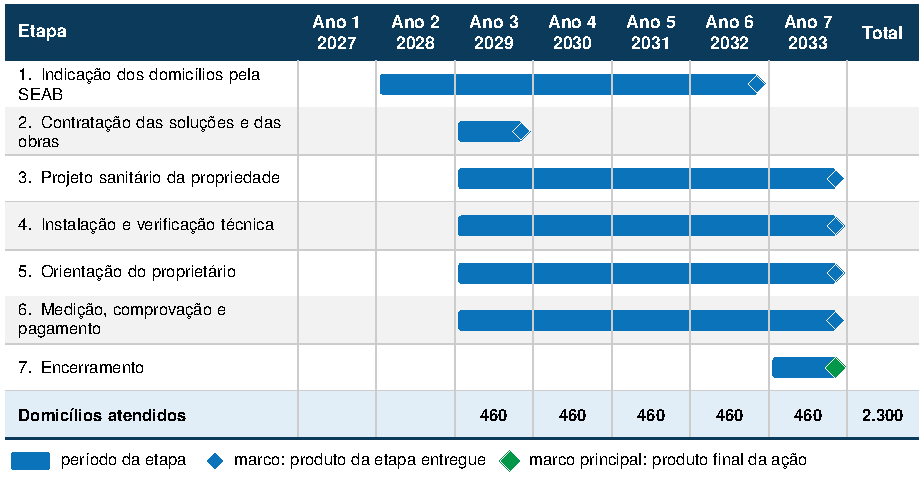
\includegraphics[width=15.64cm]{figuras/g-crono-3226.pdf}
  \fonteMOP{Fonte: IAT (2026), com quantidades da planilha PSH\_CUSTO\_Consolidada (PARANÁ, 2026).}
  % Texto alternativo: Cronograma anual de 2027 a 2033 com as etapas e as quantidades a entregar do esgotamento sanitário em mananciais.
\end{figure}

\phantomsection
\addcontentsline{toc}{subsection}{9. Interfaces e dependências}
\subsection*{9. Interfaces e dependências}

A ação depende dos PIP e do diagnóstico das microbacias, elaborados no Componente 2, e da supervisão das instalações. Fornece à gestão de riscos nas bacias de abastecimento a redução da carga de esgoto nos mananciais, à UGP o número de pessoas atendidas para o indicador do componente e à SEAB o registro das propriedades atendidas (Figura~\ref{interf-3226}).

\begin{figure}[H]
  \centering
  \caption{Interfaces e dependências do esgotamento sanitário em mananciais}\label{interf-3226}
  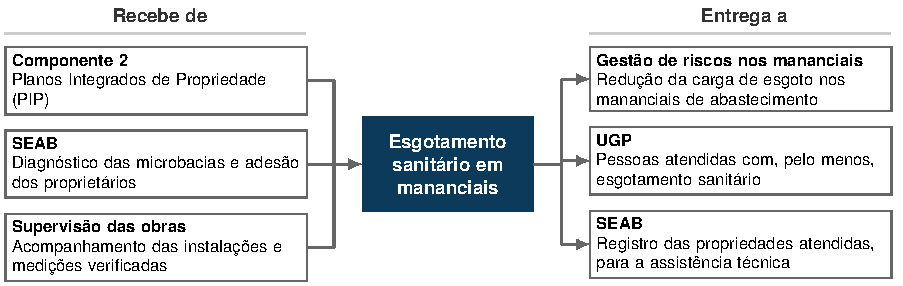
\includegraphics[width=15.30cm]{figuras/g-interf-3226.pdf}
  \fonteMOP{Fonte: IAT (2026).}
  % Texto alternativo: Diagrama das interfaces do esgotamento sanitário em mananciais: insumos recebidos de outras partes do Programa e produtos entregues a elas.
\end{figure}

\phantomsection
\addcontentsline{toc}{subsection}{10. Documentos complementares}
\subsection*{10. Documentos complementares}

\begin{itemize}
  \item ABNT NBR 17076:2024 (ABNT, 2024);
  \item Planos Integrados de Propriedade (Componente 2);
  \item Protocolo de validação técnica IAT–SEAB (a elaborar);
  \item Termo de Referência e edital das soluções e das obras (a elaborar);
  \item Caderno AQ e Caderno AS.
\end{itemize}

\acao{Ação 3.2.2.7 – Supervisão e gerenciamento das obras}

\phantomsection
\addcontentsline{toc}{subsection}{1. Contextualização}
\subsection*{1. Contextualização}

A ação contrata empresa de supervisão e gerenciamento para o acompanhamento independente das obras de abastecimento de água e de esgotamento sanitário da atividade, em apoio à fiscalização do IAT, com registro do andamento, da qualidade e da conformidade ambiental e social das obras (IAT, 2026a).

As obras da atividade são numerosas e dispersas no território estadual: 83 sistemas coletivos de abastecimento de água e 6.367 instalações domiciliares de esgotamento sanitário. A equipe de fiscalização do IAT não tem capacidade para acompanhar simultaneamente todas as frentes, e a ausência de acompanhamento contínuo eleva os riscos de atraso, de não conformidade e de pagamento sem comprovação suficiente.

A supervisão confere qualidade e rastreabilidade às obras: os relatórios e as medições verificadas pela supervisora subsidiam os critérios de aceite, os pagamentos e a emissão do Termo de Recebimento Definitivo nas ações de abastecimento de água e de esgotamento sanitário.

\textbf{Inclui:} o plano de supervisão; o acompanhamento de campo; o controle de qualidade dos materiais e dos serviços; a verificação das medições; o controle de prazos e custos; a verificação da conformidade ambiental, social e de saúde e segurança do trabalho; os relatórios mensais; e o apoio ao recebimento das obras.

\textbf{Não inclui:} a fiscalização dos contratos, que permanece atribuição do IAT, nem os projetos e as obras.

\textbf{Valor previsto:} R\$~10,79 milhões (empréstimo BIRD: R\$~10,79 milhões; contrapartida: R\$~0,00 milhões), conforme a planilha PSH\_CUSTO\_Consolidada.

\phantomsection
\addcontentsline{toc}{subsection}{2. Área de atuação}
\subsection*{2. Área de atuação}

A supervisão abrange todas as frentes de obra da atividade: as 83 comunidades atendidas com abastecimento de água e esgotamento sanitário (Figura~\ref{mapa}) e as propriedades dos nove mananciais selecionados (Tabela~\ref{mananciais}).

\phantomsection
\addcontentsline{toc}{subsection}{3. Arranjo institucional e partes interessadas}
\subsection*{3. Arranjo institucional e partes interessadas}

O IAT, por meio da DISAR, contrata a supervisora, designa a fiscalização de cada contrato de obra e aprova os relatórios. A supervisora acompanha as obras e reporta ao IAT, e os executores das obras corrigem as não conformidades apontadas. A UGP recebe as informações de progresso físico e de conformidade ambiental e social, e o Banco Mundial manifesta-se sobre o Termo de Referência e a seleção, quando houver revisão prévia.

\begin{itemize}
  \item \textbf{Intervenientes:} empresa supervisora; empresas executoras das obras; prefeituras, informadas do andamento;
  \item \textbf{Público envolvido:} moradores das comunidades e proprietários das áreas com obras.
\end{itemize}

Os beneficiários diretos são o IAT, que amplia a capacidade de acompanhamento das obras, e as comunidades, que recebem obras de melhor qualidade. Os beneficiários indiretos são os usuários dos sistemas e o Programa, com a redução dos riscos de execução.

\phantomsection
\addcontentsline{toc}{subsection}{4. Processo de execução operacional}
\subsection*{4. Processo de execução operacional}

A ação compreende cinco etapas, da contratação ao relatório final (Figura~\ref{raias-3227}). Durante as obras, a supervisão opera em ciclo mensal (Figura~\ref{ciclo-supervisao}): visitas de campo e controle de qualidade, correção das não conformidades pelo executor, verificação das medições, relatório mensal aprovado pelo IAT e consolidação do progresso pela UGP.

\begin{figure}[H]
  \centering
  \caption{Fluxograma da supervisão e gerenciamento das obras: entradas, etapas por responsável e saídas}\label{raias-3227}
  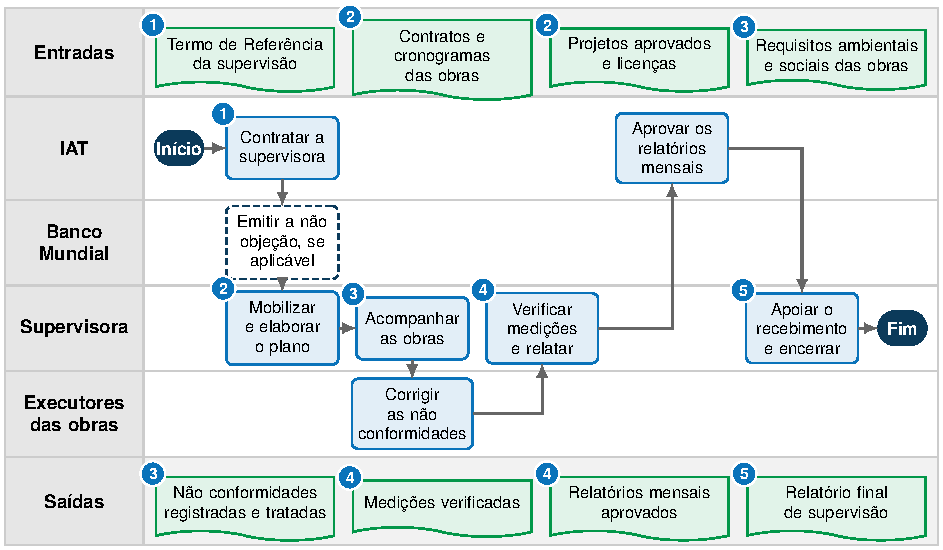
\includegraphics[width=15.96cm]{figuras/g-raias-3227.pdf}
  \fonteMOP{Fonte: IAT (2026).}
  % Texto alternativo: Fluxograma em raias da supervisão e gerenciamento das obras, com uma raia por instituição, as etapas numeradas na raia do executor, as entradas no topo e as saídas na base.
\end{figure}

\begin{figure}[H]
  \centering
  \caption{Ciclo mensal de supervisão das obras}\label{ciclo-supervisao}
  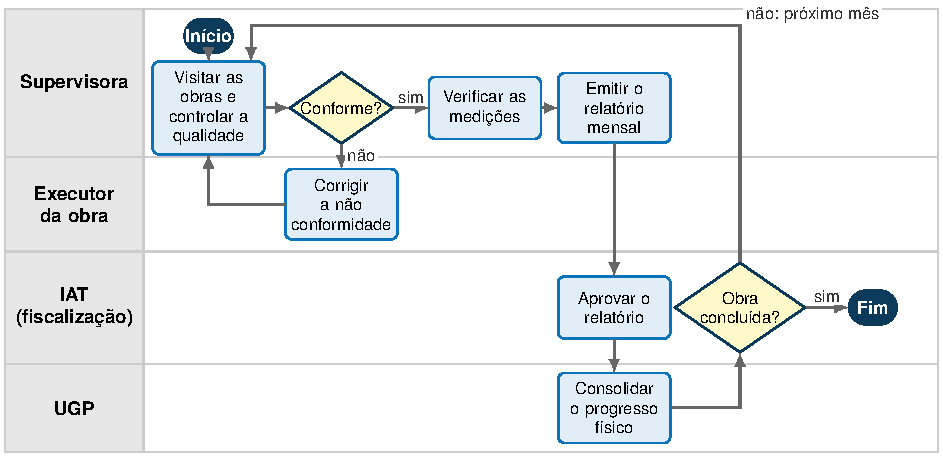
\includegraphics[width=15.96cm]{figuras/f-ciclo-supervisao.pdf}
  \fonteMOP{Fonte: IAT (2026).}
  % Texto alternativo: Fluxograma em raias do ciclo mensal de supervisão, com a correção das não conformidades, a aprovação do relatório pelo IAT, a consolidação pela UGP e a repetição mensal até a conclusão das obras.
\end{figure}

\phantomsection
\subsubsection*{4.1 Etapa 1: Contratação da supervisora}

\textbf{Atividades:} elaboração do Termo de Referência, com escopo, equipe e produtos; seleção da consultoria pelo método definido no Plano de Aquisições; assinatura do contrato e emissão da ordem de serviço.

\textbf{Entradas:} cronogramas previstos das obras; Termo de Referência.

\textbf{Responsáveis:} IAT (executa e aprova); UGP e Banco Mundial (consultados).

\textbf{Produto:} contrato assinado.

\phantomsection
\subsubsection*{4.2 Etapa 2: Mobilização e plano de supervisão}

\textbf{Atividades:} mobilização da equipe; elaboração do plano de supervisão, com procedimentos de medição, de controle de qualidade e de registro das não conformidades; implantação do sistema de registro e de relatórios.

\textbf{Entradas:} contrato; projetos aprovados; contratos das obras.

\textbf{Responsáveis:} supervisora (executa); IAT (aprova).

\textbf{Produto:} plano de supervisão aprovado.

\phantomsection
\subsubsection*{4.3 Etapa 3: Acompanhamento das obras}

\textbf{Atividades:} visitas de campo; controle de qualidade dos materiais e dos serviços; verificação dos requisitos ambientais, sociais e de saúde e segurança do trabalho; registro das não conformidades e acompanhamento da correção.

\textbf{Entradas:} plano de supervisão; obras em execução.

\textbf{Responsáveis:} supervisora (executa); executores das obras (corrigem); IAT (aprova).

\textbf{Produto:} registros de campo e de não conformidades.

\phantomsection
\subsubsection*{4.4 Etapa 4: Medições e relatórios}

\textbf{Atividades:} verificação das medições dos executores; controle de prazos e custos; relatórios mensais ao IAT, com as informações de progresso destinadas à UGP.

\textbf{Entradas:} registros de campo; medições dos executores.

\textbf{Responsáveis:} supervisora (executa); IAT (aprova); UGP (informada).

\textbf{Produto:} relatórios mensais aprovados.

\phantomsection
\subsubsection*{4.5 Etapa 5: Recebimento das obras e encerramento}

\textbf{Atividades:} apoio ao recebimento provisório e definitivo das obras; conferência dos projetos \textit{as built}; relatório final de supervisão.

\textbf{Entradas:} obras concluídas; relatórios mensais.

\textbf{Responsáveis:} supervisora (executa); IAT (aprova).

\textbf{Produto:} relatório final de supervisão.

\phantomsection
\subsubsection*{4.6 Modalidade de execução}

O item de custo é a supervisão e o gerenciamento de obras: 36 profissionais-mês a R\$~299.722,20, no total de R\$~10,79 milhões, com recursos do empréstimo do BIRD. A execução ocorre mediante licitação de serviços de consultoria, conforme o Caderno AQ.

\pendencia{A supervisão está prevista de 2029 a 2032, e as obras de abastecimento estendem-se de 2028 a 2033. Avaliar a supervisão das obras de 2028 e de 2033 e confirmar se o escopo inclui as instalações de esgotamento sanitário.}

\phantomsection
\addcontentsline{toc}{subsection}{5. Matriz de responsabilidades}
\subsection*{5. Matriz de responsabilidades}

O Quadro~\ref{raci-3227} apresenta o papel de cada parte em cada etapa.

\begin{quadro}[H]
  \caption{Matriz de responsabilidades da supervisão e gerenciamento das obras}\label{raci-3227}
  \footnotesize\renewcommand{\arraystretch}{1.25}\setlength{\tabcolsep}{3pt}
  \begin{tabular}{>{\raggedright\arraybackslash}p{\dimexpr 0.2536\linewidth-2\tabcolsep\relax}>{\centering\arraybackslash}p{\dimexpr 0.0882\linewidth-2\tabcolsep\relax}>{\centering\arraybackslash}p{\dimexpr 0.0882\linewidth-2\tabcolsep\relax}>{\centering\arraybackslash}p{\dimexpr 0.0882\linewidth-2\tabcolsep\relax}>{\centering\arraybackslash}p{\dimexpr 0.0882\linewidth-2\tabcolsep\relax}>{\centering\arraybackslash}p{\dimexpr 0.0882\linewidth-2\tabcolsep\relax}>{\centering\arraybackslash}p{\dimexpr 0.3055\linewidth-2\tabcolsep\relax}}
    \rowcolor{azulEscuro}\textcolor{white}{\textbf{Parte}} & \textcolor{white}{\textbf{E1}} & \textcolor{white}{\textbf{E2}} & \textcolor{white}{\textbf{E3}} & \textcolor{white}{\textbf{E4}} & \textcolor{white}{\textbf{E5}} & \textcolor{white}{\textbf{Produto final}} \\
    IAT & \raci{R} \raci{A} & \raci{A} & \raci{A} & \raci{A} & \raci{A} & \raci{A} \\ \arrayrulecolor{cinza20}\hline
    \rowcolor{cinza5}Supervisora & – & \raci{R} & \raci{R} & \raci{R} & \raci{R} & \raci{R} \\ \arrayrulecolor{cinza20}\hline
    Executores das obras & – & \raci{C} & \raci{R} & \raci{C} & \raci{C} & \raci{I} \\ \arrayrulecolor{cinza20}\hline
    \rowcolor{cinza5}Prefeituras & – & \raci{I} & \raci{I} & – & \raci{I} & \raci{I} \\ \arrayrulecolor{cinza20}\hline
    UGP & \raci{C} & \raci{I} & \raci{I} & \raci{I} & \raci{I} & \raci{I} \\ \arrayrulecolor{cinza20}\hline
    \rowcolor{cinza5}Banco Mundial & \raci{C} & – & – & – & – & – \\ \noalign{\global\arrayrulewidth=1pt}\arrayrulecolor{azulEscuro}\hline\noalign{\global\arrayrulewidth=0.4pt}
  \end{tabular}
  \fonteMOP{Fonte: IAT (2026).}
  \notaMOP{Nota: E1 a E5 correspondem às Etapas 1 a 5 do item 4. \raci{R} executa (pode haver mais de um); \raci{A} aprova ou valida o produto (um por etapa); \raci{C} é consultado previamente; \raci{I} é informado posteriormente. Produto final: obras supervisionadas, com relatórios aprovados.}
\end{quadro}

\phantomsection
\addcontentsline{toc}{subsection}{6. Metas, indicadores e comprovação}
\subsection*{6. Metas, indicadores e comprovação}

A meta física é expressa em profissionais-mês, de 2029 a 2032 (Quadro~\ref{metas-3227}).

\begin{quadro}[H]
  \caption{Metas anuais da supervisão e gerenciamento das obras}\label{metas-3227}
  \footnotesize\renewcommand{\arraystretch}{1.25}\setlength{\tabcolsep}{3pt}
  \begin{tabular}{>{\raggedright\arraybackslash}p{\dimexpr 0.2095\linewidth-2\tabcolsep\relax}>{\raggedright\arraybackslash}p{\dimexpr 0.1268\linewidth-2\tabcolsep\relax}>{\raggedleft\arraybackslash}p{\dimexpr 0.0794\linewidth-2\tabcolsep\relax}>{\raggedleft\arraybackslash}p{\dimexpr 0.0794\linewidth-2\tabcolsep\relax}>{\raggedleft\arraybackslash}p{\dimexpr 0.0794\linewidth-2\tabcolsep\relax}>{\raggedleft\arraybackslash}p{\dimexpr 0.0794\linewidth-2\tabcolsep\relax}>{\raggedleft\arraybackslash}p{\dimexpr 0.0794\linewidth-2\tabcolsep\relax}>{\raggedleft\arraybackslash}p{\dimexpr 0.0794\linewidth-2\tabcolsep\relax}>{\raggedleft\arraybackslash}p{\dimexpr 0.0794\linewidth-2\tabcolsep\relax}>{\raggedleft\arraybackslash}p{\dimexpr 0.1081\linewidth-2\tabcolsep\relax}}
    \rowcolor{azulEscuro}\textcolor{white}{\textbf{Produto}} & \textcolor{white}{\textbf{Unidade}} & \centering\arraybackslash \textcolor{white}{\textbf{Ano 1}} & \centering\arraybackslash \textcolor{white}{\textbf{Ano 2}} & \centering\arraybackslash \textcolor{white}{\textbf{Ano 3}} & \centering\arraybackslash \textcolor{white}{\textbf{Ano 4}} & \centering\arraybackslash \textcolor{white}{\textbf{Ano 5}} & \centering\arraybackslash \textcolor{white}{\textbf{Ano 6}} & \centering\arraybackslash \textcolor{white}{\textbf{Ano 7}} & \centering\arraybackslash \textcolor{white}{\textbf{Total}} \\
    Supervisão e gerenciamento de obras & prof.-mês & – & – & 6 & 12 & 12 & 6 & – & 36 \\ \noalign{\global\arrayrulewidth=1pt}\arrayrulecolor{azulEscuro}\hline\noalign{\global\arrayrulewidth=0.4pt}
  \end{tabular}
  \fonteMOP{Fonte: Planilha PSH\_CUSTO\_Consolidada, versão v2408 (PARANÁ, 2026).}
  \notaMOP{Nota: Ano 1 = 2027 e Ano 7 = 2033. Prof.-mês = profissionais-mês.}
\end{quadro}

Os indicadores constam do Quadro~\ref{ind-3227}, e os critérios de aceite, do Quadro~\ref{aceite-3227}.

\begin{quadro}[H]
  \caption{Indicadores da supervisão e gerenciamento das obras}\label{ind-3227}
  \footnotesize\renewcommand{\arraystretch}{1.25}\setlength{\tabcolsep}{3pt}
  \begin{tabular}{>{\raggedright\arraybackslash}p{\dimexpr 0.3165\linewidth-2\tabcolsep\relax}>{\raggedright\arraybackslash}p{\dimexpr 0.1378\linewidth-2\tabcolsep\relax}>{\raggedleft\arraybackslash}p{\dimexpr 0.1102\linewidth-2\tabcolsep\relax}>{\raggedleft\arraybackslash}p{\dimexpr 0.1599\linewidth-2\tabcolsep\relax}>{\raggedright\arraybackslash}p{\dimexpr 0.2756\linewidth-2\tabcolsep\relax}}
    \rowcolor{azulEscuro}\textcolor{white}{\textbf{Indicador}} & \textcolor{white}{\textbf{Unidade}} & \centering\arraybackslash \textcolor{white}{\textbf{Linha de base (2025)}} & \centering\arraybackslash \textcolor{white}{\textbf{Meta}} & \textcolor{white}{\textbf{Frequência e fonte dos dados}} \\
    Relatórios de supervisão aprovados & relatórios & 0 & 1 por mês de supervisão & Mensal; IAT \\ \arrayrulecolor{cinza20}\hline
    \rowcolor{cinza5}Sistemas de abastecimento supervisionados com Termo de Recebimento Definitivo & sistemas & 0 & 83 & Semestral; IAT \\ \arrayrulecolor{cinza20}\hline
    Não conformidades corrigidas no prazo & \% das registradas & – & 100 & Mensal; relatórios de supervisão \\ \noalign{\global\arrayrulewidth=1pt}\arrayrulecolor{azulEscuro}\hline\noalign{\global\arrayrulewidth=0.4pt}
  \end{tabular}
  \fonteMOP{Fonte: IAT (2026).}
\end{quadro}

\pendencia{Definir no Termo de Referência o número de relatórios e a distribuição dos 36 profissionais-mês entre as frentes de obra.}

\begin{quadro}[H]
  \caption{Critérios de aceite e evidências da supervisão e gerenciamento das obras}\label{aceite-3227}
  \footnotesize\renewcommand{\arraystretch}{1.25}\setlength{\tabcolsep}{5pt}
  \begin{tabular}{>{\raggedright\arraybackslash}p{\dimexpr 0.2150\linewidth-2\tabcolsep\relax}>{\raggedright\arraybackslash}p{\dimexpr 0.3386\linewidth-2\tabcolsep\relax}>{\raggedright\arraybackslash}p{\dimexpr 0.2921\linewidth-2\tabcolsep\relax}>{\raggedright\arraybackslash}p{\dimexpr 0.1543\linewidth-2\tabcolsep\relax}}
    \rowcolor{azulEscuro}\textcolor{white}{\textbf{Produto}} & \textcolor{white}{\textbf{Critério de aceite}} & \textcolor{white}{\textbf{Evidência de comprovação}} & \textcolor{white}{\textbf{Responsável pela validação}} \\
    Plano de supervisão & Procedimentos de medição, qualidade e registro definidos & Plano aprovado & IAT \\ \arrayrulecolor{cinza20}\hline
    \rowcolor{cinza5}Relatório mensal & Andamento, medições, não conformidades e conformidade ambiental e social de cada frente & Relatório aprovado & IAT \\ \arrayrulecolor{cinza20}\hline
    Medições verificadas & Quantidades conferidas em campo & Boletins de medição atestados & IAT \\ \arrayrulecolor{cinza20}\hline
    \rowcolor{cinza5}Relatório final & Consolida a supervisão e o recebimento das obras & Relatório final aprovado & IAT \\ \noalign{\global\arrayrulewidth=1pt}\arrayrulecolor{azulEscuro}\hline\noalign{\global\arrayrulewidth=0.4pt}
  \end{tabular}
  \fonteMOP{Fonte: IAT (2026).}
\end{quadro}

\phantomsection
\addcontentsline{toc}{subsection}{7. Gestão de riscos e impactos ambientais e sociais}
\subsection*{7. Gestão de riscos e impactos ambientais e sociais}

A supervisora constitui instrumento de cumprimento das NAS nas obras, mediante verificação em campo dos requisitos ambientais, sociais e de saúde e segurança aplicáveis às ações de abastecimento de água e de esgotamento sanitário (Quadro~\ref{nas-3227}). As demais NAS são tratadas nas respectivas ações.

\begin{quadro}[H]
  \caption{Aplicação das Normas Ambientais e Sociais à supervisão e gerenciamento das obras}\label{nas-3227}
  \footnotesize\renewcommand{\arraystretch}{1.25}\setlength{\tabcolsep}{5pt}
  \begin{tabular}{>{\raggedright\arraybackslash}p{\dimexpr 0.1874\linewidth-2\tabcolsep\relax}>{\raggedright\arraybackslash}p{\dimexpr 0.3716\linewidth-2\tabcolsep\relax}>{\raggedright\arraybackslash}p{\dimexpr 0.4410\linewidth-2\tabcolsep\relax}}
    \rowcolor{azulEscuro}\textcolor{white}{\textbf{NAS}} & \textcolor{white}{\textbf{Aplicação à ação}} & \textcolor{white}{\textbf{Medidas e instrumentos}} \\
    NAS 1 – Avaliação e gestão de riscos & Acompanhamento dos planos ambientais e sociais das obras & Verificação e registro em cada relatório mensal (MGAS) \\ \arrayrulecolor{cinza20}\hline
    \rowcolor{cinza5}NAS 2 – Condições de trabalho & Trabalhadores das obras e da própria supervisora & Verificação de EPI, treinamentos e registros de incidentes (Procedimentos de Gestão de Mão de Obra) \\ \arrayrulecolor{cinza20}\hline
    NAS 4 – Saúde e segurança da comunidade & Sinalização e isolamento das obras nas comunidades & Inspeção de campo e exigência de correção imediata \\ \arrayrulecolor{cinza20}\hline
    \rowcolor{cinza5}NAS 10 – Engajamento das partes interessadas & Queixas relacionadas às obras & Registro e encaminhamento ao Mecanismo de Queixas e Reclamações (MQR) \\ \noalign{\global\arrayrulewidth=1pt}\arrayrulecolor{azulEscuro}\hline\noalign{\global\arrayrulewidth=0.4pt}
  \end{tabular}
  \fonteMOP{Fonte: IAT (2026), com base nos instrumentos do Caderno AS.}
\end{quadro}

\phantomsection
\addcontentsline{toc}{subsection}{8. Cronograma}
\subsection*{8. Cronograma}

A contratação ocorre em 2028, a mobilização em 2029 e a supervisão de 2029 a 2032, com 6 profissionais-mês em 2029, 12 em 2030 e em 2031 e 6 em 2032 (Figura~\ref{crono-3227}).

\begin{figure}[H]
  \centering
  \caption{Cronograma das etapas e das entregas da supervisão e gerenciamento das obras}\label{crono-3227}
  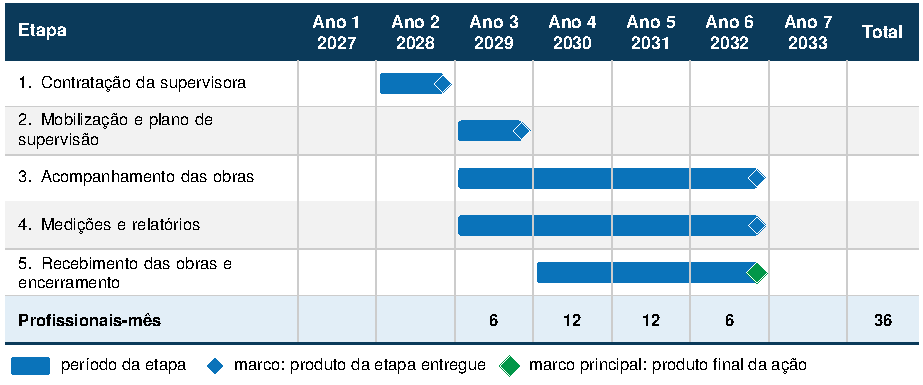
\includegraphics[width=15.64cm]{figuras/g-crono-3227.pdf}
  \fonteMOP{Fonte: IAT (2026), com quantidades da planilha PSH\_CUSTO\_Consolidada (PARANÁ, 2026).}
  % Texto alternativo: Cronograma anual de 2027 a 2033 com as etapas e as quantidades a entregar da supervisão e gerenciamento das obras.
\end{figure}

\phantomsection
\addcontentsline{toc}{subsection}{9. Interfaces e dependências}
\subsection*{9. Interfaces e dependências}

A ação depende dos contratos, dos projetos e dos cronogramas das obras de abastecimento de água e de esgotamento sanitário. Fornece ao IAT os relatórios que fundamentam as medições, os pagamentos e o recebimento das obras, aos executores as não conformidades a corrigir e à UGP as informações de progresso físico e de conformidade (Figura~\ref{interf-3227}).

\begin{figure}[H]
  \centering
  \caption{Interfaces e dependências da supervisão e gerenciamento das obras}\label{interf-3227}
  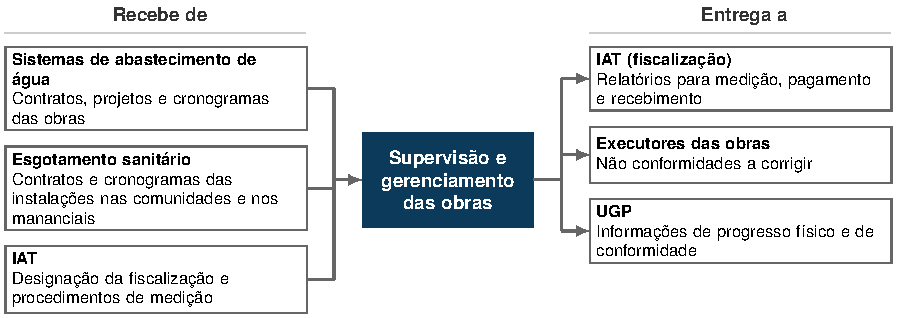
\includegraphics[width=15.30cm]{figuras/g-interf-3227.pdf}
  \fonteMOP{Fonte: IAT (2026).}
  % Texto alternativo: Diagrama das interfaces da supervisão e gerenciamento das obras: insumos recebidos de outras partes do Programa e produtos entregues a elas.
\end{figure}

\phantomsection
\addcontentsline{toc}{subsection}{10. Documentos complementares}
\subsection*{10. Documentos complementares}

\begin{itemize}
  \item Termo de Referência da supervisão e do gerenciamento das obras (a elaborar);
  \item Regulamento de Aquisições do Banco Mundial para mutuários de Financiamento de Projetos de Investimento e Caderno AQ;
  \item Caderno AS;
  \item Normas técnicas aplicáveis às obras (ABNT) e projetos aprovados de cada sistema.
\end{itemize}


% =====================================================================
%  ELEMENTOS PÓS-TEXTUAIS
% =====================================================================
\postextual
\chapter*{Referências}
\addcontentsline{toc}{chapter}{Referências}
\begin{SingleSpacing}\raggedright
\noindent ASSOCIAÇÃO BRASILEIRA DE NORMAS TÉCNICAS (ABNT). \textbf{NBR 12244}: poço tubular: construção de poço tubular para captação de água subterrânea. Rio de Janeiro: ABNT, 2006.\par\medskip
\noindent ASSOCIAÇÃO BRASILEIRA DE NORMAS TÉCNICAS (ABNT). \textbf{NBR 12212}: projeto de poço tubular para captação de água subterrânea: procedimento. Rio de Janeiro: ABNT, 2017.\par\medskip
\noindent ASSOCIAÇÃO BRASILEIRA DE NORMAS TÉCNICAS (ABNT). \textbf{NBR 17076}: projeto de sistema de tratamento de esgoto de menor porte: requisitos. Rio de Janeiro: ABNT, 2024.\par\medskip
\noindent BAHIA. Governo do Estado. \textbf{Centrais de abastecimento de associações são referência de política pública de saneamento rural}. Salvador, 2022. Disponível em: \url{https://www.ba.gov.br/comunicacao/2022/05/noticias/centrais-de-abastecimento-de-associacoes-sao-referencia-de-politica-publica-de-saneamento-rural}.\par\medskip
\noindent BANCO MUNDIAL. \textbf{Quadro Ambiental e Social}. Washington, DC: Banco Mundial, 2017.\par\medskip
\noindent BRASIL. \textbf{Lei nº~9.433, de 8 de janeiro de 1997}. Institui a Política Nacional de Recursos Hídricos, cria o Sistema Nacional de Gerenciamento de Recursos Hídricos, regulamenta o inciso XIX do art. 21 da Constituição Federal, e altera o art. 1º da Lei nº~8.001, de 13 de março de 1990, que modificou a Lei nº~7.990, de 28 de dezembro de 1989. Brasília, DF: Presidência da República, 1997.\par\medskip
\noindent BRASIL. \textbf{Lei nº~11.107, de 6 de abril de 2005}. Dispõe sobre normas gerais de contratação de consórcios públicos e dá outras providências. Brasília, DF: Presidência da República, 2005.\par\medskip
\noindent BRASIL. \textbf{Lei nº~11.445, de 5 de janeiro de 2007}. Estabelece as diretrizes nacionais para o saneamento básico [...]. Brasília, DF: Presidência da República, 2007.\par\medskip
\noindent BRASIL. \textbf{Lei nº~13.019, de 31 de julho de 2014}. Estabelece o regime jurídico das parcerias entre a administração pública e as organizações da sociedade civil. Brasília, DF: Presidência da República, 2014.\par\medskip
\noindent BRASIL. \textbf{Lei nº~13.709, de 14 de agosto de 2018}. Lei Geral de Proteção de Dados Pessoais (LGPD). Brasília, DF: Presidência da República, 2018.\par\medskip
\noindent BRASIL. Ministério da Saúde. Fundação Nacional de Saúde. \textbf{Programa Nacional de Saneamento Rural}. Brasília, DF: Funasa, 2019.\par\medskip
\noindent BRASIL. \textbf{Lei nº~14.026, de 15 de julho de 2020}. Atualiza o marco legal do saneamento básico e altera a Lei nº~9.984, de 17 de julho de 2000, [...]. Brasília, DF: Presidência da República, 2020.\par\medskip
\noindent BRASIL. Ministério da Saúde. \textbf{Portaria GM/MS nº~888, de 4 de maio de 2021}. Altera o Anexo XX da Portaria de Consolidação GM/MS nº~5, de 28 de setembro de 2017, para dispor sobre os procedimentos de controle e de vigilância da qualidade da água para consumo humano e seu padrão de potabilidade. Brasília, DF: Ministério da Saúde, 2021.\par\medskip
\noindent BRASIL. \textbf{Decreto nº~11.599, de 12 de julho de 2023}. Dispõe sobre a prestação regionalizada dos serviços públicos de saneamento básico, o apoio técnico e financeiro de que trata o art. 13 da Lei nº~14.026, de 15 de julho de 2020, a alocação de recursos públicos federais e os financiamentos com recursos da União ou com recursos geridos ou operados por órgãos ou entidades da União de que trata o art. 50 da Lei nº~11.445, de 5 de janeiro de 2007. Brasília, DF: Presidência da República, 2023.\par\medskip
\noindent BRASIL. Ministério da Saúde. Fundação Nacional de Saúde. \textbf{Portaria nº~2.777, de 30 de julho de 2025}. Brasília, DF: Funasa, 2025. Disponível em: \url{https://bvs.saude.gov.br/bvs/saudelegis/funasa/2025/prt2777_05_08_2025.html}.\par\medskip
\noindent CEARÁ. Governo do Estado. \textbf{Modelo cearense de saneamento rural sustentável alcança mais de 1,1 milhão de pessoas no campo}. Fortaleza, 16 out. 2025. Disponível em: \url{https://www.ceara.gov.br/2025/10/16/modelo-cearense-de-saneamento-rural-sustentavel-alcanca-mais-de-11-milhao-de-pessoas-no-campo/}.\par\medskip
\noindent INSTITUTO ÁGUA E TERRA (IAT). \textbf{Nota técnica}: Componente 3 – Segurança Hídrica para o Saneamento; Subcomponente 3.2 – Saneamento Rural. Curitiba: IAT, 2026a. Documento interno, versão de 4 mar. 2026.\par\medskip
\noindent INSTITUTO ÁGUA E TERRA (IAT). \textbf{Nota técnica}: Subcomponente 3.2.b – implantação e reabilitação de sistemas coletivos de abastecimento de água e esgotamento sanitário no meio rural. Curitiba: IAT, 2026b. Documento interno.\par\medskip
\noindent INSTITUTO ÁGUA E TERRA (IAT); INSTITUTO DE DESENVOLVIMENTO RURAL DO PARANÁ (IDR-PARANÁ). \textbf{Saneamento rural}: áreas prioritárias, associações de municípios, CISPAR e concentração de domicílios rurais. Curitiba, 2025. 1 mapa, formato A3.\par\medskip
\noindent INSTITUTO BRASILEIRO DE GEOGRAFIA E ESTATÍSTICA (IBGE). \textbf{Censo Demográfico 2022}: agregados por setores censitários. Rio de Janeiro: IBGE, 2024.\par\medskip
\noindent PARANÁ. \textbf{Lei nº~12.726, de 26 de novembro de 1999}. Institui a Política Estadual de Recursos Hídricos e adota outras providências. Curitiba: Assembleia Legislativa do Estado do Paraná, 1999.\par\medskip
\noindent PARANÁ. Secretaria de Estado do Planejamento. \textbf{Planilha de custos do PSH-PR}: PSH\_CUSTO\_Consolidada, versão v2408. Curitiba: SEPL, 2026. Documento interno.\par\medskip
\noindent SANEPAR – COMPANHIA DE SANEAMENTO DO PARANÁ. \textbf{Manual do Programa Sanepar Rural}. Curitiba: Sanepar, [s.d.]. Documento interno.\par\medskip
\noindent TONETTI, Adriano Luiz \textit{et al.} \textbf{Tratamento de esgotos domésticos em comunidades isoladas}: referencial para a escolha de soluções. Campinas: Unicamp, 2018.\par\medskip
\end{SingleSpacing}

\chapter*{Glossário complementar}
\addcontentsline{toc}{chapter}{Glossário complementar}
Os termos abaixo complementam o glossário geral do MOP.

\noindent\textbf{Contratação integrada:} regime de execução em que a mesma empresa elabora os projetos e executa as obras de cada sistema.\par\smallskip
\noindent\textbf{Entidade gestora:} associação, central de associações ou consórcio público responsável pela operação e pela manutenção do sistema após a entrega.\par\smallskip
\noindent\textbf{Modelo de gestão:} arranjo institucional, jurídico e financeiro que define a entidade responsável pela operação, pela manutenção e pela cobrança dos serviços de saneamento rural.\par\smallskip
\noindent\textbf{Plano Integrado de Propriedade (PIP):} plano elaborado pelo serviço de assistência técnica e extensão rural contratado no Componente 2 para cada propriedade rural aderente ao PSH-PR, com as práticas e as intervenções recomendadas.\par\smallskip
\noindent\textbf{Sistema coletivo de abastecimento de água:} conjunto de captação, tratamento, reservação, rede de distribuição e ligações domiciliares que abastece uma comunidade.\par\smallskip
\noindent\textbf{Solução individual de esgotamento sanitário:} sistema descentralizado que coleta, trata e promove a disposição final do esgoto de um domicílio no próprio lote.\par\smallskip
\noindent\textbf{Termo de Recebimento Definitivo (TRD):} documento que formaliza o recebimento final do sistema pelo IAT, após a pré-operação e o aceite da entidade gestora.\par\smallskip
\noindent\textbf{Trabalho técnico-social:} conjunto de atividades de mobilização, cadastro, diagnóstico, educação sanitária e ambiental e organização comunitária junto às famílias.\par\smallskip
\noindent\textbf{Unidade regional de apoio:} estrutura do modelo de gestão, com equipe técnica, sede e veículo, que presta suporte técnico às associações de uma região.\par\smallskip


\ifmostrarpendencias
  \chapter*{Lista de pendências}
  \addcontentsline{toc}{chapter}{Lista de pendências}
  \makeatletter\@starttoc{tdo}\makeatother
\fi

\end{document}
